\documentclass[11pt]{article}		% Sets font size and document type
\usepackage{fontspec}				% Allows us to use custom fonts
\usepackage{graphicx}				% Does pictures
\usepackage{parskip}				% Removes paragraph indents and adds a vertical space
\usepackage{multicol}				% Allows for multiple columns
\usepackage{titlesec}				% Changes section title appearance
\usepackage{setspace}				% Allows you to set line spacing
\usepackage{amsmath}				% Maths typesetting
\usepackage[margin=20 mm]{geometry}	% Sets page margin
\PassOptionsToPackage{hyphens}{url}\usepackage[colorlinks=true,linkcolor=blue,citecolor=blue,urlcolor=blue]{hyperref}	
									% Allows for hypertext for references (links) - edited to hake links look like normal text rather than having a border
\doublespacing						% Double spaces - this annoys me but is unavoidable I think
\usepackage{float} %allows an image to be placed exactly where you want it

%Add any more packages needed here:
\usepackage[justification=centering,font=small]{caption}	
									% Centres captions and makes them smaller
\usepackage[none]{hyphenat}			% Lines end cleanly - no hyphenation mid word
\usepackage{fancyhdr}				% Nicer headers/footers
\usepackage{amssymb}				% Allows for more maths symbols including not less than
\usepackage{wrapfig}				% Wrap figures
\usepackage{longtable}				% Allows for long multi page tables - mainly for pains and gains section
\usepackage{array}
\usepackage[table]{xcolor}			% Allows the latex table to be coloured to match other formatting
\usepackage{floatflt}               % Another package for doing wrapped figures
\usepackage{ragged2e}               % Makes the mega table look nicer

% Makes it so all equations have full sized numbers, independent of font size used		
\makeatletter
\def\tagform@#1{\maketag@@@{\normalsize(#1)\@@italiccorr}}
\makeatother

% There is some scope for changing the paragraph spacing and spacing around section headers if you are short of space

\graphicspath{{Images/}}	% Images are in a folder called 'Images'

% Set a variable for image height, so all images are the same size and easy to change
\newlength{\imageheight}	 % Creates the variable
\setlength{\imageheight}{0.25\textwidth}  % Sets the variable

\newcommand{\supercite}[1]{\textsuperscript{\cite{#1}}}		% New command to cite things in superscript without having to type it out every time

\newcommand{\figref}[1]{\hyperref[#1]{Figure \ref*{#1}}}    % New command to automatically fill out basic figure references more easily

\newcommand{\equationref}[1]{\hyperref[#1]{Equation \ref*{#1}}}     % New command to automatically fill out equation references more easily

\newcommand{\tableref}[1]{\hyperref[#1]{Table \ref*{#1}}}     % New command to automatically fill out table references more easily

\newcommand{\sectref}[1]{\hyperref[#1]{Section \ref*{#1}}}     % New command to automatically fill out section references more easily

\setcounter{tocdepth}{2}	% Means table of contents only shows subsections

% Use Arial
\setmainfont[
BoldFont=Arial Bold.ttf,
ItalicFont=Arial Italic.ttf,
BoldItalicFont=Arial Bold Italic.ttf
]{Arial.ttf}

\def\columnseprulecolor{\color{black}} % Makes the separation line black

% Have got this working with TexStudio now - need to change compiler from default to XeLaTeX (Options > Configure TexStudio > Build > Default Compiler > XeLaTeX)
% Will be slow at first, but once the fonts have installed should work more quickly

% Overleaf link - https://www.overleaf.com/project/5fce665153f1701e8414d47b
\begin{document}
	
	\flushleft
	\raggedright

	\begin{center}
	
		\vspace*{1cm}
		
		\begin{figure}
			\centering
			\includegraphics[width=\textwidth]{PipeDreamLogo}
		\end{figure}
						
		\vspace*{-2cm}
		
		\fontsize{20pt}{22pt}\selectfont
		B3 THIRD YEAR PROJECT
		
		TEAM PipeDream
		
		\vspace*{1cm}
		
		\fontsize{12pt}{14pt}\selectfont		
		ENGINEERING, ENTREPRENEURSHIP AND MANAGEMENT PATHWAY
		
		\vspace*{0.5cm}
		
		\rule{0.95\textwidth}{1pt}

		\fontsize{20pt}{22pt}\selectfont
		Designing an Autonomous In-Pipe Inspection Robot
		
		\fontsize{12pt}{14pt}\selectfont
		Designing an Autonomous Service Robot
		
		%\vspace*{-1cm}
		
		\rule{0.95\textwidth}{1pt}
		
		\vspace*{1.5cm}
				
		\fontsize{12pt}{14pt}\selectfont
		Submitted by:
		
		\fontsize{14pt}{16pt}\selectfont
		MONTGOMERY BERESFORD
		
		LOUIS EMANUEL
		
		JOSHUA GEI
		
		JIM LANEY
		
		\fontsize{11pt}{\baselineskip}\selectfont
		\thispagestyle{empty} % Remove page number
	\end{center}

	\newpage
	
	\pagestyle{empty}
	
	\setlength{\headheight}{18pt}
	\fancyhead[l]{\includegraphics[height=\baselineskip]{PipeDreamLogoSmall.png}}
	
	\setlength{\columnsep}{1.5cm} % Increases column separation for the TOC
	\setlength{\columnseprule}{0.5pt} % Sets thickness of the separation line
	
	\begin{multicols*}{2}
		\RaggedRight
	    \tableofcontents
    \end{multicols*}
	
	\setlength{\columnsep}{10pt} % Sets column separation for rest of the document
	\setlength{\columnseprule}{0pt} % Removes the separation line for figures
	
	\newpage
    \pagestyle{fancy}
	\setcounter{page}{1}
	
	%\renewcommand{\headrulewidth}{0pt}

	\section[Introduction]{Introduction - Joshua Gei}
	
		Underground gas distribution pipelines span over 2 million kilometres across global infrastructure, comprising over 60\% of all underground pipelines\supercite{sönnichsen_5_2021}, and are essential in the transport of natural gas for a variety of purposes, such as power generation for industrial and residential usage\supercite{group.met.com}. 
		\\
		\hspace*{2ex}However, gas pipeline failures due to leaks are commonplace, largely due to wear-and-tear and corrosion around pipe joints\supercite{corrosion1}. Unchecked leakages lead to transport delays, environmental damage, and potentially hazardous incidents\supercite{hazardousincidents}. Hence, adequate inspection and maintenance of gas pipelines are key priorities for gas distribution companies (GDCs), which cumulatively spent over £11.2 billion on inspection, maintenance  and replacement of gas pipelines globally in 2019\supercite{ltd}. 
		\\
		\hspace*{2ex}Currently, almost all inspection and maintenance of buried gas pipelines is performed manually\supercite{manually}, where roads are first excavated, and operators then manually inspect and fix leakages. This is illustrated below in \hyperref[excavation]{Figures \ref*{excavation} \& \ref*{pipelineRepair}}.
		\begin{figure}[h]
					\centering
					\begin{multicols}{2}
						\includegraphics[height=\imageheight]{Pipeline Excavation.jpg}
						\caption{Extensive excavation of entire pipeline\supercite{excavationpipeline}}
						\label{excavation}
						\columnbreak
						\includegraphics[height=\imageheight]{Pipeline Repair.jpg}
						\caption{Operators on-site performing manual inspection and maintenance\supercite{manualinspection}}
						\label{pipelineRepair}
					\end{multicols}
				\end{figure}
		\vspace{-0.75cm}
		\\The heavy amount of excavation required and the relatively slow and costly process of manual inspection poses pressing pain-points for GDCs, as well as other stakeholders such as local councils and the general public. Hence, PipeDream will seek to address these pain points with AccoBot, an \textbf{A}utonomous \textbf{C}rack, \textbf{C}orrosion and \textbf{O}bject Detection Ro\textbf{bot}.
		
	\subsection[Target Problems]{Target Problems - Joshua Gei}
	
	PipeDream will target specifically \textbf{Tier 3 underground gas distribution pipelines} in the UK, as they have the largest proportion of buried mains reaching or beyond their expected asset life, and require the most frequent maintenance and replacement\supercite{tier3}.
	
	\tableref{GasTiers} shows the pipeline assets categories used by all GDCs and regulators in the UK .
		\begin{table}[h]
			\centering
			\includegraphics[width=0.9\textwidth]{GasTiers}
			\caption{Pipeline assets category definitions\supercite{tier3}}
			\label{GasTiers}
 		\end{table}
 	
    \textbf{Problem 1: Manual Pipe Maintenance is Disruptive and Costly}
    \\Tier 3 mains are usually found in city locations, as opposed to other types of pipelines\supercite{tier3hse}. As such, multiple large excavations on busy roads are required to complete repairs. This causes extensive disruption to road users and results in high direct and indirect costs to GDCs, summarised below:
    		\begin{table}[h]
			\centering
			\includegraphics[width=0.9\textwidth]{costs.jpg}
			\caption{Direct and indirect costs of manual pipe inspection and maintenance}
			\label{PipeInspectionCosts}
 		\end{table}
 	\vspace{-0.5cm}
 	\\
    \hspace*{2ex}On average, a typical repair or replacement job takes around 3-10 days to complete, and cumulatively results in around 10,000 hours of traffic delays to all road users\supercite{pipeinspection}. Considering the cost of traffic delays alone, and using data from traffic analyst Inrix, which states that the average UK commuter loses 115 hours and £894 every year from road congestions\supercite{trafficreport}, the immediate costs faced by road users amounts to over £70,000 for a typical job. Road users pass on this pain to stakeholders such as local town councils and gas suppliers, which would in turn affect the prices of road permits and the amount gas suppliers are willing and able to pay GDCs. (More information on how different players in the gas industry interface with each other is shown in the Industry Value Chain in \sectref{valueChainSection})
 	
    \textbf{Problem 2: Significant Amounts of Functional Pipelines are Currently Being Decommissioned}
    \\
    Currently, around 9\% of all gas pipelines are being decommissioned each year\supercite{decommission}, and GDCs have indicated that the majority of these are Tier 3 pipelines\supercite{decommission}. However, it is usually unknown whether the pipes being decommissioned are actually damaged, due to the two reasons below:
	
	\textbf{Problem 2.1: Current Inspection Methods are Unable to Inspect all Types of Pipes }
	\\
	Most pipe-interior inspection methods currently rely on Pipeline Inspection Gauges or ‘PIGs’, alongside manual inspection which is limited to the exterior. PIGs are passive devices that are manually placed into the pipe and driven by the flow of fluid transport\supercite{pigging}, shown below in \hyperref[pig1]{Figures \ref*{pig1} \& \ref*{pig2}}.
		\begin{figure}[h]
					\centering
					\begin{multicols}{2}
						\includegraphics[height=0.22\textwidth]{pig1.jpg}
						\caption{PIG being inserted into underground pipeline\supercite{pigimage1}}
						\label{pig1}
						\columnbreak
						\includegraphics[width=0.45\textwidth]{pig2.jpg}
						\caption{PIG operation for water pipes - similar process for gas pipes\supercite{pigimage2}}
						\label{pig2}
					\end{multicols}
				\end{figure}
			\vspace{-0.75cm}
    \\
    \hspace*{2ex}However, PIGs are uncontrollable by external operators, and are unable to adapt to changes in pipe diameter, bends in the pipe, as well as vertical sections\supercite{piglimitations}. An estimated 20\% to 50\% by length of existing gas pipelines are ‘unpiggable’\supercite{unpiggable}, and cannot be inspected through manual inspection and PIGs. As such, the condition of the interior walls is unknown, and it is very difficult to determine replacement priority of the pipelines, resulting in pipelines simply being decommissioned and replaced at the end of their asset lives\supercite{decommission}.
    
    \textbf{Problem 2.2: Cost-benefit Analysis Results in Uninspected Pipelines Being Replaced}
    \\
    Additionally, GDCs usually perform a cost-benefit analysis to determine if pipelines are to be inspected and repaired or to be decommissioned and replaced\supercite{CBA}. Whenever the costs of inspection and maintenance outweighs the cost of replacement, GDCs opt for simply replacing pipelines, again resulting in replacement of possibly functional pipelines. 
    \\
    \hspace*{2ex}In total, it has been estimated that that through the use of advanced inspection techniques, savings from unnecessary pipeline replacement could be \textbf{up to £14,000 per km} a year\supercite{GRAID}. A correspondent from Wales and West Utilities has also informed PipeDream that they expect to save £0.5 million a year from a solution that reduces costs of Tier 3 pipes inspection\supercite{WWU}. 

	\subsection[Solution]{Solution - Joshua Gei}
	
    To the target problems faced by GDCs, PipeDream presents the \textbf{AccoBot} – an \textbf{A}utonomous \textbf{C}rack, \textbf{C}orrosion and \textbf{O}bject Detection Ro\textbf{Bot}. \\
    \hspace*{2ex}The AccoBot is an in-pipe robot that is able to autonomously navigate almost all types of pipes (including most ‘unpiggable’ pipes), pinpoint exact locations of pipe defects – namely areas where cracks and extensive corrosion are located – and generate a 3D map that operators are able to use to make minimal excavations to fix pipeline defects. 
%	\subsubsection[Value Proposition]{Value Proposition}
%	The main value propositions of AccoBot are as follows:
%        \begin{table}[h]
%			\centering
%			\includegraphics[width=0.9\textwidth]{ValueProposition.jpg}
%			\caption{Value Propositions of AccoBot to Gas Distribution Network Companies}
%			\label{VP}
% 		\end{table}
% 	\vspace{-0.2cm}
%	\\A detailed evaluation of our value proposition is performed in \sectref{solutionEvaluation} after further market analysis.

	\subsubsection[Product Description]{Product Description - Jim Laney}
	        
			AccoBot operates in Tier 3 pipes, with diameter from 457.2 mm to 914.4 mm, at any angle, and provides a map of the pipeline with failure locations for the gas distribution network.
			It reduces the disruption caused by having to excavate large areas of pipeline for inspection, since the issue can be located for a smaller, less disruptive excavation to take place.
			It provides an inspection method for pipes which cannot be inspected by PIGs, which only work in horizontal or near horizontal straight pipes\supercite{mills2017advances}.
			It enters a pipe using a launch tube, and travels autonomously along the inside of the pipe, checking for evidence of cracks and corrosion and logging their location for future maintenance.
			\begin{floatingfigure}[r]{0.45\textwidth}
			    \centering
				\includegraphics[width = 0.42\textwidth]{overviewCADLabels}
				\caption{3D CAD model of AccoBot with major components labelled}
				\label{3DSketch}
			\end{floatingfigure}
			\hspace*{2ex} While inside the pipe, AccoBot uses three legs to maintain contact with the pipe wall.
			Two legs can be rotated around the body of AccoBot to provide improved speed in different angled pipes, and all three legs can be extended and retracted to fit the current pipe diameter.
			It can navigate bends and pipes at different angles, without requiring prior knowledge, and will automatically feedback collected data to create an accurate map.
	%		\begin{figure}[h]
	%			\centering
	%			\includegraphics[trim={6cm 2cm 7cm 4cm}, clip, height = \imageheight]{overviewCAD}
	%			\caption{3D CAD model of AccoBot}
	%			\label{3DSketch}
	%		\end{figure}
			\begin{floatingfigure}[r]{0pt} \end{floatingfigure}
			\hspace*{2ex} AccoBot uses computer vision to identify cracks, corrosion and objects, and mark their location for maintenance.
			It then combines this with knowledge of its location to create a map of the pipe it has travelled and where different features occur, including bends.
			It uses object detection to identify important landmarks, such as connecting pipes, and possible pipe blockages, combing this with other pieces of data to determine its location along the pipeline.
			\\
			\hspace*{2ex} Its external location is transmitted using a small ELF transmitter, which communicates with GPS enabled external base stations. 
			Most communication between the robot and the operator is along a fibre optic cable connected to the robot, allowing for processing to take place off the robot.
			This cable transmits data quickly, and can also be used to retrieve the robot in the case of a failure.
			
			\subsubsection[Product User Journey]{Product User Journey - Joshua Gei} \label{userJourney}
			
            An illustration of how AccoBot works in practice is shown in \figref{userjourney}:
	        \begin{figure}[h]
				\centering
				\includegraphics[width=0.8\textwidth]{userjourneyfull.jpg}
				\caption{Product User Journey of AccoBot}
				\label{userjourney}
			\end{figure}

    \section{Market Research - EEM}
    
     Once a potential problem was identified, market research was carried out in order to specify the problem, and validate the existence and size of a market for a potential solution. 
        \\
        \hspace*{2ex}Firstly, it was determined that PipeDream would begin operating in the UK market, due to familiarity with legislation, availability of connections and funding, and being in closest proximity to PipeDream's base of operations in Oxford. 
        \\
        \hspace*{2ex}It was identified that GDCs in the UK will be PipeDream's key customers. In the UK, there are four key GDCs - SGN, Northen Gas Networks (NGN), Cadent Gas, and Wales and West Utilities (WWU), each operating as the sole gas distributor in their respective areas of operation, shown in \figref{distrit0}. 

        \subsection[Primary Market Research]{Primary Market Research - Montgomery Beresford} \label{primaryresearch}
            \begin{floatingfigure}[r]{0.4\textwidth}
    		    \centering
    	    	\includegraphics[width=0.32\textwidth]{distribution}
    		    \caption{GDC areas of operation\supercite{Gas_Distribution_Industry}}
        	    \label{distrit0}
    	    \end{floatingfigure}
   There is little detailed freely available information about the UK gas distribution industry, therefore once PipeDream identified GDCs as the likely clients, it was important to speak to people in their industry. Therefore PipeDream spoke to both innovation manages who are in charge of making the decisions about working with PipeDream, which is discussed in \sectref{go-to}, and to those those who worked closely with gas pipes in order to understand their pains, jobs and potential gains.
             The findings of this primary market research were used as a basis for the further research and analysis that is presented throughout the report, and were confirmed by research into sources such as GDC business plans and spending projections\supercite{SGN-GD2}, and third-party analysis of the industry\supercite{Gas_Distribution_Industry}. Moreover, the primary sources did not contradict each other and consistently reinforced what was heard from others, highlighting that this evidence is credible.
	        \begin{floatingfigure}[r]{0pt} \end{floatingfigure}
            \hspace*{2ex}In the first group PipeDream spoke to Thomas Barrett\supercite{Barret} a Network Engineer at Cadent and to David Ransome\supercite{Ransome}, an Engineering Services Manager at Cadent. In the second group Luccy Mason, Innovation Manager at Wales \& West Utilities, Michael Charlton, Innovation Implementation Manager at Northern Gas Networks, Gordon McMillan\supercite{McMillan}, Innovation Project Officer at SGN and Andrew Newton\supercite{Newton} who was Innovation Portfolio Manager at Cadent until June 2020 were spoken to.
	        \\
            \hspace*{2ex}Andrew Newton highlighted that the robot should be able to navigate bends and that most small size pipes have already been replaced and that the bigger mains in cities are more costly and difficult to repair. Therefore it was decided to further investigate these types of pipes. Additionally, he said that the capital outlay to buy a robot would be “prohibitive”\supercite{Newton}, which informed PipeDream's strategy, revenue model and pricing discussed in \sectref{businessmodel} .%\sectref{strategy} and \sectref{businessmodel}.
	        \\
            \hspace*{2ex}Thomas Barrett said that being able to inspect a live gas pipe without isolating it would make the robot “invaluable”\supercite{Barret}, which informed AccoBot's design. Andrew Newton further highlighted that, because the atmosphere is almost 100\% CH\textsubscript{4}, the robot’s interaction with the live gas conditions is not a big risk, but that the most dangerous part is the insertion of the robot, so it was decided to work with an experienced supplier to provide the launch tube system.
	        \\
            \hspace*{2ex}Additionally, competitors ULC and Synthotech, whom are analysed in \sectref{competitorAnalysis}, were spoken to gain an understanding of how existing robotic solutions fit into the industry. ULC suggested that larger gas distribution pipes of diameters 16-36 inches in urban areas would likely be the best part of the market to find a niche, confirming the findings from the interviews with employees at the GDCs. The contact said that to provide value the robot should be able to travel in both directions, map the pipe and assess the conditions\supercite{ULC_interview}. He also confirmed that using visual sensing combined with machine learning would be a viable and valuable inspection method, which Synthotech corroborated. %Discussions with Synthotech resulted in them offering to provide video and images to train the machine vision algorithms.
	        \\  \hspace*{2ex}
           Through this research PipeDream identified the market segment in which it would provide most value and have the greatest competitive advantage. This segment was Tier 3 iron distribution pipes that were either inaccessible to competitor robots or were too costly for other robots to fix.
%	 AccoBot has several applications which means that it will be operating in several small niches of the market. However for the revenue model PipeDream has assumed that initially only one of these applications are used. This is the function of inspecting joints to locate exactly which joints need to be replaced in a stretch of pipeline that would have all been replaced. 

%	Currently it is estimated that 30.8km of pipeline need to be replaced each year for the next 5 years. This has been calculated using the fact that SGN plans to replace 6.15km\supercite{SGN_Southern}\supercite{SGN_Scotland} and that NGN plans to replace 10.2km per year\supercite{NGN_decisions}. It was then assumed that the other two GDCs would have the same proportion of their pipelines as SGN that need replacing. Since joint failures are the most common failure it is likely that a large majority of these could be fixed by replacing the joints. In Tier 3 pipes there are roughly 0.275 joints per metre of pipeline\supercite{SGN_Southern} therefore it is estimated that there are 8474 joints that will be being removed by replacing the pipeline. Applying the £414.40 price per joint to these joints would give a market size of £3.5m. This form of revenue will be used for the revenue projections.

%	In addition to this SGN spent £7.2m on robotic intervention in 2020.\supercite{SGN_Scotland}\supercite{SGN_Southern} Assuming each company has a similar potential robotic intervention spend proportional to their total pipeline length then the total market spend on this a year would be £29m. Therefore the total potential market in the UK would be £37.19m. There is a difference in this compared to the top-down estimate of £57.6m being the size of the London market because the top-down estimate includes all types of pipes and not just the Tier 3 pipes. 
    		        
     %\subsubsection[Projected Market Penetration]{Projected Market Penetration - Montgomery Beresford}
    
    \subsection{Competitor Analysis} \label{competitorAnalysis}
        %There is clearly both a large market potential, and large potential for economic profit in this market. 
        Having understood the primary pains of the customer and identified a market segment to target, a competitor analysis was performed to understand the incumbent firms in the market.
        Since this is a relatively new industry which is at the beginning of a technology s-curve, there are a few competitors with very different designs, highlighting how no dominant design has emerged yet. The industry dynamics will be discussed in more detail in \sectref{industryP5F}. There are two major first-mover competitors in the UK in-pipe inspection industry who have clearly also identified the large potential for abnormal economic profit; these are Synthotech, which is part of Project GRAID, and ULC Robotics (ULC). ULC has much larger traction working with gas distribution companies but Synthotech has worked previously with SGN on the technology for Project GRAID, which focuses on the gas transmission networks, poses a potential future threat. In this section SWOT analysis is carried out for the two companies and ULC's products' features are compared to AccoBot's. The findings of this analysis helped inform PipeDream about their strategy to develop competitive advantages over these two firms and to capture a share of the market identified in \sectref{marketSizing}.

		\subsubsection[Project GRAID]{Project GRAID - Louis Emanuel}
		
			One potential competitor operating in the in-pipe inspection industry is project Gas Robot Agile Inspection Device (GRAID). Project GRAID is a joint project by the National Grid and three small and medium-sized enterprises. The project, which began in 2014, was given a budget of £5.6m to design and build a robot able to travel 100 metres around two bends taking visual readings\supercite{graidy}. As with AccoBot, it is targeting the live gas pipe market and aims to be able to navigate complex geometries. It is also able to operate in pipes with diameters between 762mm and 914.4mm. Therefore, it is necessary to perform the following SWOT analysis on the company.
			
			\textbf{Strengths} \\
			Project GRAID's key strength is its ongoing partnership with the National Grid. Although the National grid sold off its distribution network to the four leading GDCs\supercite{sellnetwork}, its history in the industry and extensive knowledge is an undeniable advantage for project GRAID. Furthermore, project GRAID has previously received funding from OFGEM's Network Innovation Competition. The competition is an annual opportunity for gas network companies to compete for funding for the development and demonstration of new technologies. This financial backing which amounted to a total of £5.6m reduces the need for high interest loans which are a significant fixed cost and barrier for new entrants as discussed in \sectref{industryP5F}. \\
		    \hspace*{2ex}Another significant strength of the GRAID project robot is its strong technical performance. Whilst CISBOT can operate at 99 psi, GRAID is capable of operating up to pressures of 1450 psi. Although the distribution pipeline usually operates at pressures below 200 psi, higher pressure pipes such as transmission lines can be pressured up to 1232 psi\supercite{transmissionpressure} meaning project GRAID could be a one stop shop for a range of pipes. Also, the need to inspect higher pressure pipes will make GRAID more competitive as the use of hydrogen gas becomes more common, because it requires higher distribution pressures due to its lower energy density, as described in \sectref{customerFuture}. 
	        
	        \textbf{Weaknesses}\\
	        Despite GRAID’s success, it does have weaknesses that could inhibit the success of the project moving forward. Firstly, whilst the National Grid operates the National Transmission system (NTS) which supplies gas to distribution companies like Cadent, it does not own any distribution networks. This is a significant disadvantage as the NTS is less than 1\% of the size of Cadents distribution network\supercite{NTSlength} and is easily inspected using PIG’s. This presents a challenge as ultimately, the robot must be sold or leased to these gas distribution networks in order to generate revenue. \\
	        \hspace*{2ex}Another weakness lies in the fact that along with the National grid, three other SMEs are also part of the GRAID project. Although it could be argued that this brings more knowledge to the project, the heavily regulated gas distribution industry is slow enough, and so having multiple significant shareholders could slow down decision making significantly. This is significant given GRAID is already lagging behind first mover CISBOT. In fact, while CISBOT is already operational, GRAID is still undergoing testing. Therefore, any further delays in taking GRAID to market would significantly damage its long term prospects as CISBOT continues to consolidate its position in the market.
	        
	        \textbf{Opportunities}\\
	        One area of opportunity is in the hydrogen gas pipeline refit that is currently being considered. During the transition period to green gases, a full assessment of current gas distribution assets is required. This is particularly relevant for GRAID as given the National Grid has received significant funding from the Net Zero development funding to finance inspection of current gas pipes and development of a transition plan for assets\supercite{developmentfund}, the National Grid will have preference for using the inspection robot it partnered to manufacture.
	        
	        \textbf{Threats} \\
	        One significant threat to GRAID is the rising customer loyalty in the pipe inspection market. For example, through CISBOT's partnership with Cadent, who is the largest gas distributor in the UK, it is unlikely Cadent will invest in another robot unless it provides distinct capabilities that CISBOT cannot offer. Secondly, whilst GRAID offers a differentiated product in being able to inspect higher pressure pipes, this capability may be easily imitated by a competitor given the fact that GRAID has yet to establish itself in the market. Therefore, this product differentiation may become obsolete unless GRAID speeds up testing.
	        Finally, as described in \sectref{customerFuture} the total UK gas consumption is predicted to slowly decrease over the coming decades. If the market size were to decrease, the competition GRAID experiences will increase as the only way to boost revenue will be to gain market share. This could be problematic given that the NTS market is already significantly smaller than the gas distribution pipeline.  
	        
     	\subsubsection[ULC]{ULC - Montgomery Beresford}
     	
     	ULC is a large technology company headquartered in New York with 160 employees, that mainly produces gas industry robots\footnote{It roughly has \$40m of annual revenue\supercite{SPX_acquisition}}. It has 15 robots which have covered over 145m km of pipeline\supercite{ULC_news}. Its flagship robot is CISBOT which seals joints in underground pipes. It is owned by SPX which has a large multinational company, providing ULC with the resources and reach to expand into more markets globally\supercite{SPX_acquisition}. % They outsource some of their engineering design and manufacturing to soloosion.\supercite{soloosian}
     	    \pagebreak
	        \textbf{Strengths}
	        \\
	        One of ULC's major strengths is its existing partnerships with Cadent and SGN. ULC is therefore a known authority in a risk adverse industry, which means they are more likely to be trusted with future jobs. The relationships are also more likely to fast track their future technologies along the GDC's innovation pipelines. 
	        \\
            \hspace*{2ex}Secondly, since ULC is a large company it benefits from economies of scale. For example, it has a fixed set of costs that it can cover from multiple revenue streams from different robots in different locations. This size also allows them to put a significant amount of resources to R\&D which allows them to have first-mover advantages, such as with CISBOT, and to maintain their competitiveness as the s-curve develops. Moreover, they have a large amount of expertise in their staff, and the number of jobs that they do means that they can develop their know-how much more quickly than smaller firms\supercite{Barney}.
	        They have also hired staff from GDCs  such as their Head of Business Development who was formerly at SGN. This gives ULC a strong understanding of how the industry works.
	        \\
            \hspace*{2ex}Being owned by SPX provides ULC with a global reach. They will have access to SPX's distribution channels which will make it easier for ULC to expand existing markets and enter new ones.
	        
	        \textbf{Weaknesses}
	        \\
	        The size of ULC does bring some disadvantages. It may mean that there are slower to adapt to changes in the market\supercite{ULC_Slow}. Moreover, since they have business activities involving drones and robotic excavation systems\supercite{ULC_news} the company's energy is spread across many different applications which may cause them to lose an edge in the in-pipe robot inspection market. Also, their flagship robot is prohibitively expensive for some firms, with it being valued at £714,000.
	        
	        \textbf{Opportunities}
	        \\
	        Since ULC is headquartered in the US and has already developed strong relationships with US clients it is in a prime position to capitalise upon the large US market. For example, they recently announced a potential partnership with Eversource Energy in Massachusetts\supercite{ULC_news}. Furthermore, they can leverage SPX's resources to gain access to more of these opportunities.
	        
	        \textbf{Threats}
	        \\
	        ULC's CISBOT is expensive to hire and therefore the number of instances where its application in the UK is cost effective is declining. CISBOT can only be used in iron gas pipes, and the reduction in these, as will be discussed in the \sectref{customerFuture}, is a threat to this revenue stream. Lastly, as will be discussed in \sectref{industryP5F}, there is a high threat of market entry, so the market is likely to become more competitive due to new entrants such as PipeDream.
            \begin{table}[h]
				\centering
				\includegraphics[width=0.8\textwidth]{updated competitor analysis table.png}
				\caption{ULC Robotics product features compared to AccoBot's\supercite{ULC_Robots}}
				\label{ULCFeatures}
			\end{table}
			\\
            \hspace*{2ex}This analysis is limited in how it does not take into account any potential products that either of these firms might be currently developing. Thus it does not identify how PipeDream might have to behave around these firms in the future. However, it clearly highlights that the high expense of ULC's CISBOT provides a potential for PipeDream to use a cost leadership strategy, as discussed in \sectref{strategy}. From this analysis it was also decided not to target the US market because ULC already has substantial competitive advantages in that market. Furthermore, ULC's extensive know how encouraged PipeDream to take the strategy of focusing on one product, in order to focus resources and time on building the know-how surrounding that product\supercite{Barney}.  %ULC's economies of scale also factored into how PipeDream set up its value chain in \sectref{valueChain}, for example PipeDream would not be able to afford to have as many in house activities as ULC.
%	        ULC is a technology company headquartered in New York that produces gas industry robots. It roughly has \$40m of annual revenue.\supercite{SPX_acquisition} It was acquired for \$135m by SPX in 2020 for an EV/Revenue of multiple of 3.375x, showing that there are companies looking to acquire companies similar to PipeDream\supercite{SPX_multiple}.  SPX has an annual revenue of \$1.5 billion and 4500 employees who work in 17 countries, providing ULC with the resources and reach to expand into more markets globally\supercite{SPX_acquisition}. ULC is a large company with 160 employees and  15 robots which have covered over 145m km of pipeline.\supercite{ULC_news} Its flagship robot is CISBOT which seals joints in underground pipes. They outsource some of their engineering design and manufacturing to soloosion.\supercite{soloosian}
%	        \textbf{Strengths}
%	        One of ULC's major strengths is its existing partnerships with Cadent and SGN. ULC is therefore a known commodity in a risk adverse industry, which means they are more likely to be trusted with future jobs. The relationships are also more likely to fast track their future technologies along the GDC's innovation pipelines. 
%	        Secondly since ULC is a large company it benefits from economies of scale. There is a fixed set of costs that it can cover from multiple revenue streams from different robots in different locations. This size allows them to put a significant amount of resources to R\&D which allows them to have first-mover advantages, such as with CISBOT, and to maintain their competitiveness as the s-curve develops. Moreover, They have a large amount of expertise in their staff and the number of jobs that they do means that they can develop their know-how much more quickly than smaller firms.\supercite{Barney} 
%	        Among these experts are personnel that they have hired from gas distribtuion companies such as David McLeod ULC Head of Business Development who was formerly SGN Innocation Delivery Manager and Sam Wilson thye ULC Director of UK Operations who was previously SGN Project Manager of NIC Robotics project. This gives ULC a strong understanding of how the industry works and the types of products and services they need to offer to provide value to the industry.
	        
%	        Being owned by SPX provides ULC with a global reach. They will have access to SPX's distribution channels which will make it easier for ULC to expand existing markets and enter new ones.
	        
%	        \textbf{Weaknesses}
	        
%	        The size of ULC does bring some disadvantages. It may mean that there are slower to adapt to changes in the market\supercite{ULC_Slow}. Moreover, since they have business activities involving drones and robotic excavation systems\supercite{ULC_news} the company's energy is spread across many different applications we may cause them to lose an edge in the in-pipe robot inspection market. Further their flagship robot is prohibitively expensive for some firms, with it being valued at £1m.
	        
%	        \textbf{Opportunities}
	        
%	        Since ULC is headquartered in the US and has already developed strong relationships with US clients it is in a prime position to capitalise upon the large US market. For example they recently announced a potential partnership with Eversource Energy in Massachusetts\supercite{ULC_news}. They can leverage SPX to gain access to some of these opportunities.
	        
%	        \textbf{Threats}
	        
%	        ULC's CISBOT is expensive to hire and therefore its application in the UK where it is cost effective is declining. Further, CISBOT can only be used in iron gas pipes, and the reduction in these, as will be discussed in the forecast section, is a threat to this revenue stream. Lastly, even though, as will be discussed in the Industry Analysis (\sectref{industryP5F}), there is a low threat of market entry their market is likely to become more competitive due to firms such as PipeDream.
	        
	        
            %\begin{figure}[H]
			%	\centering
		%		\includegraphics[width=0.9\textwidth]{SWOT of ULC}
		%		\caption{SWOT Analysis of ULC Robotics}
		%		\label{ULCSwot}
		%	\end{figure}
    \subsection[Market Sizing]{Market Sizing - Joshua Gei}\label{marketSizing}
        Having identified the specific market segment to target and analysed the strengths and weaknesses of existing players in the market, the size of the market opportunity in this segment for PipeDream can be quantified, as can the expected market penetration relative to these existing players. This will allow us to validate that there is a real business opportunity present, and can also be used to justify returns for early investors more easily, which will be discussed in the financial projections in \sectref{financialModels}. 
        \\
        \hspace*{2ex}Both top-down and bottom-up market sizings were performed, in order to corroborate each other's projections and obtain an accurate market sizing.  

    \subsubsection[Top Down Market Sizing]{Top Down Market Sizing - Joshua Gei} \label{topdown}
    
    Market sizings for different submarkets of the global pipe inspection market were obtained and are shown below in \tableref{pipeSubmarkets}. 
    	\begin{figure}[h]
			\centering
			\includegraphics[width=0.9\textwidth]{Market Sizing.jpg}
			\captionof{table}{Submarkets of the Global Pipe Inspection Industry\supercite{inpipemkt}\supercite{leakmkt}\supercite{pigmkt}}
			\label{pipeSubmarkets}
 		\end{figure}
        \vspace{-0.2cm}
        \\
        \hspace*{2ex}It is assumed in calculations that the bulk of the gas pipeline inspection market is comprised of Tier 3 gas distribution pipes serviceable by AccoBot, given that almost all Tier 1 and Tier 2 pipelines are replaced rather than inspected, outlined previously in \sectref{primaryresearch}.
        \\
        \hspace*{2ex}The \textbf{Total Available Market (TAM)} is the total market demand for a product or service\supercite{tamsamsom}. For AccoBot, this will be the total gas pipeline inspection market globally, comprising the sum of the submarkets of leak detection and pipeline pigging services, and is calculated to be a total of \textbf{£3.1 billion}. This is a potential future market, and would only be possible if in-pipe robotic solutions completely disrupt and replace existing traditional pipeline servicing methods. 
        \\
        \hspace*{2ex}The \textbf{Serviceable Available Market (SAM) } will be taken to be the segment of the TAM targeted by AccoBot for its specific use case\supercite{tamsamsom}. This will comprise the current Global In-Pipe Inspection Robot market for Tier 3 gas pipelines, currently valued at \textbf{£348.1 million}. This is the size of the market currently occupied by PipeDream’s direct competitors, and PipeDream will have to obtain market share here in order for AccoBot to gain traction in the industry.
        \\
        \hspace*{2ex}The \textbf{Serviceable Obtainable Market (SOM)} is the portion of the SAM that can potentially be captured upon market entry\supercite{tamsamsom}. This market will be taken to be the In-Pipe Inspection Robot market for Tier 3 gas distribution pipelines in the UK - currently valued at \textbf{£57.6m} (see \tableref{pipeSubmarkets}). To validate the size of the SOM (£57.6m) obtained from secondary research, a bottom-up market sizing was performed. 

    \subsubsection[Bottom Up Market Sizing]{Bottom Up Market Sizing - Montgomery Beresford} \label{bottomUp}
    
        Bottom up market sizing was carried out to size the opportunity for PipeDream in the UK market, which validated the top down conclusion.
        \\
        \hspace*{2ex}It should first be acknowledged that AccoBot will have several applications, which means that it will be operating in several niches of the market. However, for the financial forecast in \sectref{financialModels} and for bottom up market sizing, PipeDream has assumed that its only application is locating damaged joints, in order to more easily quantify the earning potential. This assumption means the bottom up market sizing is likely to undershoot the top down approach.
        \\
        \hspace*{2ex}Currently it is estimated that 30.8km of pipeline need to be replaced by the UK GDCs each year for the next 5 years\footnote{This was calculated using the fact that SGN plans to replace 6.15km per year\supercite{SGN_Southern}\supercite{SGN_Scotland} and that NGN plans to replace 10.2km per year\supercite{NGN_decisions}. It was then assumed that the other two GDCs would have the same proportion of their pipelines as SGN that need replacing, using the the total Tier 3 pipeline lengths from \tableref{SOM}.}. Since joint failures are the most common failure it is likely that a large majority of these could be fixed by replacing the joints. This means that in Tier 3 pipes it was estimated that 8474 joints will be removed each year by replacing the pipeline\footnote{This was calculated by knowing that on average there are 0.275 joints per metre of pipeline\supercite{SGN_Southern}}. %therefore it is estimated that there are 8474 joints that will be being removed by replacing the pipeline. 
        Applying the £414.40 per joint price, which is discussed in \sectref{pricing}  to these joints would give a market size of £3.5m. This form of revenue will be used for the revenue projections.
        \\
        \hspace*{2ex}In addition to this it is known concretely that SGN spent £7.2m on robotic intervention in 2020\supercite{SGN_Southern}\supercite{SGN_Scotland}. Using this as a proxy for the amount GDCs spend on robotic intervention, weighting the amount spent by each of the four GDCs proportional to their total pipeline length under management and then summing these budgets up gives the total market spend on robotic intervention a year at £29m. Therefore \textbf{the total potential market in the UK would be £35.5m.} This is somewhat smaller than the top-down estimate of £57.6m, possibly because the analysis was limited to joint damage jobs, as well as the assumption made in top-down analysis which assumes that all in-pipe inspection in the UK market is in Tier 3 gas distribution pipes. 
        %if we do this number of jobs then we can get this part of the market
    
    \subsubsection[Projected Market Penetration]{Projected Market Penetration - Joshua Gei}\label{marketPenSect}
    
    Having validated that the bottom-up and top-down market sizings for the UK in-pipe inspection markets are in the same ballpark range, projected market penetration will now be discussed.
    \\
     \hspace*{2ex}The market entry strategy (\sectref{marketEntry}) will detail how the beachhead market is dependent on the first GDC partnered with, as they operate in different geographic areas. For example, if Cadent are the first partner, the beachhead market would comprise pipelines in East England, London, North-West, and West Midlands\supercite{cadentarea}, that are currently being or considered to be serviced by in-pipe robotic solutions.
        \hspace*{2ex}The length of total pipelines managed by each GDC was used as a proxy for their relative potential market sizes for in-pipe inspection robotic solution. Hence, from the current UK In-Pipe Robotics Solutions market of £57.6 million (the SOM) the following market penetrations are projected: 
        
		\begin{table}[h]
			\centering
			\includegraphics[width=0.9\textwidth]{SOM.jpg}
			\caption{Serviceable Obtainable Market Sizes depending on first GDC partnered\supercite{ltd}}
			\label{SOM}
 		\end{table}
    
    It is important to note that only \textbf{one} of the four GDCs will be partnered with in the short-term.
    
    \hspace*{2ex} A 30\% and 50\% penetration is estimated for Cadent and SGN respectively, and 90\% for NGN and WWU. These estimations were made based on information obtained that Cadent and SGN are currently employing in-pipe robotics inspection\supercite{cadentbot}\supercite{SGNbot}, whereas NGN and WWU have yet to begin using any robotics solutions\supercite{NGNbot}\supercite{WWUbot}. Additionally, Cadent has been using robotics solutions for a longer time since 2014\supercite{cadentbot}, whereas SGN is newer to the space\supercite{SGNbot}. Hence, if partnered with us, Cadent and SGN would be likely to use a mix of AccoBot alongside their existing robotic solutions, whereas NGN and WWU are likely to use almost exclusively AccoBot for their robotic pipe inspection.
    \\
    \hspace*{2ex}This assertion of high penetration is validated firstly because of the low number of incumbent firms in industry - just ULC and Project GRAID - as well as a rapidly growing market of around 16.5\% CAGR\supercite{inpipemkt}. Hence, the extent of competition present for a new entrant is significantly lower. (This will be discussed in more detail in the industry analysis in \sectref{industryP5F}.) 
    \\
    \hspace*{2ex}Additionally, AccoBot is a highly differentiated product targeting a specific use case, and is also a cheaper solution compared to its competitors. Hence, it is likely that GDCs will be reliant on AccoBot to address many of their pain-points that cannot be easily substituted with competitor solutions at low cost. (More detail on AccoBot's product differentiation and cost leadership is in the firm analysis in \sectref{strategy})
    
    \textbf{Potential Future Market Size and Penetration}
    \\
    From a short-term market share of £8.37 million (assuming partnership with Cadent), the currently estimated beachhead market achieves just 2.4\% market penetration of the total SAM, and just 0.27\% of the total TAM, shown below in \tableref{mktpene}. This is the market penetration expected to be achieved within the first year of launching a business-as-usual (BAU) product. (More elaboration on this in the Market Entry Strategy in \sectref{marketEntry}). 
        \begin{table}[h]
			\centering
			\includegraphics[width=0.9\textwidth]{mktpenetration.jpg}
			\caption{Projected Market Penetration of SAM and SOM in Short and Mid/Long Term}
			\label{mktpene}
 		\end{table}
    \\
    \hspace*{2ex}This could be seen as small, as PipeDream is limited to only one UK GDC in the short term. However, it should be noted that the SOM and SAM markets are growing at a very rapid rate of 16.5\% annually, and GDCs PipeDream has spoken to are also keen on expanding on their projects with in-pipe robotics solutions, hence these figures could increase significantly in the near future.
    \\
    \hspace*{2ex}If an estimated 40\% of the UK market can be captured in 10 years, and an equivalent amount overseas indirectly through secondary revenue streams of licensing the product (\sectref{businessmodel}), as well as potentially entering neighbouring markets in Western Europe, PipeDream would be able to achieve a SAM penetration of around 25\%, and a TAM penetration of around 5.9\%, with a long-term market share of £295.0 million, shown above in \tableref{mktpene}. Hence, there is huge upside potential for PipeDream in this market. 

	\subsection[Patent Analysis]{Patent Analysis - Jim Laney} \label{patentAnalysis}
        
        In order to evaluate the viability of introducing a new product to the market, it is worth considering what technology trends already exist.
        This was performed by considering patents of a similar nature in the European Patent Office database in order to quantify the level of development and interest in similar products.
        Patents of a similar nature were identified by using the Cooperative Patent Classification guidelines, narrowing it down to \verb|F16L|, which relates to "Pipes; Joints or Fittings for Pipes; Supports for Pipes, Cables or Protective Tubing; Means for Thermal Insulation in General"\supercite{cpcSearch}, which could then be further specified by subclasses.
        \\
        \hspace*{2ex}It was decided to look at patents classified as \verb|F16L55/26| - "Pigs or moles, i.e. devices movable in a pipe or conduit with or without self-contained propulsion means" or \verb|F16L2101/30| - "Inspecting, measuring or testing [as a use or application of pigs or moles]" as these are most similar to the purpose which AccoBot fulfils.
		In these patents the use of "pigs" refers to Pipeline Inspection Gauges (PIGs), and moles are used as a synonymous term, and will thus also be referred to as PIGs.
		While AccoBot is not a PIG, as PIGs are typically unpowered and cannot deal with bends in the pipe, these are the closest patent classifications to consider, especially as \verb|F16L55/26| covers PIGs which have "self contained propulsion means", which could cover the function of AccoBot.
		\\
        \hspace*{2ex}As \figref{patentGraph} shows, the rate of patent publication in both classifications is still growing at a rapid rate, suggesting the technology is in a period of rapid innovation and development.
		This suggests that the industry is still in the initial period of product design ferment, where no dominant design has occurred\supercite{christensen1998innovation}.
		Thus there is a much greater chance of survival, as this dominant design has not yet been established, and the space for new innovators is greater.
		While there is also a risk to entering the industry too early, the sustained period of development in the last 20 years suggests that period has passed.
		\\
        \hspace*{2ex}As well as this it is worth considering filing a patent should to protect the design of AccoBot.
		The cost to file a patent only in the United Kingdom is typically £4000 and usually takes 5 years to be filed\supercite{uk2020patenting}.
		It is a separate process to apply for a patent which will also apply overseas, such as applying through the Patent Cooperation Treaty (PCT), which would allow for licensing of the AccoBot design.
		The PCT is treaty which includes 153 states\supercite{pct2020states}, including the United Kingdom, United States and most of mainland Europe, as shown in \figref{pctMap}.
		However applying for a PCT patent can take even longer, and is even more expensive, up to £8000\supercite{mewburn2020international}, so it is important to ensure that the design is protected while applying for these patents.
		Before the patent has been granted, the design will need to be protected, which can be achieved by using Non-Disclosure Agreements (NDAs) with both manufacturers and customers in order to protect the design.
		% Thus it would be a good idea to apply for some less strict protection, such as a trademark, and ensure that all discussions of sensitive information occur under the binding of a Non-Disclosure Agreement, while the patent is being processed.
		\begin{figure}[h]
			\centering
			\begin{multicols}{2}
				\includegraphics[height=\imageheight]{patentGraph}
				\caption{Cumulative number of published patents in the European Patent Office database classified as \texttt{F16L55/26}\supercite{patent26} or \texttt{F16L2101/30}\supercite{patent30}}
				\label{patentGraph}
				\columnbreak
				\includegraphics[height=\imageheight]{pctMap}
				\caption{Map of countries included in the Patent Cooperation Treaty (PCT)\supercite{pct2020states}}
				\label{pctMap}
			\end{multicols}
		\end{figure}
	
	\section[Value Proposition - EEM]{Value Proposition (EEM) - Jim Laney} \label{solutionEvaluation}
	
		The design of AccoBot was influenced by the issues highlighted by market research, and AccoBot is designed to relieve the pains experienced by the Gas Distribution Companies (GDCs).
		A particular focus was the usage of AccoBot where existing competitors cannot operate, fitting into the white space of the market; fast, adaptable pipe inspection.
		\\
        \hspace*{2ex}One of the main pains that GDCs face is the slow and disruptive nature of manual inspection, as manual methods require extensive excavation, at great expense to the GDC.
		Additionally gas must be turned off during manual inspections for safety, increasing network downtime and incurring a financial loss for the gas distribution company, exacerbated by the slow speed of manual inspection.
		The excavation and turning off of the gas also disrupts the general public, increasing their negative opinion of the GDC, which is not good for business.
		Manual pipe inspection requires highly trained individuals to inspect the pipes, who must travel to the location in order to perform the inspection.
		AccoBot relieves these pains, as it only required a small excavation be made for the launch tube, and is thus less disruptive than manual methods.
		As well as this, AccoBot can operate within an active pipeline, meaning the gas can remain running and money can continue to be made by the gas distribution companies.
		The operators for AccoBot do not need to be trained to inspect pipelines, and only need to be trained in operation of the launch tube and monitoring of AccoBot, which requires a lower salary, and thus reduces costs.
		Human error is reduced by the use of multiple sensors, and images marked as damaged can be shared with inspection experts to reduce travel time for these expensive employees.
		\\
        \hspace*{2ex}Currently computational models are used to predict when pipes need to be replaced, but the model is not verified, which is another cause of losses for GDCs.
		As pipeline interiors are unseen, and signs of failure can have many causes, repairing pipeline faults can be difficult and expensive.
		The location of the fault is unknown, so excavation of the pipeline is required to find the faults, their locations and causes, which is slow and expensive for the gas distribution company.
		AccoBot can be used to inspect pipelines which have been predicted to require replacement, either verifying the model, or gathering additional data to improve the pipeline model, and reduce false positives.
		AccoBot can also be used when a fault is known to have occurred, but the location and cause are unknown.
		The computer vision and sensing system allows AccoBot to identify pipeline damage causes, and the GPS system can give an accurate location for precise excavations to be made for repairs, saving money and reducing both the scale and duration of disruption.
		\\
        \hspace*{2ex}An additional feature provided by AccoBot is the mapping of pipelines, identifying the locations of third party connections which GDCs are not always aware of.
		This is useful for third party excavation of pipeline areas, as it reduces the likelihood of damage to the pipe, and prevents the overlap of pipes in the same area.
		Additionally, when pipes are being replaced with smaller polyethylene pipes, the old pipes are not always removed, leading to a risk of obstruction by third party pipes due to lack of information about their locations.
		AccoBot can mark and locate these connections, creating up-to-date and accurate pipeline maps, which can be performed alongside the inspection routine.
		\\
        \hspace*{2ex}AccoBot provides a service which does not exist in the market, as existing robotic solutions, such as CISBOT, are designed for non-autonomous pipeline repair.
		CISBOT operators require training, increasing the cost of use, and joints are repaired indiscriminately, meaning GDCs are paying for an unnecessary service.
		Current unmanned inspection techniques, such as PIGs, are unable to operate in pipelines with bends or variable diameters, making them useless in urban pipelines.
		PIGs are also passive, driven by the gas pressure and the pipe angle, and can only inspect pipes in one direction, requiring an excavation for both entry and exit.
		AccoBot is designed for autonomous inspection, so it is cheaper and quicker than more specialised robots such as CISBOT.
		AccoBot can travel in both pipe directions, so only one excavation is required, and is able to navigate bends autonomously.
		It can also climb pipes at any angle, as well as calculating the angle of the pipe for use in mapping, and adapts to different pipe diameters, meaning it is adaptable for complex pipelines.
				
		\section{Product Hardware - ENG}
		
		The identified pains and gains were used to reach the design of AccoBot, which is detailed in the following section.
	
		\subsection[Locomotion]{Locomotion - Jim Laney} \label{Lomcotion}
		
			AccoBot has a set of three legs with a pantograph mechanism, which allows for adaptation to different diameters, and tracks at the end to drive the motion, as shown in \figref{3DSketch}.
			The top leg remains stationary, and the other two legs are able to rotate about the body between $90^\circ$ and $150^\circ$ to the vertical leg.
			
			\subsubsection{Pantograph Extension}
			
				The length of the pantograph is controlled by two linear actuators, which extend to set the length of the pantograph.
				The track at the end of the leg is connected to a freely turning joint, which is measured to find the angle $\phi$, shown in \figref{legDiagram}.
				The springs shown in \figref{legDesign} act to restore $\phi$ to $0^\circ$ when under no external effects.
				\begin{figure}[h]
    				\centering
    				\begin{multicols}{2}
    					
\includegraphics[height=\imageheight]{legDiagram}
    					\caption{Labelled Diagram indicating angles referenced in the text}
    					\label{legDiagram}
    					\columnbreak
    					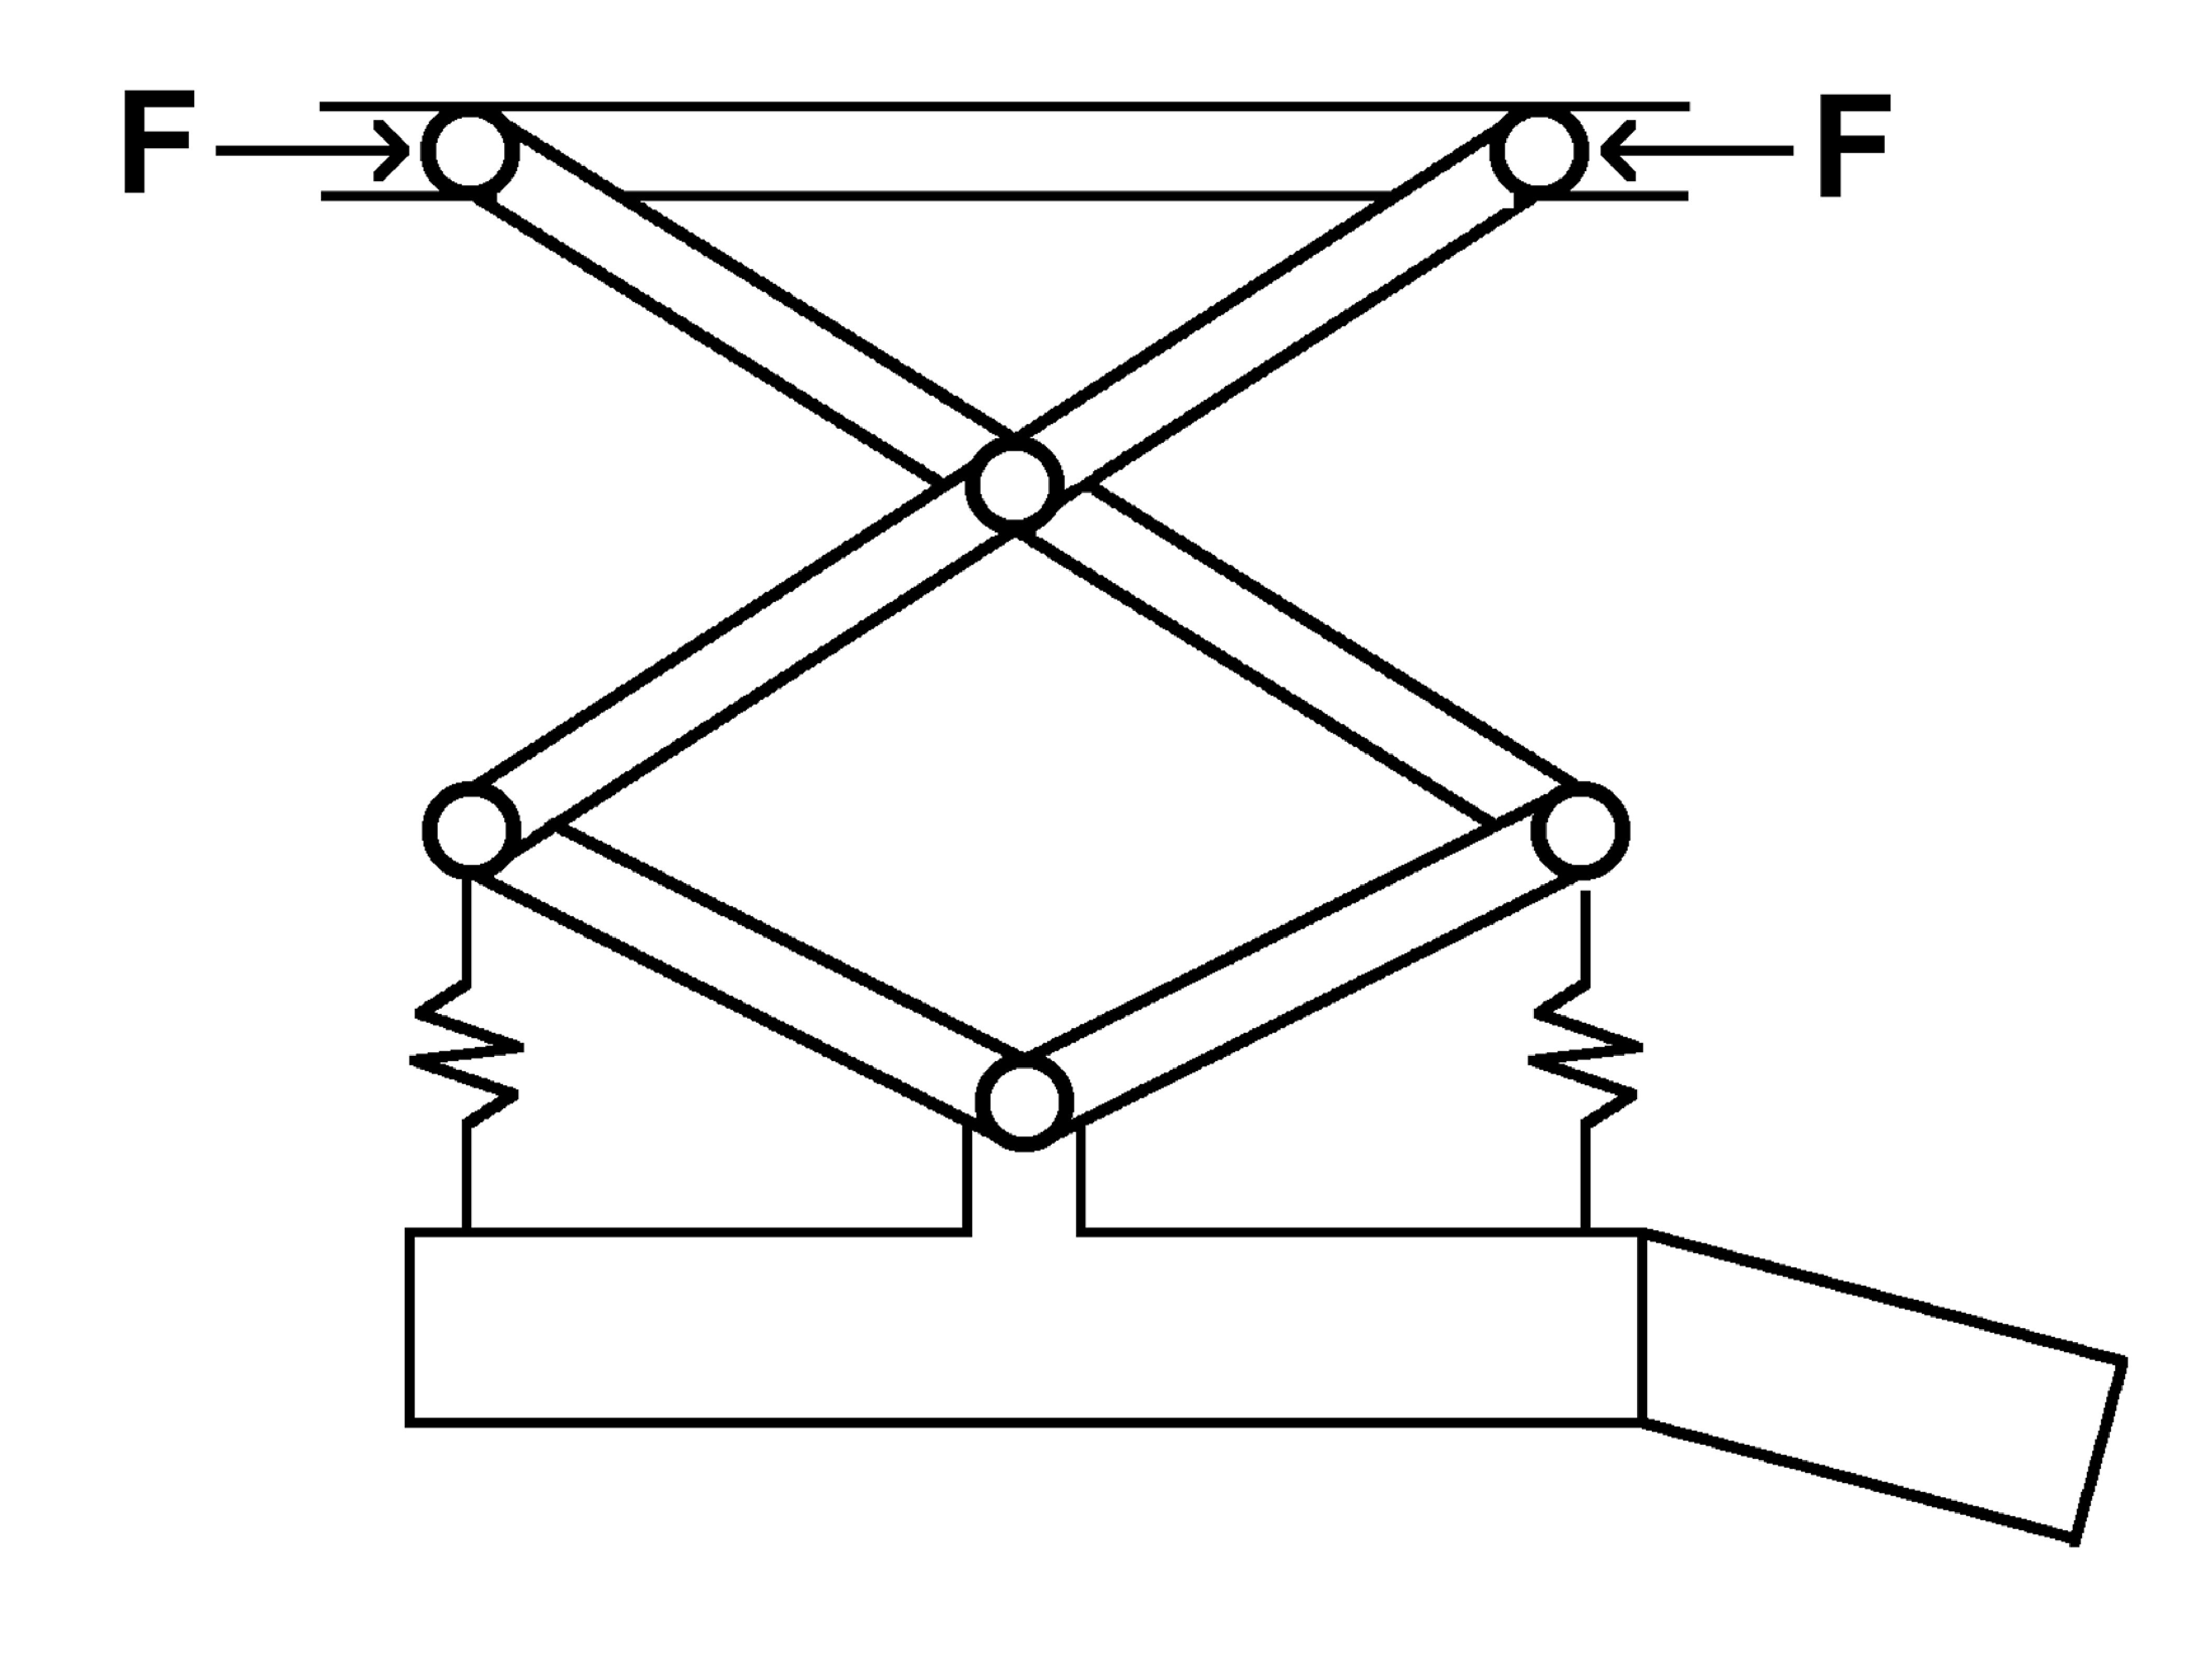
\includegraphics[height=\imageheight]{legDesign}
    					\caption{Diagrammatic representation of the pantograph mechanism used for AccoBot's legs}
    					\label{legDesign}
    				\end{multicols}
    			\end{figure}
    			\\
                \hspace*{2ex}The ratio between the longer base links of the pantograph and the tip links is 2:1, because this provides the maximum range of diameters for the smallest change in the base width\supercite{okada1987mogrer}.
				The required link length $L$ to allow AccoBot to adapt to the chosen range of diameters, 457.2 - 914.4 mm, can be found:
				\begin{align}
					r_{min} &= \frac{3L}{2} \sin \left( \theta_{min} \right) \label{rMin}
					\\
					r_{max} &= \frac{3L}{2} \sin \left( \theta_{max} \right)
					\\
					\implies \Delta r &= \frac{3L}{2} \left( \sin \left( \theta_{max} \right) - \sin \left( \theta_{min} \right) \right)
					\\
					L &= \frac{2 \Delta r}{3 \left( \sin \left( \theta_{max} \right) - \sin \left( \theta_{min} \right) \right)}
				\end{align}
				\\
                \hspace*{2ex}The pantograph has been designed to move from an angle of $\theta_{min} = 10^\circ$ to $\theta_{max} = 60^\circ$, spanning a change in radius of 228.6 mm, so the link length $L$ = 220.1 mm.
			
			\subsubsection{Required Forces} \label{requiredForce}
			
				It is important to consider the required maximum output of the linear actuators for AccoBot to operate in all pipes.
				This maximum force occurs when AccoBot is climbing vertically and must create enough normal force for friction to support its entire weight.
				This force can be calculated from \figref{legDiagram}:
				\begin{align}
					N &= \frac{2 F \tan \left( \theta \right)}{\cos \left( \phi \right)}
					\\
					F_f &= \mu_{t,p} N
					\\
					&= \frac{2 \mu_{t,p} F \tan \left( \theta \right)}{\cos \left( \phi \right)}
					\intertext{where $F_f$ is the frictional force on one track, and $\mu_{t,p}$ is the coefficient of friction between the tracks and the pipe. \newline In order for this to balance the weight W:}
					\begin{split}
						W &= 3 F_f
						\\
						&= \frac{6 \mu_{t,p} F \tan \left( \theta \right)}{\cos \left( \phi \right)} \label{maxWeight}
					\end{split}
					\\
					\implies F &= \frac{W \cos \left( \phi \right)}{6 \mu_{t,p} \tan \left( \theta \right)} \label{reqMaxNorm}
				\end{align}
				\\
                \hspace*{2ex}Using estimates from other papers for $\mu_{t,p}$, which suggest $\mu_{t,p} = $ 1.21\supercite{sato2011development} - 1.6\supercite{park2010normal}, allows a maximimum force estimate using a value of $\mu_{t,p} = $ 1.21.
				From \equationref{reqMaxNorm}, it is clear that the worst case scenario occurs in smooth sections, where $\phi$ is expected to be close to $0^\circ$, and in the smallest pipe diameter, which minimises $\tan \left( \theta \right)$.
				\\
                \hspace*{2ex}The linear actuators chosen were selected to have 200 N of force output and a potentiometer to measure actuator extension\supercite{rsproLinear}.
				Using \equationref{maxWeight}, reproduced below, values for the worst case scenario are estimated.
				\begin{align*}
					W &= \frac{6 \mu_{t,p} F \tan \left( \theta \right)}{\cos \left( \phi \right)}
				\end{align*}
				The greatest force is required when $\mu =$ 1.21\supercite{sato2011development}, $\theta = 10^\circ$ and $\phi = 0^\circ$, which gives a maximum weight constraint of 528.5 N = 53.9 kg.
				With a safety margin of 1.5 for the linear actuator output, limiting their output to 130 N, the maximum weight becomes 343.5 N = 35 kg which is still significantly larger than similar robots.
				These cost £121.46 - £132.02 each depending on quantity, but the lower price can be used as this is for 10 or more actuators, less than 2 robots.
				Thus the actuator cost for a single AccoBot would be £728.76, as 2 linear actuators are used for each leg, a total of 6.
				The overall weight of these 6 linear actuators would be 0.504 kg, which is negligible compared to the weight of most of the other components, as well as the estimated weight of the AccoBot shell.
				
			\subsubsection{Body Dimension Constraints}
			
    		    As the link length, $L$ = 220.1 mm, the minimum height of a leg is $r_{min}$ = 57.3 mm, from \equationref{rMin}, not including the tracks, which can be used to find the maximum body diameter $D_{r,max}$
    			\begin{align}
    				D_{r,max} = D_{pipe,min} - 2 \left(r_{min} + w_{track} \right)
    			\end{align}
    			Assuming a track width of $w_{track}$ = 70 mm, the body diameter $D_{r,max}$ = 202.5 mm, setting a constraint on the dimensions of the inner body based on the design criteria.
    			\\
                \hspace*{2ex}The minimum length of the body is set by the smallest distance the linear actuators need to be placed apart to function.
    			By considering the links at their flattest, the minimum distance between the linear actuators is $l_{min} = L \cos \left( \theta_{min} \right)$.
    			This sets the body minimum length $l_{min}$ =  216.8 mm, ignoring the length of the linear actuators.
    			While this is a generous estimate, the constraint of the maximum length is of greater concern.
    			\\
                \hspace*{2ex}Maximum body length $l_{max}$ is constrained by the ability of AccoBot to turn corners inside the pipe, and it is necessary to consider how this compares to the minimum to make sure there is a suitable range to work with.
    			The smallest pipe diameter $D_{pipe,min}$ = 457.2 mm gives the worst case scenario, and the curvature radius $r_c = \frac{3}{2} D_{pipe}$\supercite{roh2005differential} = 685.8 mm.
    			As the robot diameter $D_{r,max} \nless \left( 2 \sin \left( 45^\circ \right) - 1 \right) D_{pipe,min}$ the maximum length can be found from the following equation\supercite{roh2005differential}:
    			\begin{align}
    				l_{max} &= 2 \sqrt{4D_{pipe}^2 - \left( D_{pipe} + D_{r,max}\right) ^ 2}
    				\\
    				&= 1266.3 \ \mathrm{mm} \notag
    			\end{align}
    			% Makes max volume 187*10^6 mm^3
			
			\subsubsection{Active Compliance Joint} \label{trackDetails}
			
				The tracks use an active compliance joint, as shown in \hyperref[activeCompliance]{Figures \ref*{activeCompliance} \& \ref*{unevenBehaviour}}, which allows for AccoBot to maintain maximum surface contact at all times.
				The active compliance joint consists of a torsional spring and radio-controlled servo motor, which are both attached around the same axis.
				The servo motor is attached to the rear tracks, and the spring is attached between the front track and the servo motor itself.
				\\
                \hspace*{2ex}When AccoBot passes over an uneven surface, the servo motor forces the front track down, maintaining contact with the pipe wall, as shown in \hyperref[unevenBehaviour]{Figure \ref*{unevenBehaviour}(a)}.
				If instead AccoBot is in a section where the pipe wall is concave, the torsional spring will allow it to fold, shown in \hyperref[unevenBehaviour]{Figure \ref*{unevenBehaviour}(b)}, and maintain contact with as much of the wall as possible.
				The active compliance joint also includes an angular encoder to return the track bend angle, which is used in \sectref{complianceControl}.
				\begin{figure}[h]
					\centering
					\begin{multicols}{2}
						\includegraphics[height=\imageheight]{activeCompliance}
						\caption{Function and construction of an active compliance joint. Figure from \cite{park2010normal}}
						\label{activeCompliance}
						\columnbreak
						\includegraphics[height=\imageheight]{unevenBehaviour}
						\caption{Behaviour of active compliance joint over uneven surfaces (travelling upwards). Figure from \cite{park2010normal}}
						\label{unevenBehaviour}
					\end{multicols}
				\end{figure}
				\\
                \hspace*{2ex}For the track module, the best reference point was the Inuktun Minitrac, a larger version of the Inuktun Microtrac module used by Ciszewski et al.\supercite{ciszewski2015design} for their testing of a pipe inspection robot.
				These cost £7,900 each, and three are required for each leg of AccoBot, bringing the overall cost to £71,100.
				However these modules are over specified, as each has a pull rating of roughly 30 kg for continuous duty\supercite{inuktunTracks}, meaning AccoBot can weigh up to 270 kg, which would be an unrealistic and impractical figure.
				Each module can be provided in either aluminium, brass or steel, with the main difference being the weight.
				Aluminium was chosen, as it is the lightest of the three, and each module weighs 5.7 kg, so all 9 track modules weigh 51.3 kg in total.
				As this is much larger than the maximum weight constraint from the linear actuators, a different design should be considered, with a motor driving the tracks instead, which can be carefully designed to minimise the weight.
				Additionally, the Minitrac is no longer sold for commercial uses, as Eddyfi Technoloiges, who manufacture the component, found that they were often being used in products which compete with their own pipe inspection robots.
				However, these track modules give an indication of the eventual cost to expect for AccoBot if using prebuilt modules.
				
			\subsubsection{Leg Rotation}
				
				The rotation of the two legs relative to the body of AccoBot uses a single motor at each end, driving two planetary gear systems in opposite directions.
				The motor drives the sun gears of two planetary gear systems, shown in \figref{planetaryDrive}, which rotate in opposite directions to keep the robot symmetrical.
				The direction is reversed for the planetary drive not adjacent to the driving motor using a small differential gearbox, shown in \figref{diffGearbox}, which allows for compact motion reversal.
				These allow the legs to move around the body, from almost directly below AccoBot to a horizontal plane at $90^\circ$ to the top leg.
				\begin{figure}[h]
					\centering
					\begin{multicols}{2}
						\includegraphics[height=\imageheight]{planetaryDrive}
						\caption{Planetary drive used to move the legs relative to the main body}
						\label{planetaryDrive}
						\columnbreak
						\includegraphics[height=\imageheight]{diffGearbox}
						\caption{Differential gearbox for coaxial rotational direction reversing}
						\label{diffGearbox}
					\end{multicols}
				\end{figure}
				\\
                \hspace*{2ex}As both legs are driven from the same motors, both legs are symmetrical at all times, and the leg position can be summarised by a single leg rotation angle $\lambda$, measured from the top leg, which varies from $\lambda = 90^\circ$ to $\lambda = 150^\circ$ for AccoBot.
				This rotation allows AccoBot to adapt to different pipe inclinations.
				It will be quicker to drive along horizontal pipes with the almost vertical drive system, but when climbing vertical pipes a more even distribution of contact points is preferred, most likely using $\lambda = 120^\circ$.
				\\
                \hspace*{2ex}The motor used for rotation of the legs relative to the body has no torque requirement, as an experimental result would be required, but a high torque motor would be ideal.
				A sample product which is both relatively small and high torque was selected\supercite{rsproRotation} as it has a maximum output torque, at stall, of 1.46 Nm.
				The diameter of the motor is 42.8 mm, meaning that there is plenty of space to use a larger, more powerful motor if testing suggests it is necessary.
				The drives cost £141.84 per motor, and 2 are required for a single AccoBot.
				Since similar motors are required as RC servo motors for the active compliance joint, another 3 would be included in AccoBot, bringing the total cost for 5 motors to £709.20.
				\\
                \hspace*{2ex}The weight of the major manufactured components of the locomotion system were estimated using the 3D CAD models, shown in \hyperref[gearCAD]{Figures \ref*{gearCAD}, \ref*{shortLinkCAD} \& \ref*{longLinkCAD}} to estimate their volume.
				The leg links were assumed to be made out of stainless steel, and the gear was to be made of aluminium.
				\begin{figure}[h]
					\centering
					\begin{multicols}{3}
						\includegraphics[height=0.18\textwidth]{gearCAD}
						\caption{Aluminium gear used as the outside of the planetary gear, with dimensions}
						\label{gearCAD}
						\columnbreak
						\includegraphics[height=0.18\textwidth]{shortLinkCAD}
						\caption{Stainless steel short link of the leg mechanism with dimensions}
						\label{shortLinkCAD}
						\columnbreak
						\includegraphics[height=0.18\textwidth]{longLinkCAD}
						\caption{Stainless steel long link of the leg mechanism with dimensions}
						\label{longLinkCAD}
					\end{multicols}
				\end{figure}
				\\
                \hspace*{2ex}The density of stainless steel is 7900 kg m\textsuperscript{-3}\supercite{HLT}, so the longer link weighs 0.653 kg and the shorter link weighs 0.350 kg.
				Thus, a single leg, made of 2 of each link, weighs 2 kg, bringing the total contribution of the three legs to 6 kg for the whole robot.
				The density of aluminium is 2700 kg m\textsuperscript{-3}\supercite{HLT}, which makes the weight of a single gear 1.71 kg, and there are 4 inside AccoBot, bringing the total weight up to 6.84 kg.
				This needs to be mitigated by refining the design, which was mainly created for visual purposes, and is thicker than would be necessary in reality.
			
		\subsection[Internal Sensing]{Internal Sensing - Montgomery Beresford}
		
		AccoBot requires multiple internal sensors in order to understand and navigate its environment; this section discusses their use and selection.
		
		\subsubsection{Angular Sensors}
            		
       For the angular sensors, whose use are described in \sectref{Lomcotion}, magnetoresistive sensors and Hall effect sensors were investigated. The benefits of magnetoresistive sensors are that they are highly accurate, are not sensitive to noise caused by external vibrations, are very small and are energy efficient. However, they do not always measure 360 degrees rotations and can be sensitive to temperature fluctuations. Meanwhile, Hall effect sensors have the advantage of being able to measure 360 degrees of motion, but they are not as accurate as magnetoresistive sensors. Since in this application accuracy is the most important factor and 360 degrees measurement is not required magnetoresistive sensors are used.
           \begin{floatingfigure}[r]{0.6\textwidth}
					\centering
					\includegraphics[width=0.57\textwidth] {AMR_comparison table_formatted}
					\captionof{table}{Table comparing different angular encoders}
					\label{rotary_encoders_comparison}
			\end{floatingfigure}
            \hspace*{2ex}There are three main types of magnetoresistive sensors: anisotropic magnetoresistive sensors (AMR), tunnel- magnetoresistive sensors (TMR) and giant magnetoresistive sensors (GMR) which are compared in \tableref{rotary_encoders_comparison} compares them.
            \begin{floatingfigure}[r]{0pt} \end{floatingfigure}
\hspace*{2ex}TMR sensors were chosen because they have less age deterioration and less temperature drift than AMR and GMR sensors, meaning they are more accurate and because accuracy is the most important factor in this consideration. They are also the most sensitive which provides greater resolution.
            %For the angular sensors, whose use are described in \sectref{Lomcotion}, magnetoresistive sensors and hall effect sensors were investigated. 
         %   The benefits of magnetoresistive sensors are that they are highly accurate, not sensitive to noise caused by external vibrations, very small and are energy efficient.
      %      However they do not always measure 360 rotations and can be sensitive to temperature fluctuations. 
         %   Meanwhile Hall effect sensors have the advantage of being able to measure 360 degrees of motion but they are not as accurate as Magnetoresistive sensors. 
      %      Since in this application accuracy is the most important factor and 360 degrees motion is not required magnetoresistive sensors are used.

         %   There are three main types of magnetoresistive sensors that had to be considered.
          %  These are anisotropic magenetoresistance sensors (AMR), tunnel-magentoresistance sensors (TMR) and giant magnetoresistance sensors (GMR).
            
		    %\begin{floatingfigure}[r]{0pt} \end{floatingfigure}
            
           % \tableref{rotary_encoders_comparison} compares them where MR is the magnetoresistance ratio, which describes how sensitive the sensor is to changing its electrical resistance with changes in external magnetic fields.\supercite{magnetoresistance}
         %  TMR sensors are made of three layers, the ferromagnetic free layer, the insulator barrier layer and the ferromagnet pin layer.\supercite{Tunnel_magnetoresistance} 
          %  The free layer changes its magnetic orientation to align with externally applied magnetic fields whilst the pin layer has its magnetic orientation in a constant direction.
         %   This means that when the externally applied magnetic field is aligned in parallel with the magnetic field of the pin layer there is low resistance and therefore large current, but as the external magnetic field changes direction, due to rotation, so that it is becomes more anti-parallel to the pin layer’s magnetic field the resistance increases. 
       %     The changes in current that this causes are detected, and thus rotation is detected.\supercite{explanation_magntoresistance1} 
        %    GMR sensors are very similar to TMR sensors however the current in GMR sensors flows parallel to the layers whereas in the TMR sensors it flows perpendicularly across it.
      %      For GMR sensors there is a change in resistance due to electron scattering that is dependent on the spin orientation of the atoms within the ferromagnetic layers, this technique is less sensitive than that used in the TMR.
            
       %     AMR sensors on the other hand only have one layer of permalloy. 
        %    Changes in resistance in AMR sensors vary depending on the material, but largely it is due to changes in spin-dependent scattering.\supercite{explanation_magntoresistance2}
       %     The anisotropic effect that is used in AMR sensors is the dependence of resistance on the angle between the electric current and the external magnetic field.
            
       %     Between these TMR was chosen because it has less age deterioration and temperature drift than the other two.
       %     This is important when the accuracy is the most important factor. 
      %      Furthermore, it can be seen from \tableref{rotary_encoders_comparison} that TMR sensors are the most sensitive, which provides greater resolution. What is more, because it produces a high output, it does not require extra amplification, reducing cost and complexity. 
            
       %     In particular the ASR022ABZ Noncontact TMR Encoder Sensor was chosen because it provides all the necessary performance for an appropriate price and weight.

				
	%						\begin{floatingfigure}[r]{0.5\textwidth}
	%		\centering
	%			\includegraphics[width = 0.47\textwidth]{overviewCADLabels}
	%			\caption{3D CAD model of AccoBot with major components labelled}
	%			\label{3DSketch}
	%		\end{floatingfigure}
	%	
		%	    \begin{figure}[h]
		%			\centering
		%%			\caption{Sensitivity of different angular encoders \cite{TMR_graph}}
		%			\label{rotary_encoders_graph}
		%		\end{figure}
            
            \subsubsection{Comparison of AHRS, IMU and INS}

            AccoBot needs to be able to determine its orientation so that it can calculate its pose, as described in \sectref{poseCalculation}. This information is fed into the localisation system as well as the navigation control system. Three options were considered to provide this information, an attitude heading reference system (AHRS), an inertial measurement unit (IMU) and an inertial navigation system (INS). \tableref{AHRS_comparison} shows the comparison of these.
            \\
            \hspace*{2ex}The main consideration for this was providing as accurate information as possible since the accuracy of the robot’s systems is highly dependent on the accuracy of its knowledge of its pose. It was decided to use the AHRS because it provided attitude values and suffers less drift than the IMU due to its application of a Kalman filter. The INS's expense is not justified as it is only more accurate when GNSS data is available, which it is not. %is more expensive but can provide more accurate information if regular GNSS information is available. However, this is not available, therefore the extra expense would not be justified. 
             In particular the Ellipse 2 Micro AHRS was picked. This was because it is light and compact, with a weight of 10g and size of 26.8 $\times$ 19.8 $\times$ 9.5 mm\supercite{Ellipse_Ahrs}.
         %   The robot needs to be able to determine its orientation so that it can calculate its pose, as described in \sectref{poseCalculation}.
     %       This information is fed into the localisation system as well as the navigation control system. 
       %     Three options were considered to provide this information, an attitude heading reference system (AHRS), an inertial measurement unit (IMU) and an inertial navigation system (INS). \tableref{AHRS_comparison} shows the comparison of these.
       %     The main consideration for this is providing as accurate information as possible since the accuracy of the robots systems is highly dependent on the accuracy of its knowledge of its pose. 
     %       It was decided to use the AHRS because it provided attitude values and suffers less drift than the IMU due to its application of a Kalman filter. 
      %      The INS is more expensive but can provide more accurate information if regular GNSS information is available. 
      %      However this is not available, therefore the extra expense would not be justified. For this reason an AHRS was chosen to be used.
       %     In particular the Ellipse 2 Micro AHRS was picked.
       %     This was because it is light and compact, with a weight of 10g and size of 26.8 x 19.8 x 9.5 mm.\supercite{Ellipse_Ahrs}
            \begin{table}[h]
					\centering
					\includegraphics[width=0.8\textwidth]{ahrs comparison in pounds.png}
					\caption{Table showing that an AHRS would be the best choice out of the IMU, AHRS and INS. Prices from \cite{Ellipse_Ahrs}}
					\label{AHRS_comparison}
				\end{table}
			%	   \begin{table}
		%			\centering
		%				\includegraphics[width=0.47\textwidth] {AMR_comparison table_formatted}
		%				\caption{Table comparing different angular encoders}
		%				\label{rotary_encoders_comparison}
		%	\end{table}
			%\begin{table}[h]
					%\centering
					%\begin{multicols}{2}
					%	\centering
					%\includegraphics[width=0.7\textwidth]{IMU_formatted_table}
					%\caption{Table showing that an AHRS would be the best choice out of the IMU, AHRS and INS. Prices %from \cite{Ellipse_Ahrs}}
			%		\label{AHRS_comparison}
			%			\columnbreak
			%			\includegraphics[width=0.3\textwidth] {AMR_comparison table_formatted}
			%			\caption{Table comparing different angular encoders}
			%			\label{rotary_encoders_comparison}
			%		\end{multicols}
			%	\end{table}
				
        \subsubsection{Odometers}
        
         Physical odometers are required to pass information into the localisation system about how far the robot has travelled. Although these suffer drift, as described in \sectref{localisationSection}, they provide useful extra information for producing an accurate overall system.
          %  \hspace*{2ex}One odometry method would be to use the relation between the motor power and track speed. Despite this being the least complex and cheapest solution, its lack of accuracy due a nonlinear and unpredictable relationship between power and the motor means this method will not be used.
            \\
            \hspace*{2ex}Wheel rotary odometers provide information about the speed of the robot from which the distance travelled can be derived hence providing a solution that lacks complexity and is cheap.% By integrating the speed of AccoBot over time displacement could be calculated. Such a method however can incur errors such as the tracks slipping which can lead to odometer drift, which is why they could not be used as the only input for localisation.
            \\
            \hspace*{2ex}For these odometers there was the option of using encoders or resolvers. Resolvers provide an analogue signal that corresponds to the absolute position of the object, whereas encoders use digital pulses to measure the amount of rotation\supercite{Encoder_resolver}. Resolvers were decided against due to their complexity and lower speed range. Relative encoders were chosen instead of absolute encoders because only the relative shaft position will need to be known.
            \\
            \hspace*{2ex}Of these encoders there were three main types of encoders to be considered: magnetic, optical and capacitive. Magnetic encoders have the advantage of being more robust and not as sensitive to environmental contamination as optical sensors, however, they are often not as accurate. %Further, they can suffer interference from electrical motors and since the electrical motors in the tracks will be in close proximity to the encoders this would be a significant factor. 
            \\
            \hspace*{2ex}Optical encoders have a much higher accuracy\supercite{Encoders}, however, they consume more power and are more likely to break due to the LEDs present\supercite{Encoders}. Since the effectiveness of the localisation is affected by the effectiveness of its odometers, this risk of failure of the odometer has high significance. 
            \\
            \hspace*{2ex}Capacitive encoders have greater robustness, and do not consume as much power due to not using an LED. Capacitive encoders are also more compact than optical and magnetic encoders and are less expensive\supercite{Encoders}. These factors are considered in \tableref{odometer_comparison}, leading to capacitive encoders being selected for use. %These arguments were considered and quantified into three separate metrics, robustness, accuracy and resolution\footnote{Due to the relative inexpense of the encoders compared to other parts of AccoBot, cost was not considered to be a factor worth considering.}, and each given their own weighting. \tableref{odometer_comparison} compares these metrics from this it was decided to use capacitive encoders.
            Specifically, the AMT31 Series encoders, which cost £6 each and weigh 15.7g, were chosen because they provide the necessary performance for a good price and weight. 
                
	      %  Physical odometers are required to pass information into the localisation system about how far the robot has travelled. Although these suffer drift, as described in \sectref{localisationSection}, they provide useful extra information for producing an accurate overall system.
	      %  For this magnetic, optical and capacitive encoders were considered, from whose speed measurement distance travelled can be derived.
         %   \\
         %   \hspace*{2ex}
         %   Magnetic encoders have the advantage of being more robust and not as sensitive to environmental
         %   contamination as optical sensors, however, they are often not as accurate. Further, they can suffer interference from electrical motors and since the electrical motors in the tracks will be in close proximity to the encoders this would be a significant factor. 
         %   \\
         %   \hspace*{2ex}Optical encoders have a much higher accuracy\supercite{Encoders}, however, they consume more power and are more likely to break due to the LEDs present\supercite{Encoders} Since the effectiveness of the localisation is affected by the effectiveness of its odometers, this risk of failure of the odometer has high significance. 
           % \\
        %    \hspace*{2ex}Capacitive encoders have greater robustness, and do not consume as much power due to not using an LED. 
        %    Capacitive encoders are also more compact than optical and magnetic encoders and are less %expensive\supercite{Encoders}. These arguments were considered and quantified into three separate metrics, robustness, accuracy and resolution\footnote{Due to the relative inexpense of the encoders compared to other parts of AccoBot, cost was not considered to be a factor worth considering.}, and each given their own weighting. \tableref{odometer_comparison} compares these metrics from this it was decided to use capacitive encoders. Specifically, the AMT31 Series encoders, which cost £6 each and weigh 15.7g, were chosen because they provide the necessary performance for a good price and weight. 
          %  \hspace*{2ex}One odometry method would be to use the relation between the motor power and track speed. Despite this being the least complex and cheapest solution, its lack of accuracy due a nonlinear and unpredictable relationship between power and the motor means this method will not be used.
           % \\
         %   \hspace*{2ex}Wheel rotary odometers provide information about the speed of the robot and provide a solution that lacks complexity and is cheap. By integrating the speed of AccoBot over time displacement could be calculated. Such a method however can incur errors such as the tracks slipping which can lead to odometer drift, which is why they could not be used as the only input for localisation.
           % \\
       %     \hspace*{2ex}For these odometers there was the option of using encoders or resolvers. Resolvers provide an analogue signal that corresponds to the absolute position of the object, whereas encoders use digital pulses to measure the amount of rotation.\supercite{Encoder_resolver} Resolvers were decided against due to their complexity and lower speed range. Relative encoders were chosen instead of absolute encoders because only the relative shaft position will need to be known.
           % \\
     %       \hspace*{2ex}Of these encoders there were three main types of encoders to be considered: magnetic, optical and capacitive.
            
           % Magnetic encoders have the advantage of being more robust and not as sensitive to environmental contamination as optical sensors, however, they are often not as accurate. Further, they can suffer interference from electrical motors and since the electrical motors in the tracks will be in close proximity to the encoders this would be a significant factor. 
            %\\
         %   \hspace*{2ex}Optical encoders have a much higher accuracy\supercite{Encoders}, however, they consume more power and are more likely to break. LEDs in these encoders can burn out after 10,000 to 20,000 hours of use.\supercite{Encoders} Since the effectiveness of the localisation is affected by the effectiveness of its odometers, this risk of failure of the odometer has high significance. 
            %\\
       %     \hspace*{2ex}Capacitive encoders have greater robustness, and do not consume as much power due to not using an LED. They require 6 to 10mA of current compared to 20 to 50 mA required by optical encoders. Capacitive encoders are also more compact than optical and magnetic encoders and are less expensive\supercite{Encoders}. These arguments were considered and quantified into three separate metrics, robustness, accuracy and resolution\footnote{Due to the relative inexpense of the encoders compared to other parts of AccoBot, cost was not considered to be a factor worth considering.}, and each given their own weighting. \tableref{odometer_comparison} compares these metrics from this it was decided to use capacitive encoders. Specifically, the AMT31 Series encoders, which cost £6 each and weigh 15.7g, were chosen because they provide the necessary performance for a good price and weight. 
            %From this decision table it was decided to use a capacitive odometer and specifically to use the AMT31 Series which cost £6 each and weight 15.7g because it again provided the necessary performance for a good price and weight.
	     %   Physical odometers are required to pass information into the localisation system about how far the robot has travelled.
	      %  These suffer drift, as described in \sectref{localisationSection}, but they provide extra information that is used to produce a more accurate overall system.
	       % One odometry method would be to use the relation between the motor power and track speed.
	        %This would have the benefit of not requiring any extra sensors and would therefore be the cheapest and least complex solution.
	        %However its accuracy would be too low due to the non-linear relationship between the power and the motor that would be dependent on that angle the robot is travelling, the weight of the robot, and the coefficient of friction between the robot and ground, among other things, all of which would vary.
	       % For this reason this method would not be used.
	        %Wheel rotary encoders are another solution that lacks complexity and is cheap.
	        %The use of the robots clock and $s=ut$ would allow the displacement to be calculated. 
	        %Such a method however can incur errors such as the tracks slipping which can lead to odometer drift, and can therefore not be used as the only input for localisation.
	        %For these odometers there was the option of using encoders or resolvers. Resolvers provide an analogue signal that corresponds to the absolute position of the object, whereas encoders use digital pulses to measure the amount of rotation.\supercite{Encoder_resolver}
	        %Resolvers were decided against due to their complexity and lower speed range.
	        %For the encoders there was an option to use relative or absolute encoders. 
	        %Absolute encoders were found to not be required since it is only the relative shaft position that would need to be measured.
	        %There were three main types of encoders to consider: magnetic, optical and capacitive.
	        %Magnetic encoders have the advantage of being more robust and not as sensitive to environmental contamination as optical sensors, however, they are often not as accurate. 
	       % Further, they can suffer interference from electrical motors and since the electrical motors in the tracks will be in close proximity to the encoders this would be a significant factor.
	        %Optical encoders have a much higher accuracy\supercite{Encoders}, however, they consume more power and are more likely to break. LEDs in these encoders can burn out after 10,000 to 20,000 hours of use.\supercite{Encoders} 
	        %Since the effectiveness of the localisation is highly affected by  the effectiveness of its odometers, this risk of failure of the oometer has high significance.
	        %Capacitive encoders have greater robustness, and do not consume as much power due to not using an LED. 
	        %They require 6 to 10mA of current compared to 20 to 50 mA required by optical encoders.
	        %Capacitive encoders are also more compact than optical and magnetic encoders and are less expensive\supercite{Encoders}. 
	        %They have a downside of being prone to electrical interference, however modern packages housing the encoders make this less significant than the noise that the other encoders face.\supercite{Encoders}
	        %\tableref{odometer_comparison} compares the metrics that need to be considered when choosing which type to use. 
	        %Due to the relative inexpense of these compared to other parts of the robot, cost was not considered to be a factor worth considering. 
	        %From this decision matrix it was decided to use a capacitive odometer.
	       % It was decided to specificallu use the AMT31 Series which cost £6 each and weight 15.7g because it again provided the necessary performance for a good price and weight.
	        \begin{table}[h]
    			\centering
    			\includegraphics[width=0.8\textwidth]{Encoder comparison table}
    			\caption{Comparison of the different types of odometers, highlighting capacitive are best}
    			\label{odometer_comparison}
			\end{table}			
	  %Having chosen the types of sensors here the specific components will be specified. The angular sensor is a TMR sensor in particular the ASR022ABZ Noncontact TMR Encoder Sensor was chosen. This is because it provides all the necessary performance for an appropriate price and weight. The odometer encoder was chosen for similar reasons. It was decided to use the AMT31 Series which cost £6 each and weight 15.7g. For the AHRS the Ellpise 2 Micro was chosen due to its small size and weight combined with its reported high quality. For the EMAT sensor the Oympuse EMAT E110-SB was chosen because it comes with software and appropriate interfaces to process the data that it collects.
       	%	In particular the Ellipse 2 Micro AHRS was picked.
           %  This is because it is light and compact. It has a weight of 10g and size of 26.8 x 19.8 x 9.5 mm.\supercite{Ellipse_Ahrs}
       	  		%\begin{table}[H]
       	  		%\centering
       	  		%\includegraphics[scale=0.7]{smaller component sensor table}
       			%	\caption{Costs and weights of sensor hardware}
       			%	\label{sensorHardware}
       			%\end{table}				
	        
	        \subsection[Damage Sensing]{Damage Sensing - Montgomery Beresford}
	        
	     For the robot to solve the problems discussed in \sectref{solutionEvaluation} it must be able to identify damage within the pipes.
	        AccoBot will be primarily used in cast iron pipes, within which corrosion and cracks are the major categories of damage found\supercite{Failure_pipes}\supercite{Failure_pipes2}.
	        AccoBot will also need to provide information about the location of connecting pipes, joints, valves and other objects within the pipes, so a detection system that can do both would be useful.
	        \\
            \hspace*{2ex}In order to determine how to detect the damage three main steps were used. 
	        Firstly determining the type of sensor to use and therefore the type of data that will be processed. 
	        Secondly, having determined the type of sensor, looking into the best types of that type of sensor, which is discussed in \sectref{visualSensors}.
	        Finally, investigating how to best process the data provided by the sensor so as to extract the desired information, which is discussed in \sectref{featureDetection}.
	       \\\hspace*{2ex}
	        When assessing the type of sensor to be used to detect damage in the pipes the constraints of the application as well as the desired outcomes must be considered.
            The robot must be able to adapt to different diameter pipes since it would be inspecting pipes of varying diameters.
	        Secondly, it is important to maximise the amount of valuable information that can be gained from a job due to the relatively high costs and disruption created by accessing the pipes.
	        For this reason also the method of inspection should allow the robot to move quickly through the pipes. 
	        Finally, the inspection method should be able to be used on cast iron, steel and PE pipes. 
	
	   \textbf{Type of Damage Sensors}\label{damagesensors}
	        
        When deciding on what technique to use to detect damage, and therefore what type of sensor is required, metrics would ideally be looked at to determine the accuracy of these techniques in the environment that the robot will be in. This would involve creating a rig to test the different techniques and then looking at their false positives, false negatives, recall and sensitivity ratios. However, since the robot is not constructed and there is currently no access to these environments this is not possible,  which means that the decision was made from an analysis of the technology, as is discussed below. PipeDream looked at magnetic flux leakage, piezoceramic ultrasonic transducer detection, electromagnetic acoustic transducers, visual sensing and laser scanning as potential techniques.
        \\\hspace*{2ex}
	        \textbf{Magnetic Flux Leakage (MFL)} uses an array of sensors placed on arms in a circular configuration. The array has magnets that produce a magnetic field that flows through the pipes between the poles of each arm of the array. A flux sensor is placed between the poles of the magnets and detects variation in the flux due to damage and stress. This flux increases for tensile stresses and decreases for compressive stresses\supercite{MFL_explanation}.
	        \\
            \hspace*{2ex}This type of detection is beneficial because it can detect stresses in the material which might predict damage in the future and it can detect damage within the pipe wall. It is also less sensitive to surface conditions compared to ultrasonic detection which is useful when considering that there may be dirt build up on the walls.
	        \\
            \hspace*{2ex}However, MFL requires a constant, small gap between the sensors and the sides of the walls\supercite{MFL_explanation}. To solve this it was considered designing a mechanism which had the detectors on extendable arms that could adapt to the pipe diameter. However, the circular geometry required for this technique added a large amount of complexity which would introduce greater cost and weight to AccoBot. Another downside of MFL, is that corrosion products can build up on the magnets which decreases its accuracy and it can only be used with ferromagnetic pipes. Comparing this to the desired criteria meant that it was decided not to use MFL. 
	        \\\hspace*{2ex}
	        \textbf{Piezoceramic Ultrasonic Transducer Detection (PUT)} is a method that measures the time it takes for an emitted ultrasonic pulse to return to the sensor having reflected off a medium boundary\supercite{UT_explanation}. This sensor is usually a piezoceramic transducer\supercite{UT}, which, by sending and receiving short pulses of ultrasounde, can detect internal flaws in the pipe\supercite{Corrosion}. It can detect these flaws at higher accuracy and greater depths into the wall than MFL\supercite{MFL_Pig}.
	        \\
            \hspace*{2ex}However, PUT detection requires a couplant fluid between the sensor and the wall\supercite{UT_explanation}. This would make it difficult to adapt to different diameters and would require the robot to be supplied with a fluid, something that would reduce its range considerably, and it would not be desirable to introduce a foreign fluid into live gas pipes. Furthrmore, it needs to be calibrated with the thickness of the pipe which, in a pipe system in which there is imperfect information and the pipe thickness changes as the diameter changes, makes PUT not feasible.
	       \\\hspace*{2ex}
	       % \textbf{Eddy Current Testing (ECT)} uses a probe that produces an alternating magnetic field using an electromagnet. This induces an eddy current in the wall of the pipe. The eddy current is then measured, providing information about the integrity of the wall\supercite{ECT}. ECT has the benefit of being non-contact\supercite{Corrosion}, and it has an advantage over MFL because it can be used in both ferromagnetic and non-ferromagnetic material for surface inspection. However, ECT is more sensitive to differing permeability of the wall than MFL and the data is therefore harder to interpret\supercite{MFL_explanation}. Besides this, ECT is another technique which requires the sensor to be in close proximity to the wall which would make it hard to adapt to different diameters, therefore, it was decided against\supercite{ECT}.
	        \\\hspace*{2ex}
	        \textbf{Electromagnetic Acoustic Transducers (EMAT)} are used in a non-contact ultrasonic testing technique that does not require a couplant. The EMAT works by using magnetic fields to induce ultrasonic waves into the wall of the pipe. The waves that go through the pipe wall and when they return induce a current in the EMAT’s receiving coil\supercite{EMAT}. EMAT can be used to provide information about wall loss due to damage such as corrosion\supercite{EMAT}, and also about defects within the walls which is a major advantage. Its downside is that on AccoBot it will only be able to be deployed at certain angles and will miss out on damage over the majority of the circumference of the pipe. For this reason it cannot be used alone.
	        \\\hspace*{2ex}	
			\textbf{Visual Sensing} uses computer vision techniques to visually identify damage to the interior of the pipe. The main benefits of this are that the information produced is easy to interpret and the data collection can occur at a faster pace than with other methods. Moreover, the camera equipment required for it is relatively simple and inexpensive and would be required for the detection of objects anyway. Furthermore, visual detection can be used with a wide range of diameters since the camera does not need to be in close proximity with the wall and it can also be used with any pipe material. Its downsides are that it is has lower precision, its ability to accurately detect damage can be affected by lighting conditions and build up of dirt on the surface of the pipes, and that it cannot detect internal defects in the pipe. Despite this, its adaptability to the different pipe environments means that it was taken forward for further consideration. 
	\\\hspace*{2ex}	
	        \textbf{Laser Scanning} can provide higher resolution information about the inner surface of pipes than visual sensing. It allows the depth of pits and cracks, and the integrity of different sections of the pipe to be determined. From this information a laser scanner allows the client to know what the remaining life of the asset is and what the risk of leakage is\supercite{2g_robotics}. In addition to this laser scanners can be used for a range of pipe diameters so are adaptable. The downside of laser scanners compared to visual sensing is that it is a slow process to acquire detailed high-resolution information. It allows for an average rate of inspection of 6.1 cm of pipe length per minute\supercite{2g_robotics}\footnote{For a 0.91 metre diameter pipe it was calculated that AccoBot would need to stop every 0.37m and carry out a 360 degree scan that takes 6 minutes. This scan covers 0.466m along the axis of the pipe There is overlap on each of the scans.}. The laser scanner therefore offers the opportunity to provide more detailed information about the pipes than visual sensing, but because of its speed of acquiring data it cannot be used continuously over a large distance.
	        
	        \textbf{Conclusion}
	        \\
            Based on this discussion and analysis it was decided that the robot will use a combination of laser scanning, visual detection and EMAT sensors. The visual detection will allow the robot to move more quickly through the pipe where there is not as much damage, saving time and providing extra range. The EMAT sensors can be deployed when that data is desired by the GDC to provide information for their risk models. They will be placed on the side of each of the tracks, close to the wall. There are two modes for which the laser will be activated to extract data of greater resolution data. These are once the visual system detects damage above a certain threshold and the other is when it detects a joint. This threshold will be decided after test runs are done with the partnered company and will be adapted based on the difference risk preferences of the different clients.
            \\
            \hspace*{2ex}This visual detection system provides constraints on the processing of images. AccoBot moves at 0.1ms\textsuperscript{−1}, which means that if the robot were to process an image every 1 cm, AccoBot must be able to process images at 10 FPS. Therefore visual detection algorithms were chosen in \sectref{visual} to have as small as classification time as possible.
	 %       \textbf{Magnetic Flux Leakage (MFL)}
	  %      Magnetic Flux Leakage uses an array of sensors placed on arms in a circular configuration. 
	   %     The array has magnets which produce a magnetic field that flows through the pipes between the poles of each arm of the array.
	    %    A flux sensor is placed between the poles of the magnets and detects variation in the flux due to damage and stress.
	     %   This flux increases for tensile stresses and decreases for compressive stresses.\supercite{MFL_explanation}
	        
	      %  This type of detection is beneficial because it can detect stresses in the material which might predict damage in the future and it can detect damage within the pipe wall.
	       % It is also less sensitive to surface conditions compared to ultrasonic detection which is useful when considering that there may be dirt build up on the walls.
	        
	       % However, MFL requires a constant gap between it and the sides of the walls and this gap needs to be small find the exact numbers.\supercite{MFL_explanation} 
	        %In order to get around this problem it was considered designing a mechanism which had the detectors on extendable arms which extended outwards in order to adapt to the pipe diameter. 
	       % However, this technique would mean in larger pipe diameters there would be less resolution. 
	        %Moreover, the circular geometry gave the mechanism an added complexity which would introduce greater cost and weight to the robot. 
	        %Further, the requirement to have an array of magnets would have considerably increased the weight of the robot. %get data on the weights of MFLs. 
	        %Another negative is that corrosion products can build up on the magnets which decreases its accuracy. It was therefore decided not to use MFL.
	        
	        %\textbf{Piezoceramic Ultrasonic Transducer Detection}
	        
	        %Piezoceramic Ultrasonic Transducer (UT) Detection is a method that measures the time it takes for an emitted ultrasonic pulse to return to the sensor having reflected off a medium boundary.\supercite{UT_explanation}
	        %This sensor is usually a piezoceramic transducer\supercite{UT}, which by sending and receiving short pulses can detect internal flaws in the pipe.\supercite{Corrosion}
	       % It can detect these flaws at greater depths into the wall than MF and to a greater degree of accuarcy.\supercite{MFL_Pig} 
	         %find data for this claim.
	        
	       % However, piezoceramic UT techniques require a couplant fluid between the sensor and the wall.\supercite{UT_explanation}
	        %This would make it difficult to adapt to different diameters and would require the robot to be supplied with a fluid, something that would reduce its range considerably.
	        %Further, it would not be desired to introduce a foreign fluid into live gas pipes. 
	        %On top of this it needs to be calibrated with the thickness of the pipe. 
	        %In a pipe system in which there is imperfect information and the pipe thickness changes as the diameter changes this would not be feasible. 
	        %Therefore Ultrasound Detection was decided against.
	        
	        %\textbf{Eddy Current Testing}
	        
	       % Eddy Current Testing (ECT) uses a probe that produces an alternating magnetic field using an electromagnet.
	       % This induces an eddy current in the side of the pipe. 
	       % The eddy current is then measured which can be used to produce infomration about the integrity of the wall.\supercite{ECT}
	       % This technology has an advantage over MFL because it can be used in both ferromagnetic and non-ferromagnetic material for surface inspection, however for tubing inspection it cannot be used for ferromagnetic material which would therefore not be useful when inspecting cast iron pipes.
	        %The ECT  also has the benefit of being non-contact.\supercite{Corrosion}
	        
	        %On the other hand ECT is more sensitive to differing permeability of the wall when compared to MFL and the data is therefore harder to interpret.\supercite{MFL_explanation} % Get source. 
	        %Besides this, ECT is another technique which requires the sensor to be in close proximity to the wall which would make it hard to adapt to different diameters, therefore, it was decided against.\supercite{ECT}
	        
	        %\textbf{Infra-Red Camera}
	        
	        %A innovative technique that is being developed for use in live pipe conditions involves the robot carrying a heater and a IR camera. 
	        %When there is a crack in the gas pipe the acceleration of the gas through the crack which creates friction causes temperature changes to the gas that can be detected by the IR camera. 
	        %This technique has the benefits of not requiring sophisticated computer vision as well as being able to work for many different diameters. 
	        %However its downside is that it can only detect through cracks thus reducing the value that it can provide to a consumer. 
	        
	        %\textbf{Electromagnetic Acoustic Transducers (EMAT)}
	        
	       % Electro Magnetic Acoustic Transducers (EMAT) are a non-contact ultrasonic testing technique that does not require a couplant. 
	        %The EMAT works by using magnetic fields to induce ultrasonic waves into the wall of the pipe.
	        %The waves that go through the pipe wall and when they return induce a current in the EMAT’s receiving coil.\supercite{EMAT}
	   %     EMAT can be used to provide information about the thickness of the wall and wall loss due to damage such as corrosion.\supercite{EMAT}
	    %    The fact that it can provide information about defects within the walls of the pipe and that GDCs already know how to use EMAT data in their risk models means that it has a major advantage. 
	     %   The downside is that on the robot it will only be able to be deployed at certain angles and will miss out on damage over the majority of the circumference of the pipe. 
	      %  For this reason it  cannot be used alone.
			
		%	\textbf{Visual Sensing}
			
	     %   Visual sensing uses computer vision techniques to visually identify damage to the interior of the pipe. 
	   %      This has the benefit of that the information produced is easy to interpret and the data collection can occur at a faster pace. % Get data 
	     %    Moreover, the camera equipment required for it is relatively simple and inexpensive and would be required for the navigation of the robot and detection of object features anyway. 
	       %  Further visual detection can be used with a wide range of diameters since the camera does not need to be in close proximity with the wall and it can also be used with any pipe material. 
	        % The downsides are that it is has lower precision, its ability to accurately detect damage can be affected by lighting conditions and build up of dirt on the surface of the pipes and  that it cannot detect internal defects in the pipe.
	        % Despite this, its adaptability to the different pipe environments means that this will be taken forward for further consideration.
	        
	        % \textbf{Laser Scanner}
	        
	        % A laser scanner provides higher resolution information about the inner surface of pipes. % Give a resolution number 
	        % It allows the depth of pits and cracks, and the integrity of different sections of the pipe to be determined
	       %  From this information a laser scanner allows the client to know how much material is left, what the remaining life of the asset is and what the risk of leakage is.\supercite{2g_robotics}
	       %  These can be used for a range of pipe diameters so are  adaptable. The downside of laser scanners compared to visual sensing is that it is a slow process to acquire detailed high-resolution information. 
	       %  For a 1 metre diameter pipe it was calculated the robot would need to stop every 0.37m and carry out a 360 degree scan that takes 6 minutes. 
	        % This scan covers 0.466m along the axis of the pipe. 
	        % This means that the average rate when the laser function is activated is 6.1cm of pipe length per minute.\supercite{2g_robotics}
	        
	       %  The laser scanner therefore offers the opportunity to provide more detailed information about the pipes than visual sensing. 
	        % However, because of its speed of acquiring data it cannot be used continuously if a large distance of pipe needs to be inspected.
	        
	    %     \textbf{Conclusion}
	        
	  %       Ideally metrics would be looked at to determine the accuracy of these techniques in the environment that the robot would be in. 
	      %   This would involve looking at false positives, false negatives, recall and precision.
	        % However, since the robot is not constructed and there is currently no access to these environments this would not be possible, and the decision would be made off the understanding of the technology, as described above.
	        
	        % It has been decided that the robot will use a combination of laser scanning, visual detection and EMAT sensors.
	        % The visual detection will allow the robot to move more quickly through the pipe where there is not any damage, saving time and providing extra range. 
	       %  The EMAT can be deployed when that data is desired by the gas distribution company in order to provide information for their risk models. 
	   %      There are two modes for which the laser is activated to extract greater resolution data about the damage or the joint. These are once the visual system detects damage  above a certain threshold and the other when it detects a joint.
	     %    This threshold will be decided after test runs are done with the partnered company and will be adapted based on the difference risk preferences of the different clients.
	    	
		\subsection[Visual Sensors]{Visual Sensors - Joshua Gei}
        \label{visualSensors}
	        Apart from damage sensing, AccoBot also requires visual sensors for localisation. This is because it needs to be able to know its location in real-time while travelling through the pipeline and determine the 3D pose of cracks detected, in order to generate the leakage map with pinpoint locations and orientations of cracks in the pipeline. A localisation algorithm fusing wheel and visual odometry, alongside GPS location information from communications sensors, will be used to achieve this, elaborated in \sectref{localisationSection}.
            \\
            \hspace*{2ex}Appropriate visual sensors would therefore be required in order to obtain video feeds suitable for the visual odometry (VO) portions of localisation. A key element for accurate 3D localisation with VO is obtaining depth images, which are image channels in which each pixel relates to a distance between the image plane and the corresponding object in the RGB image\supercite{visualodometry}. This provides necessary information on shape and position related parameters, and can be achieved using 3D sensors, or industrial RGB-D (Depth) cameras.
            \\
            \hspace*{2ex}From a research study that performed localisation on an in-pipe sewage robot, a combination of 7 RGB-D cameras were used to accurately map the locations of faults in the sewer networks\supercite{sewerpaper}. A similar system will be implemented for AccoBot with six cameras for localisation: 3 RGB-D industrial cameras at the front of the robot and 3 behind the robot, to provide both visual and depth information for VO. For each direction, the robot has a camera parallel to the ground and two cameras facing downwards and sideways to visualize closer range obstacles. 
	        \\\hspace*{2ex}In addition to the cameras for localisation, an appropriate camera for visual detection for damage sensing is also required. This camera would ideally be able to process images at at least 10FPS at high resolution, as mentioned in \sectref{damagesensors}.
            \\ \hspace*{2ex} Multiple industrial cameras were considered based on their 1) ability to perform their required function, 2) size, 3) weight, and 4) cost, roughly in that order of priority. Based on this criteria, the chosen cameras are shown below, alongside their specifications, costs and weights, in \tableref{cameracost}. 
            
				\begin{table}[H]
			  		\centering
			  		\includegraphics[width=0.9\textwidth]{cameracosts.jpg}
					\caption{Costs and weights of chosen cameras\supercite{camera}\supercite{camera2}}
					\label{cameracost}
				\end{table}
		
		\subsection[Communications]{Communications - Louis Emanuel}
        \label{commmshardware}
			Communication is an important capability for the autonomous robot as, in order to operate safely and efficiently, it is critical to know the location of the robot within the pipe at any given time. 
			Also, a more complex requirement is bidirectional communication so that the robot can be updated on its position and given instructions when necessary. 
			\\
            \hspace*{2ex}The difficulty arises in finding a suitable communication method that is capable of operating in the difficult pipeline environment. 
		    The communication must be able to overcome the barriers imposed by pipe bends, thick steel pipe walls and noise interference without inhibiting locomotion.
		    \tableref{commsTable} outlines several communication methods which have been widely practiced in the Oil and Gas industry\supercite{acoustic2020}.
	        \begin{table}[h]
				\centering
				\includegraphics[width=0.9\textwidth]{commscomparison}
				\caption{Communications Comparison}
				\label{commsTable}
			\end{table}
			\\
            \hspace*{2ex}A critical requirement of the robot is for it to have a real time understanding of its location in order to accurately localise pipe damage. 
	     	From the solutions in \tableref{commsTable}, the only methods capable of this are ELF and wiring. 
	     	However, ELF communications requires a significantly sized receiver\supercite{elfreceiversize} which is infeasible to house in the robot without inhibiting speed, locomotion and range. 
	     	Consequently, for feeding data to the robot, a wire will be used.
	        \\ 
	        \hspace*{2ex}Although a wire allows bidirectional communication, it is incapable of accurately determining the position of the robot. 
	        Therefore, a method of communicating with surface receivers must be used in order to determine its position. 
	        Given the size constraints and interference challenges, acoustic and magnetic methods are unsuitable for this application. 
	        Instead, ELF communication is used which is currently capable of travelling through up to 20m of soil. 
	        This allows the location to be determined, and fed back to the robot through the wiring in order to compensate for the accumulated locating error generated in the on board AHRS.
			
			\pagebreak
			
	        \textbf{Communication Map}
   	    	\begin{floatingfigure}[r]{0.45\textwidth}
   				\centering
   				\includegraphics[width=0.42\textwidth]{comms layout}
   				\caption{Communications layout}
   				\label{commsLayout}
   			\end{floatingfigure}
	        \figref{commsLayout} provides an overview of the communication architecture that was decided upon. 
	        Starting from the operator, an optical fibre which is capable of bidirectional communication is fed down to the robot by an automatic cable reel. 
	        On board the robot is an ELF transmitter which pulses ELF waves at 22Hz to to the receivers above ground. 
	        These receivers then calculate the global position of the robot, and feed it back to the operator which along with the localisation module described in \sectref{localisationSection} is capable of precisely locating the robot at all times.
%	        \begin{figure}[h]
%				\centering
%				\includegraphics[width=0.7\textwidth]{comms layout}
%				\caption{Communications layout}
%				\label{commsLayout}
%			\end{figure}
			    
            \textbf{Wired Connection}
   			\begin{floatingfigure}[r]{0pt} \end{floatingfigure}
	        The wired communication line presents a challenge for the locomotion of the robot. 
	        In order to satisfy the communication requirements, it must deliver data at a suitable rate without creating substantial friction along the pipe and around corners. 
	        The proposed solution uses an optical fibre with a Kevlar outer coating. 
	        Through making assumptions of a taut cable, not touching the ground and travelling at a steady speed, the initial equation for drag exhibited at the first bend the robot meets is:
	        \begin{align}
					F_0 = \mu_c R_{Bend} \phi g \rho
			\end{align}
	        \\
            \hspace*{2ex}Where $\mu_c$ is the coefficient of friction between the cable and bend, R is the bend radius of the first bend, $\phi$ is the bend angle and $\rho$ is the mass per unit length of the cable.
	        \\
            \hspace*{2ex}This equation is very simple and does not take into account the multiple corners the robot is designed to navigate.
	        Therefore, through modelling corners as segments of a cylinder, the use of the Capstan equation\supercite{capstan}, which describes the resistance to sliding of a flexible but inextensible cord wrapped around a cylinder, can be justified. 
	        For a series of corners, the following equation is derived.
	        \begin{align}
	                F_D = F_0 \boldsymbol{\cdot} {e}^{\mu_c \sum \alpha -1} \label{cableDrag}
	        \end{align}
	        \\
            \hspace*{2ex}Where $\alpha$ is the angle swept by the cable around the cylinder in radians. 
		    Hence, in order to minimise this drag force, a solution must be found that satisfies the bandwidth capabilities whilst minimising the mass per length and friction coefficients.  
		    In this case, a fiber optic cable is the best solution over alternatives. 
		    For example, a typical fiber cable weighs 6kg/1000m, requires a power of 2W and is immune to noise. 
		    In comparison, the next best alternative is copper wire which weighs 54kg/1000m, requires >10W of power and is susceptible to electromagnetic interference\supercite{wiring}.
		    \\
            \hspace*{2ex}Finally, in order to minimise friction coefficients and absorb the large tensile strength in the wire, a protective coating must be applied to the cable. 
		    This technology is widely developed with smoothed Kevlar reinforced cable offering a low friction coefficient whilst resisting tensile strengths up to 2.5 kN\supercite{macartney}. 
		    Considering an upper estimate of \equationref{cableDrag} using a Polyurethane coated wire, $\mu$ = 2.5, a weight $\rho$ = 90 $kgkm^{-1}$\supercite{macartney} and ten 90 degree bends in total, $\sum \alpha = 9\pi/2$, a tensile force of $F_D$ = 58N is estimated which is well below the breaking force.
		    \\
            \hspace*{2ex}From earlier analysis of the cable, it is justified that the tensile stresses the cable will experience are far less than the maximum tensile stress of even a thin 5mm Kevlar pure cable. In the interest of weight, it is desired that the cable therefore be as thin as possible whilst maintaining a reasonable safety factor of tension. Furthermore, given the minimum bend radius for optical fibre is often suggested as being 20 times that of the diameter\supercite{fibrebend}, a smaller radius will ensure this criteria is met.\\
  	    	\hspace*{2ex}Fibre optic company MacArtney offers a solution which meets these requirements and consists of 4 inner single core fibre optic cables which are then reinforced with Kevlar braiding. The overall cable is 9.1mm thick, weighs 91kg/km and offers a tensile strength of 2.5kN\supercite{macartney}. The cable also requires a minimum bend radius of 110mm which is suitable for AccoBot. \\
  	    	\hspace*{2ex}In terms of price, the wire costs £7.50 per metre and a total of 1000m are required for the operation of AccoBot. This brings the overall weight to 91Kg at a cost of £7500.00 
		    	    	
		    \textbf{Automatic Cable Reel}
	        \\
	        From \equationref{cableDrag}, it is demonstrated that the drag force on the robot is directly proportional to the length of wire. 
	        Therefore, a requirement for the reel is for it to supply the minimum amount of wire without introducing significant tension. 
	        Furthermore, the reel must be capable of self winding when the robot makes its return journey, otherwise it will impede the locomotion.
	        \\ 
	        \hspace*{2ex}Fortunately there are established solutions which provide this capability. 
	        The automatic cable reels offered by Minicam and IPEK both offer motorised winding which is specialised for robot pipe inspection. 
	        \tableref{comparisonReels} compares the weight, size, power consumption and cost of each solution. 
	        The MiniCam ACR 500 is chosen as it is lighter and smaller. 
	        \begin{table}[h]
				\centering
				\includegraphics[width=0.7\textwidth]{tablecables}
				\caption{Comparison of Existing Cable Reel solutions}
				\label{comparisonReels}
			\end{table}

	        \textbf{ELF Transmitter}
            \\
	        In the communication system, the robot is located using the magnetic field generated by the ELF electromagnetic emitter along with the on board localisation system outlined in \sectref{localisationSection}. 
	        The emitter consists of a signal generator, Nickel–Zinc magnetic core, power amplifier and an emitting winding in order to create the resonant frequency. 
	        Also, the emitting coil is divided into two equal parts in parallel connection in order to improve the emitting power and reduce power consumption. 
	        \begin{floatingfigure}[r]{0.4\textwidth}
				\centering
				\includegraphics[width = 0.37\textwidth]{ELFtransmitter.jpg}
				\caption{ELF Transmitter Structure\supercite{ELFTransmitter}}
				\label{ELFtransmitter}
	        \end{floatingfigure}
            \hspace*{2ex}The structure of the emitter is shown in \figref{ELFtransmitter}. 
	        As a precautionary measure, on board batteries are also included in the transmitter to ensure that in the case of a wire and robot breakdown, the robot can still be located and recovered from the pipe. 
            \\
            \hspace*{2ex}For the ELF transmitter it is more difficult to estimate the weight due to the complex range of components required. In order to make an estimate, the ELF transmitters supplied by PolyEurope are taken as reference. The PTI - 29980 is a solution offered for pipes greater than 200mm in diameter and has dimensions of 298mm in length and 98mm in body diameter. Although this includes the outer stainless steel casing which would not be required as the transmitter would be housed inside the robot, an upper limit on weight is provided as being 6.8kg.\\
			\begin{floatingfigure}[r]{0pt} \end{floatingfigure}
		    \hspace*{2ex}Again, with difficulty estimating the cost of individual components, the price of PolyEurope’s solution is taken as a comparison. This solution provides an upper estimate to the cost of the transmitter as £23,000. 
			
			\pagebreak
			
			\textbf{ELF Receiver}
			
			\begin{floatingfigure}[r]{0.5\textwidth}
				\centering
				\includegraphics[width=0.47\textwidth]{blockreceiever}
				\caption{ELF Receiver Block Diagram}
				\label{ELFrec}
			\end{floatingfigure}
			The receivers above ground are excited via electromagnetic induction when the ELF waves are incident upon it. Each receiver consists of an array of sensors, batteries, GPS and 5G cellular communication. The array of sensors is used for localisation purposes, this allows the position of the pipe to be determined. The sensors are also mounted with a signal processing unit which features a filtering unit whose purpose is to discern the emitted ELF signal from background noise. The GPS is necessary in order to determine the global position of the robot once it has been located via the localisation algorithm. Also equipped is a 5G cellular communication antenna. This allows the calculated position coordinates to be transmitted to the operator where it can be combined with the localisation software in order to determine the robots position. Finally, the onboard batteries ensure the receivers are portable. The receiver block diagram is show in \figref{ELFrec}.
	        \begin{floatingfigure}[r]{0pt} \end{floatingfigure}
            \hspace*{2ex}Since the cable reel and ELF receivers are not carried by the robot, their weight is not a consideration here. However, the price of these hardware components is important in order to assess the total cost of the robot.
            \\
			\hspace*{2ex}As outlined in the previous section, the price of the identified cable reel that is going to be used is £20,795.00. The price of the receivers is more complicated to calculate as the total cost is dependent on the accumulated errors of the internal localisation system. Given that these internal errors may become significant over a certain distances, it is required that receivers are placed periodically in order to correct for this. However, this distance is something that can only be determined through testing of the robot empirically. Through using the company ProPipe as a reference for their above ground receivers, an estimated cost per receiver of £6000 can be made.
	
		\subsection[External Hardware]{External Hardware - Joshua Gei}
		
		    There are three main pieces of external hardware that AccoBot requires in order to function.
        
        \begin{enumerate}
            \item An \textbf{external drill system} for creating the initial excavation into the ground and pipe to make an opening entry point for AccoBot
            \item An \textbf{external launch system} to enable both the launch of AccoBot into the pipe, as well as its retrieval from the pipe
            \item An \textbf{operator control system} for on-site operators to have bidirectional communications with AccoBot, with emergency remote control functionality in case of robot failure
        \end{enumerate}
		
		\subsubsection{External Drill System}
		    
		    The external drill system must be able to drill an entry point into the pipe as well as be seamlessly connected to the launch system, such that gas leaks do not occur after the entry hole in the pipe is made. Since this is an established product in industry, the existing actions of incumbent firms can be studied, to emulate their processes in the design and manufacture or acquisition of these pieces of external hardware.
		    \\
            \hspace*{2ex}Currently, CISBOT uses a customized external drill system, where 2m $\times$ 2m excavations are first completed, and then the drill system is used to create an opening point for robot entry into the pipeline\supercite{cisbotdrill}. The hole is then temporarily sealed, as can be seen in \figref{drill1}, and the launch tube can then be inserted onto the pipeline. 
				\begin{figure}[h]
				\centering
				\begin{multicols}{2}
				    \includegraphics[width = 0.35\textwidth]{drill1.jpg}
    				\caption{Drill System used by CISBOT to create entry point into pipeline, with sealed holes\supercite{drill1} }
    				\label{drill1}
    				\columnbreak
    				\includegraphics[width = 0.32\textwidth]{drill2.jpg}
    				\caption{Close-up of Drill used - Design enables minimal gas leakage during drilling\supercite{drill2}}
    				\label{drill2}
				\end{multicols}
			\end{figure}
			\vspace{-0.5cm}
			\\
            \hspace*{2ex}This drill system was developed by IPSCO Tubulars on request by CISBOT\supercite{IPSCO}, and takes less than 5 minutes to make a cut into a typical Tier 3 pipeline, at a 45 degree cutting angle with a 4” shell cutter and a ¾” end mill to catch coupon.
            \\
            \hspace*{2ex}Since there is already an existing functional drill system, PipeDream will purchase the drill system from IPSCO, and have a roughly 1:1 ratio of drill systems to AccoBot's stored in inventory.
            
		\subsubsection{External Launch System}
		    
            The launch system will comprise a no-blow pressurised launch tube that launches AccoBot into the pipeline through the drilled hole. The pressurised system enables entry without the gas supply being disrupted, and no-blow ensures that operators in close proximity to the launch tube are safe during launch. The launch tube will also act as a retrieval tool for AccoBot after it completes its inspection of the pipeline, similar to a standard PIG Trap that retrieves PIGs after they finish inspection\supercite{pigTrap}. 

            \textbf{Design Specifications}
            \\
            \hspace*{2ex}The launch tube has to be designed in line with the National Grid’s specifications for pressure vessels fitted onto the National Transmission System and gas distribution networks\supercite{NTSstandards}. Hence, the launch tube will be rated up to 100 bar(g) and includes an industry standard quick closure door system – which enables the window of gas leakage to be minimised\supercite{launchtubestandards}.
            \\
            \hspace*{2ex}Given AccoBot has a body minimum diameter of 457mm (inclusive of body diameter and folded in legs), the launch tube will have a slightly larger nominal bore size of 470mm that AccoBot can fit well in, and will be around 2 metres in length, similar to CISBOT’s launch tube. The tube will also comprise custom designed rails for the Automatic Cable Reel system, which enables a manual pull-back contingency if the robot fails to move in the pipe. To support retrieval of AccoBot, the launch tube will also have a nominally 470mm ring-type-joint flange on the opposite end of the tube, similar to the what PIG traps use. 

            \textbf{Manufacture and Acquisition of Launch Tube}
            \\
            Currently, both CISBOT and GRAID use launch tubes designed by Premtech and manufactured by RMA\supercite{launchtubemfg}. The launch tubes are shown in \hyperref[cisbotlaunchtube]{Figures \ref*{cisbotlaunchtube} \& \ref*{graidlaunchtube}}. It should be noted that CISBOT services Tier 3 pipes in gas distribution networks, whereas GRAID services larger pipes above 30” (762mm) in the National Transmission System\supercite{GRAID}.
		\begin{figure}[h]
				\centering
				\begin{multicols}{2}
				    \includegraphics[height = 0.8\imageheight]{CISBOTlaunchtube.jpg}
    				\caption{CISBOT Launch Tube \cite{CISBOT_project}}
    				\label{cisbotlaunchtube}
    				\columnbreak
    				\includegraphics[height = 0.8\imageheight]{GRAIDlaunchtube.jpg}
    				\caption{Project GRAID Launch Tube\supercite{GRAID}}
    				\label{graidlaunchtube}
				\end{multicols}
			\end{figure}
			\\
            \hspace*{2ex}It is likely that CISBOT’s launch tube could also be used by AccoBot with slight design tweaks, as both robots have similar diameters and are used for the same types of pipelines. Additionally, both are cabled robots, with CISBOT’s Umbilical Management System using powered cables\supercite{CISBOTUMS} similar to AccoBot's Automatic Cable Reel system (discussed in \sectref{commmshardware}). Hence, the launch tube could be procured from PremTech, with small design modifications to suit AccoBot.
            
		\subsubsection{Operator Control System}
		
        Although AccoBot is an autonomous robot that does not require constant operator control (unlike CISBOT or GRAID), an OCS would still be necessary in case of robot failure, and also facilitate response to other unforeseen events. Robot failure could occur in events such as unexpected obstructions causing robot damage, loss of multiple camera feeds, or failure to the AHRS preventing continued autonomous navigation.
        \\
        \hspace*{2ex}The OCS will located in the van that AccoBot is transported to the job site with (see \sectref{userJourney}). An emergency control system is implemented using wired communications to AccoBot, where tracks can be controlled via a remote control in the OCS. As autonomous pipe inspection is no longer possible upon robot failure, the remote control will only include the command for the robot to backtrack back into the launch tube through its entry point.
        
    \subsubsection{Other External Hardware}
    
    Some other minor pieces of external hardware are needed, such as a laptop for processing the crack and corrosion detection as well as the localisation algorithms off the robot, as well as the remote control needed for the OCS emergency backup control. 
    
    \subsubsection{Procurement and Cost}
    
    All external hardware items will be procured from the respective manufacturers at the costs tabulated in \tableref{externalHardwareTable} below:
    			\begin{table}[H]
    	  		    \centering
    	  		    \includegraphics[width=0.9\textwidth]{External Hardware costs.jpg}
    				\caption{Method of Procurement and Costs for External Hardware Components}
    				\label{externalHardwareTable}
    			\end{table}
    % 		There is no information publicly available for the cost of the launch tube - the only available proxy is GRAID's launch tube, stated to be at £100k. However, their launch tube is customized for large NTS pipelines above 30" (762mm), and have additional functionalities for gearbox and wheel assemblies to automate reeling in the robot in case of failure (manual reeling not possible as their robot is much heavier at 240kg). 
    		
    % 		\hspace*{2ex}AccoBot's launch tube (2m, 230mm bore diameter) is approximately 1/27 the size of GRAID's launch tube (3.5m, 900mm bore diameter), hence would be expected to be quite significantly cheaper, with much lower material costs, and likely lower costs for key components in the key systems, such as the launch mechanism and quick closure door. Hence, it is estimated that the launch tube could be purchased for at most £20k, and would be even cheaper if rented instead. 
    		
		\subsection[Materials \& Construction]{Materials \& Construction - Montgomery Beresford}
		
			All of the gas pipes that the robot is operating will have a pressurised and corrosive environment. %and the robot must be designed so that it can withstand these pressures.
			The material and thickness of AccoBot's main casing was chosen to withstand this.% can be corrosive which means the material needs to be to withstand this.
			\\
            \hspace*{2ex}From researching materials used by other robots used in pressurised environments aluminium alloys, carbon fibre and titanium stood out as good candidates for this. Carbon fibre bodies are the most complex and expensive to manufacture so were not used material. Aluminium alloys are cheaper than titanium and are good at withstanding corrosive environments, so it was decided to use one.
		    Specifically Aluminium Alloy 6082-T6 alloy will be used. It is stronger than the 6061 alloy and the T6 temper makes it easier to machine\supercite{Aluminium_Alloys}. A 6XXX series alloy was chosen over a 7XXX series alloy, which is stronger, because it is easier to machine and is weldable\supercite{Aluminium_Alloys_differences}.
		    \\
            \hspace*{2ex}To calculate how thick the casing should be the AccoBot's body was modelled as a cylinder. A calculation applying the Lamé equations\supercite{lame} found that the thickness of the body could be of the order of $10^{-4}$ in order to prevent failure due to yielding. This was therefore not a constraint on the thickness of the robot so it was decided to make it 5mm thick, reducing weight whilst not being flimsy. This combined with the analysis in \sectref{Lomcotion} meant that the casing will have a length of 700mm, a thickness of 5mm and a diameter of 202.5mm.  6082-T6's density is 2.7gcm\textsuperscript{-3} so the casing will weigh 6.02 kg.
		   %The cost of the outer body material was estimated to be £68.37. It weight will be 23.7 kg because it is made of Aluminium Alloy 6082-T6 which has a density of 2.7g cm\textsuperscript{-3}. The thickness of the body is 5mm and it's length is 1253mm and diameter is 436.4mm.
		   
   		\subsection[Total Cost and Weight of Robot]{Total Cost and Weight of Robot - Louis Emanuel}
   		
		    \begin{floatingfigure}[r]{0.35\textwidth}
				\centering
				\includegraphics[width=0.32\textwidth]{costBreakdown}
				\caption{Breakdown of the costs of the robot, rounded up to the nearest £100}
				\label{costbreakdown}
			\end{floatingfigure}
		    The total cost of the robot is £162,900 which is broken down in \figref{costbreakdown} for the separate component sections. This is significantly cheaper than the current market leader CISBOT, whose price is £714,000. Therefore, the cost leadership component of PipeDream's strategy discussed in \sectref{strategy} is justified. 
	     	Of course, it should be noted that many of the prices used for this robot are based on single unit purchases and upper estimates. Consequently, it is expected that this price could be reduced further once PipeDream has established itself and is completing significantly more jobs as outlined in \sectref{financialModels}. 
%            \begin{figure}[h]
%				\centering
%				\includegraphics[width=0.47\textwidth]{costBreakdown}
%				\caption{Breakdown of the costs of the robot, rounded up to the nearest £100}
%				\label{costbreakdown}
%			\end{figure}
            \begin{floatingfigure}[r]{0pt} \end{floatingfigure} 
	        \hspace*{2ex}The total weight of the robot is 77.6kg with the bulk of it being due to the 51kg track motors necessary for the locomotion as shown in \sectref{trackDetails}. This is significantly lighter than GRAID, which weighs 240kg\supercite{graidweight}, but heavier than CISBOT that weighs 39kg\supercite{cisbotweight}. AccoBot is slightly heavier than CISBOT due to having the ability to turn corners and travel up slopes which requires more powerful motors. Therefore, GRAID who also turns corners and travels up slopes is a fairer comparison which demonstrates AccoBot's relatively lightweight design. 
            \begin{table}[h]
				\centering
				\includegraphics[width=0.6\textwidth]{weightsbreaks.png}
				\caption{Breakdown of the mass of the robot}
				\label{massbreakdown}
			\end{table}
			\vspace{-\baselineskip}
        %Something about discounting track motor weight since it is so large - without tracks it is only 44 kg - since estimated max is 53.9 this is manageable
    
	\section{Product Software - ENG}
		\subsection[Software Architecture] {Software Architecture - Louis Emanuel}
 
            \figref{overalls} outlines the overall software layout for the robot. The main sections are the in-robot subsystems which consists of the sensors and computational functions carried out on board, and the external systems which the robot communicates with via an optical fibre.
    		\begin{figure}[h]
				\centering
				\includegraphics[width = 0.9\textwidth]{subsystemss}
				\caption{System Architecture}
				\label{overalls}
			\end{figure}
			\\
	        \hspace*{2ex}The decision to house different components on board or off board is based on the computational power required, desired latency and housing size. For example, actuation and control requires minimal latency in order to navigate the pipes accurately and so is housed on board. In comparison, map generation is not necessary for operation, and so can be computed off board in order to reduce housing space and heating losses in the robot.
	        \\
	        \hspace*{2ex}In terms of the in-robot sub-systems, the data from the sensors has two destinations. Firstly, the AHRS and rotary sensor data is sent to the computer GPU for processing. The function of the GPU is to feedback control the locomotion hardware and pass on the generated pipe characteristics data to the transmission module. The NVIDIA GeForce 1080 Ti GPU was chosen for this application as it powerful enough to do real time classification of the visual data.
	         The remaining sensors data generated on board AccoBot is sent straight to the transmission module in order to be more efficiently processed externally.
	         \\
	        \hspace*{2ex}The external sub systems contain the localisation algorithm that along with the communications module determines the global position of the robot as described in \sectref{localisationSection}. Also contained is the object detection and map generation software that take the sensor data collected from the in-robot sub-systems as input.
	        \\
	        \hspace*{2ex}One key point to note is that a GPU is used for external computation whilst a CPU is used for computation on-board the robot. This is because a CPU is best suited for the high speed control mechanism of the robot, whilst the machine learning necessary for localisation and crack detection is best operated on a GPU.
	          
		\subsection[Inclination Detection]{Inclination Detection - Jim Laney} \label{poseCalculation}
		
			AccoBot can estimate the pipe inclination it is travelling in, to calculate the required leg force and aid in the mapping of the pipe.
			The AHRS gives the angle of AccoBot relative to the wider world, but this is not guaranteed to be the pipe inclination, as the robot is not always parallel to the pipe.
			The angle between the pipe and AccoBot needs to be accounted for to correctly estimate the pipe angle.
			\\
	        \hspace*{2ex}As shown in \figref{pipeOrientation}, the angle of AccoBot within the pipe can be split into two orthogonal rotations, of $\alpha$ about the pipe diameter, and then $\beta$ about the robot's central axis, shown as $z'$ in the figure.
			Since the angle of any leg would be $\alpha$ on the $y'$ axis ($\beta = 0$), but zero on the x axis ($\beta = 90^\circ$), the angle can be estimated for the top and left legs as:
			\begin{align}
				\phi_T &= \cos \left( \beta \right) \alpha
				\\
				\phi_L &= \cos \left( \beta + \lambda \right) \alpha
				\intertext{where $\lambda$ is the leg rotation angle, shown in \figref{pipeAngle}:}
				\frac{\phi_L}{\phi_T} &= \frac{\cos \left( \beta + \lambda \right)}{\cos \left( \beta \right)}
				\\
				\beta &= \tan^{-1} \left( \frac{1}{ \sin \left( \lambda \right)} \left( \frac{\phi_L}{\phi_T} + \cos \left( \lambda \right) \right) \right)
				\\
				\alpha &= \frac{\phi_T}{\cos \left( \beta \right)}
			\end{align}
			\\
	        \hspace*{2ex}Once the two relative angles between the pipe and the robot have been found, they are combined with the AHRS data to get the pipe inclination.
			\begin{figure}[h]
				\centering
				\begin{multicols}{2}
				    \includegraphics[width = 0.45\textwidth]{pipeOrientation}
    				\caption{Angles used for calculation of pipe angle. Figure from \cite{park2010normal}}
    				\label{pipeOrientation}
    				\columnbreak
    				\includegraphics[width = 0.45\textwidth]{pipeAngle}
    				\caption{Position of AccoBot within the pipe. (i) Within a horizontal or vertical bend, (ii) Within a bend at angle $\xi$ to the vertical, view shown relative to the bend rather than relative to the outside world}
    				\label{pipeAngle}
				\end{multicols}
			\end{figure}
			\\
	        \hspace*{2ex}Working in 3D space, the AHRS returns rotations in a matrix $\mathbf{R}_{R,W}$, giving the angle of AccoBot relative to the world.
			In order to find $\mathbf{R}_{P,W}$, the rotation of the pipe relative to the world, a matrix $\mathbf{R}_{P,R}$ is created, which gives the rotations of the pipe relative to AccoBot:
			\begin{align}
				\mathbf{R}_{P,R} &=
				\begin{bmatrix}
					\cos \left( \alpha \right) & 0 & - \sin \left( \alpha \right)
					\\
					- \sin \left( \alpha \right) \sin \left( \beta \right) & \cos \left( \beta \right) & - \cos \left( \alpha \right) \sin \left( \beta \right)
					\\
					\sin \left( \alpha \right) \cos \left( \beta \right) & \sin \left( \beta \right) & \cos \left( \alpha \right) \cos \left( \beta \right)
				\end{bmatrix}
				\\
				\mathbf{R}_{P,W} &= \mathbf{R}_{P,R} \ \mathbf{R}_{R,W}
				\intertext{The general form of a rotation matrix allows us to determine the yaw, roll and pitch from $\mathbf{R}_{P,W}$:}
				\mathbf{R}_{P,W} &= \left[
				\begin{smallmatrix}
					\cos(\psi_x) \cos(\psi_y) & \quad & \sin(\psi_x) \cos(\psi_y) \sin(\psi_z) - \sin(\psi_y) \cos(\psi_z) & \quad & \sin(\psi_x) \cos(\psi_y) \cos(\psi_z) + \sin(\psi_y) \sin(\psi_z)
					\\ \\
					\cos(\psi_x) \sin(\psi_y) & \quad & \sin(\psi_x) \sin(\psi_y) \sin(\psi_z) + \cos(\psi_y) \cos(\psi_z) & \quad & \sin(\psi_x) \sin(\psi_y) \cos(\psi_z) - \cos(\psi_y) \sin(\psi_z)
					\\ \\
					- \sin(\psi_x) & \quad & \cos(\psi_x) \sin(\psi_z) & \quad & \cos(\psi_x) \cos(\psi_z)
				\end{smallmatrix} 
				\right] \notag
				\\
				\psi_x &= \sin^{-1} \left( \ \mathbf{R}_{P,W} \left[ 3, 1\right] \ \right) \label{pipeX}
				\\
				\psi_y &= \tan^{-1} \left( \frac{\ \mathbf{R}_{P,W} \left[ 2, 1\right] \ }{\mathbf{R}_{P,W} \left[ 1, 1\right]} \right) \label{pipeY}
				\\
				\psi_z &= \tan^{-1} \left( \frac{ \ \mathbf{R}_{P,W} \left[ 3,2 \right] \ }{\mathbf{R}_{P,W} \left[ 3,3 \right] } \right) \label{pipeZ}
			\end{align}
            \\
	        \hspace*{2ex}To increase the efficiency of the algorithm, only the relevant entries of $\mathbf{R}_{P,W}$ need to be calculated, so the number of computations required is $\frac{5}{9}$ of the original value.
			The calculated inclination is not perfectly reliable, as the angle of the legs can be affected by other factors, such as unevenness of pipe walls.
			The pipe inclination is time averaged to give better results, giving a smoother projection overall.
		
		\subsection[Leg Actuation Control]{Leg Actuation Control - Jim Laney} \label{diameterAdaptation}
		
			AccoBot can accurately control the length of its legs to maintain the correct normal force for operation.
			The required linear actuator force for climbing vertically from \equationref{reqMaxNorm} can be modified to find that:
			\begin{align}
				F &= \frac{W \sin \left( \psi_x \right) \cos \left( \phi \right)}{6 \mu_{t,p} \tan \left( \theta \right)} \label{idealForce}
			\end{align}
		    \\
	        where $\psi_x$ is the inclination of pipe in the vertical plane, worked out from \equationref{pipeX}.
			\\
	        \hspace*{2ex}However, when the pipe inclination is zero, travelling in a horizontal pipe, \equationref{idealForce} breaks down and the required force $F$ becomes 0.
			This should be the robot weight $W$, so a modified equation for the normal force is:
			\begin{align}
				\begin{split}
					N &= \left( N_{max} - W \right) \sin \left( \psi_x \right) + W
					\\
					&= \frac{2 F \tan \left( \theta \right)}{\cos \left( \phi \right)}	
				\end{split}
				\\
				N_{max} &= \frac{W}{3 \mu_{t,p}}
				\\
				\implies \frac{2 F \tan \left( \theta \right)}{\cos \left( \phi \right)} &= \left( \frac{1}{3 \mu_{t,p}} \sin \left( \psi_x \right) - 1 \right) W  + W
				\intertext{This means the actuator force $F$ becomes:}
				F &= \frac{ W \cos \left( \phi \right)}{ 2 \tan \left( \theta \right) } \left( \left( \frac{1}{3 \mu_{t,p}} - 1 \right) \sin \left( \psi_x \right) + 1 \right)
			\end{align}
			\\
	        \hspace*{2ex}Using the known weight $W$ and the estimated pipe inclination $\psi_x$, by measuring the leg and foot angles $ \theta \ \& \ \phi$, the required actuator force can be estimated.
			AccoBot then sets a target actuator force at all times to ensure that it able to traverse the pipe.
			\\
	        \hspace*{2ex}Since the required normal force is known, the actuators can be extended, updating the value of theta until the desired force is reached, using $H_{\infty}$ control.
			The force can be controlled to the point where the target value is reached, and the pipe diameter can be found using the base angle $\theta$.
			\begin{align}
				\cos \left( \theta \right) &= \cos \left( \theta_{min} \right) + \frac{E}{L}
				\intertext{Where E is the extension of a single actuator. \newline Using the robot diameter $D_r$:}
				D_{pipe} &= D_r + \frac{3 L}{2} \sin \left( \cos ^{-1} \left( \theta \right) \right)
				\\
				&= D_r + \frac{3 L}{2} \sin \left( \cos ^{-1} \left( \cos \left( \theta_{min} \right) + \frac{E}{L} \right) \right)
			\end{align}
			\\
	        \hspace*{2ex}\figref{legDiagram} is reproduced as \figref{legDiagramRep} for reference of variables used.
%			\begin{figure}[h]
%				\centering
%				\includegraphics[height=\imageheight]{legDiagram}
%				\caption{Labelled Diagram indicating angles referenced in the text}
%				\label{legDiagramRep}			
%			\end{figure}
			\\
	        \hspace*{2ex}$H_{\infty}$ control was chosen because the leg extension dynamics can be well modelled, and fast performance is required.
		    This is because too little normal force will cause issues, if AccoBot is travelling up a steeply inclined pipe, and too much normal force for too long will damage critical components.
			While the system is non-linear, most of the variables contribute as constants in practice, with the system only being non-linear in $\theta$.
			 In the region $10^\circ - 60^\circ, \sin \left( \theta \right)$ is almost linear, so a linear control method is suitable.
		
		\subsection[Bend Behaviour]{Bend Behaviour - Jim Laney}
		
   			\begin{floatingfigure}[r]{0.3\textwidth}
   				\centering
   				\includegraphics[width = 0.27\textwidth]{legDiagram}
   				\caption{Labelled Diagram indicating angles referenced in the text}
   				\label{legDiagramRep}
   			\end{floatingfigure}
			AccoBot is designed to travel around bends autonomously, and then report back to the mapping software that it has turned a bend, as well as calculating the angle the bend turns through.
			When turning a bend, AccoBot uses angular encoders at the end of each leg to find the individual foot bends $\phi_T$, $\phi_L$ \& $\phi_R$.
			These are detected from angular encoders connected to each of the two short leg links.
			The measured angles of both encoders are averaged, so $\phi_T = \frac{\phi_{T1} + \phi_{T2}}{2}$, with $\phi_L$ \& $\phi_R$ being found similarly.
			AccoBot then varies the speed of the tracks at the end of each leg to make the foot angles parallel, such that $\phi_L = \phi_R = \phi_T$.
			This is performed by setting the top leg angle $\phi_T$ as a reference, and using the difference between this and $\phi_R$ or $\phi_L$ with a PID controller to set the foot speed.
			This controller only needs a very low natural frequency, as quick changes in the foot angle are likely due to surface unevenness, which should be dealt with by the active compliance joint rather than considered as a bend.
   			\begin{floatingfigure}[r]{0pt} \end{floatingfigure}
	        \hspace*{2ex}AccoBot estimates the magnitude of the bend angle based on the distance travelled and the pipe diameter.
			If the bend is in the horizontal plane, as shown in \hyperref[pipeAngle]{Figure \ref*{pipeAngle}(i)}, AccoBot has to consider the differences between the non vertical legs in order to determine the bend angle and direction.
			AccoBot then integrates the speed of each track over the travel of the robot in order to determine the distance travelled.
			When there is disparity between the distance travelled by each leg, but all tracks are travelling at the same speed, it is concluded that a bend has been turned, and AccoBot is again travelling in a straight pipe section.
			Once the bend angle has been determined, this difference can be subtracted to realign the values of the track distances covered so that future bends are identified.
			The pipe inclination, calculated in \sectref{poseCalculation}, also returns the angle of the pipe, which can be used to verify the calculations, and ensure that the signs of the calculated bends are correct.	
			\\
	        \hspace*{2ex}The angle change is simple to find when the legs are perpendicular to the bend, but the leg rotation angle $\lambda$ needs to be factored in to the calculation, which is achieved using an effective pipe diameter, $D_{e}$:
			
			\vspace{-\baselineskip}
			
			\begin{align}
				d_{inner} &= \theta_{bend} \left( r_c  - \frac{ D_{e} }{2} \right)
				\\
				d_{outer} &= \theta_{bend} \left( r_c  + \frac{ D_{e} }{2} \right)
				\\
				\Delta d &= \theta_{bend} D_{e}
				\\
				D_{e} &= D_{pipe} \sin \left( \lambda \right)
				\\
				\Delta d &= \theta_{bend} D_{pipe} \sin \left( \lambda \right)
				\intertext{Thus the bend angle in the horizontal plane can be calculated as:}
				\theta_{bend} &= \frac{d_{left} - d_{right}}{D_{pipe} \sin \left( \lambda \right)}
			\end{align}
			
			where $d$ is the distance calculated from the integration of the track speed, and $\theta_{bend}$ is the estimated pipe bend angle.
			\\
	        \hspace*{2ex}This means that the angle $\lambda$ cannot be $180^\circ$, since this would result in the angle being incalculable, as there is no difference between the two tracks.
			This position is obviously not possible, as the tracks cannot occupy the same space, and thus there will always be a differential to calculate the bend angle over.
			\\
	        \hspace*{2ex}If the bend is instead in the vertical plane, shown as \hyperref[pipeAngle]{Figure \ref*{pipeAngle}(i)}, the two side legs move the same distance, so on the the top leg will have travelled a different distance.
			The bend angle can be found by comparing the distance of the top leg with the distance of the side legs, which must again be adjusted for $\lambda$:
			\begin{align}
				d_{top} &= \theta_{bend} \left( r_c  - \frac{ D_{pipe} }{2} \right)
				\\
				d_{side} &= \theta_{bend} \left( r_c + \frac{D_{pipe} \cos \left( \lambda \right)} {2} \right)
				\\
				\Delta d &= \theta_{bend} \frac{ D_{pipe} \left( 1 + \cos \left( \lambda \right) \right)}{2}
				\\
				\implies \theta_{bend} &= \frac{2 \left( d_{right} - d_{top} \right)}{D_{pipe} \left( 1 + \cos \left( \lambda \right) \right)}
			\end{align}
			\\
	        \hspace*{2ex}While the horizontal and vertical bend cases are simple, bends are also at an angle between the two.
			This angle is $\xi$, as labelled in \hyperref[pipeAngle]{Figure \ref*{pipeAngle}(ii)}, and distances travelled can be calculated as:
			\begin{align}
				d_{top} &= \theta_{bend} \left( r_c - \frac{D_{pipe} \cos \left( \xi \right)}{2} \right) \label{d_top}
				\\
				d_{left} &= \theta_{bend} \left( r_c +  \frac{D_{pipe} \cos \left( \lambda + \xi \right)}{2} \right) \label{d_left}
				\\
				d_{right} &= \theta_{bend} \left( r_c +  \frac{D_{pipe} \cos \left( \lambda - \xi \right)}{2} \right) \label{d_right}
			\end{align}
			This can be solved using the MATLAB symbolic toolbox function \verb|solve()| to find that:
			\begin{align}
				&\theta_{bend} = \frac{ \sec \left( \frac{\lambda}{2} \right)^2 \sqrt{ \left( d_{left} - d_{right} \right)^2 +  \tan \left( \frac{\lambda}{2} \right)^2 \left[ \left( d_{left} + d_{right} \right)^2 + 4 d_{top} \left( d_{top} - d_{left} - d_{right} \right) \right] } }{2 D_{pipe} \tan \left( \frac{\lambda}{2} \right)} \label{generalTheta}
				\\
				&\xi = 2 \tan^{-1} \left( \tan \left( \frac{\lambda}{2} \right) \left[\frac{ \theta_{bend} D_{pipe}}{2} + \frac{\left( d_{left}^2 - d_{right}^2 \right) \sec \left( \frac{\lambda}{2} \right)^4 - d_{top} \left(4 + \left( d_{left} - d_{right} \right) \sec \left( \frac{\lambda}{2} \right)^2 \right)}{2 \left( d_{left} - d_{right} \right) \sec \left( \frac{\lambda}{2} \right)^2} \right] \right) \label{alphaEq}
			\end{align}
			\\
	        \hspace*{2ex}The sign of $\theta_{bend}$ can be determined by considering the sign of the differences between the three legs, ans well as the pipe inclination as a secondary check.
			\\
	        \hspace*{2ex}\equationref{alphaEq} is derived from a constraint that specified that the difference between $\xi$ and the right hand side is a multiple of $2 \pi$ radians.
			Since $\xi$ is between $0^\circ$ and $90^\circ$, this constraint sets the value of $\xi - (\ref*{alphaEq}) = 0$, allowing $\xi$ to be directly calculated.
			\\
	        \hspace*{2ex}\equationref{generalTheta} can be validated by substituting in the previously explored cases.
\\
	        \hspace*{2ex}In the case of a horizontal bend, $d_{left} + d_{right} = 2 r_c \theta_{bend} $ and $d_{top} = r_c \theta_{bend}$.
			\equationref{generalTheta} then becomes:
			
			\begin{align*}
				\theta_{bend} &= \frac{ \sec \left( \frac{\lambda}{2} \right)^2 \sqrt{ \left( d_{left} - d_{right} \right)^2 +  \tan \left( \frac{\lambda}{2} \right)^2 \left[ \left( 2 r_c \theta_{bend} \right)^2 + 4 r_c \theta_{bend} \left( r_c \theta_{bend}  - 2 r_c \theta_{bend} \right) \right] } }{2 D_{pipe} \tan \left( \frac{\lambda}{2} \right)}
				\\
				&= \frac{d_{left} - d_{right}}{2 D_{pipe} \cos \left( \frac{\lambda}{2} \right) \sin \left( \frac{\lambda}{2} \right)}
				\\
				\theta_{bend} &= \frac{d_{left} - d_{right}}{D_{pipe} \sin \left( \lambda \right)}
			\end{align*}
			\\
	        \hspace*{2ex}In a vertical bend, $d_{left} = d_{right}$, so the equation for $\theta_{bend}$ is:
			
			\begin{align*}
				\theta_{bend} &= \frac{ \sec \left( \frac{\lambda}{2} \right)^2 \sqrt{ \tan \left( \frac{\lambda}{2} \right)^2 \left[ \left( 2 d_{right} \right)^2 + 4 d_{top} \left( d_{top} - 2 d_{right} \right) \right] } }{2 D_{pipe} \tan \left( \frac{\lambda}{2} \right)}
				\\
				&= \frac{2 \left( d_{right} - d_{top} \right)}{2 D_{pipe} \cos \left( \frac{\lambda}{2} \right)^2}
				\\
				\theta_{bend} &= \frac{2 \left( d_{right} - d_{top} \right)}{D_{pipe} \left( 1 + \cos \left( \lambda \right) \right)}
			\end{align*}
			\\
	        \hspace*{2ex}The computationally derived equation is valid for the cases already analysed, suggesting it is accurate.
			AccoBot uses this equation to quickly estimate the angle of the bend it has travelled around based on the track differentials.
		 		
		\subsection[Active Compliance Joint]{Active Compliance Joint - Jim Laney} \label{complianceControl}
		
			The active compliance joint ensures that contact with the wall is maximised at all times.
			For this, AccoBot needs to estimate the required angle of the front joint of the foot, for each of the three feet.
			If the foot angle $\phi$ is negative, the foot is in a concave section and the flexing and returning will be maintained by the torsional spring.
			However, if the angle $\phi$ is positive, AccoBot is going over convex disturbance, and a rotation of the front track is necessary.
			\\
	        \hspace*{2ex}The servo motor is actuated until the current required increases above an experimental limit, which occurs when the track hits a physical barrier, the pipe wall.
			As well as a control system, there is also an electrical short circuit to bypass the motor if large currents occur, to prevent damage.
			The servo motor maintains the angle, and only needs to change it if the current is no longer at the level determined to mean that the front track is in contact with the pipe wall.
			\\
	        \hspace*{2ex}When the active compliance joint is in contact with the pipe wall, AccoBot determines whether the angle needs to be increased or decreased, to maintain maximum contact.
			It is preferable to have the flattest track profile so, if the angle $\phi$ has not increased or has decreased, then AccoBot assumes the pipe has flattened, and attempts to return the front track to being parallel with the back two.
			If instead the angle $\phi$ has increased, AccoBot increments the servo motor, to attempt to make contact with the pipe surface.
			\\
	        \hspace*{2ex}The angle of the front track also needs to be limited, to prevent over rotation which could cause damage.
			Since this method deals with small levels of unevenness in the pipe wall, as well as providing better grip around bends, the maximum angle to be expected can be estimated through experimentation.
			However, an arbitrary limit of $45^\circ$ seems sensible as a first estimate, without further testing and examination of pipe conditions.
				
		\subsection[Crack, Corrosion and Feature Detection]{Crack, Corrosion and Feature Detection - Montgomery Beresford} \label{featureDetection}\label{visual}
		
			AccoBot will have a computer vision functionality which has three main roles: to detect corrosion, to detect cracks and to detect objects such as connecting pipes and joints. Each of these functionalities will be carried out by a separate alogrithm, whose choice is discussed in this section.
			\\
	        \hspace*{2ex}Ideally the algorithm's would be trained, tested and validated on the appropriate datasets in order to choose which one to use. However, currently PipeDream does not have access to these datasets. Therefore, the following methodology was used to choose the best algorithms. First the relative significance of the different factors of the detection system were considered. Since there will be a cable that connects AccoBot to the ground station and there will be a power supply at the ground station, the power constraints are less important than if AccoBot had only an on-board power supply. The time it takes to process an image is, however, important, both to allow the robot to appropriately respond to its surroundings and to save time. The most important factor is the accuracy of the feature detection since the accuracy of detection is how value is provided to the client. 
			\\
	        \hspace*{2ex}Additionally, how the environment poses constraints on the algorithm, through poor lighting conditions and repetitive scenery, was considered. This was done by choosing algorithms, where possible, that have been proven to work in similar environments. 
	        	\\
	        \hspace*{2ex}
	        The metrics to judge the algorithms on are sensitivity, recall, false positives, negative positives and F1. Corrosion and crack detection needs to have a high degree of sensitivity because it is better to have a large number of false positives than false negatives because the images that are flagged as having damage will be manually reviewed whereas those that are not flagged will not be reviewed and hence missed and it is important that no damage is missed. The precision should still however be compromised on as little as possible since too many false positives would increase the amount of time required by humans to review the images, thus increasing costs. 
		%	The robot’s computer vision functionality has three main roles. 
	%		One is to detect corrosion, the second is to detect cracks and the third is to detect obstacles and pipe features.
	 %       To decide how to do this, first the relative significance of the different factors of the detection system were considered. 
%	        Since there will be a cable that connects the robot to the ground station and there will be a power supply at the ground station, the power constraints are less important than if the robot had an on board power supply. 
	%        The time it takes to process an image is, however, important both to allow the robot appropriately respond to its surroundings and to save time. 
	%        The most important factor is the accuracy of the feature detection since the accuracy of detection is how value is provided to the client.
	%        Additionally, how the environment poses constraints on the algorithm, through how poor lighting conditions and repetitive scenery, should be considered. This is done by choosing algorithms that are proven to work in similar circumstances
	        
	 %       The metrics to judge the algorithms on are sensitivity, recall, false positives, negative positives and F1.
%	        Corrosion and crack detection needs to have a high degree of sensitivity. 
%	        This is because it is important that no damage is missed. 
%	        It is better to have a large number of false positives than false negatives because the images that are flagged as having damage will be manually reviewed whereas those that are not will not be reviewed. 
%	        However, the algorithms should also be as precise as possible since too many false positives would increase the amount of time required by humans to review the images, thus decreasing the value provided to the client.
        
        \subsubsection{Corrosion Detection}
        
        For the detection of corrosion it was considered whether to use a convolutional neural network (CNN) algorithm, a wavelet neural network (WNN) algorithm, a Weak-Classifier Colour-Based Corrosion Detector (WCCD) or an AdaBoost Corrosion Detector.
        \\
        \hspace*{2ex}First the WCCD and the AdaBoost Corrosion Detector were investigated since they have a much lower computational expense. The results of when these algorithms were applied to images of corrosion on internal surfaces, for example inside tanks, in a paper by Bonnin, Pascual et al\supercite{WCCD} can be seen in \tableref{WCCD_comparison}. The WCCD classified images with lower classification time and false positive rate but slightly higher false negative rate\supercite{WCCD}. These are relatively high error rates, however, they are for semantic segmentation and the algorithm only needs to determine whether there is corrosion within a frame so the pixel accuracy is not too important. This also means that the difference in the improved false negative rate for the AdaBoost Corrosion Detector is not worth the significantly worse false positive rate and longer processing time, which meant that the WCCD would be preferable.
        \\
        \hspace*{2ex}For the CNNs and WNNs the paper “Evaluation of deep learning approaches based on convolutional neural networks for corrosion detection”\supercite{Corrosion7}  was reviewed. Three algorithms in particular stood out, the VGG16, Corrosion7 and a wavelet NN proposed by Jahanshahi and Masri\supercite{WNN}, whose performance can be seen in \tableref{CNN_comparison}.  The best performing CNN based algorithm used single image fusion with a VGG16 fine-tuned algorithm, and  outperformed the best performing WNN algorithm, so would be preferable to the WNN. However, VGG16 has a slow processing time, it would be able to process images at only 3.91fps\footnote{Since the images it was provided are 2048 $\times$ 2048 pixels and it took 256 ms for VGG16 to classify 256 windows of size 128 $\times$ 128}. The GPU used to achieve this performance was a NVIDIA TITAN X Pascal\footnote{This has a thermal design power of 250W\supercite{Nvidia_Titan} and has a theoretical Pixel rate of 147 GPixel/s\supercite{Corrosion7}}, which has high power consumption and a because of this a less powerful GPU would be preferable to use for AccoBot, which would mean the rate of classification time would be even higher. For this reason the Corrosion7 network which can process images at 30.3 FPS would be better, given that its performance is not substantially less than VGG16\supercite{Corrosion7}.
	 %       For the detection of corrosion it was considered whether to use a Convolutional Neural Net (CNN algorithm), a wavelet neural network (WNN) algorithm, a Weak-classifier Colour-Based Corrosion Detector (WCCD) or an AdaBoost Corrosion Detector.
%	        First the WCCD and the AdaBoost Corrosion Detector were investigated since they have a much lower computational expense. 
%	        When these algorithms were applied to images of corrosion on internal surfaces, for example inside tanks, in a paper by Bonnin-Pascual et al\supercite{WCCD}, the WCCD classified images within 7.25ms and had a False Positive rate of 9.23\% and False Negative rate of 5.99\%. Furthermore, it had a relatively simple training step of creating an Hue-Saturation histogram and removing pixels that were found to be 10\% lower than the maximum peak on the histogram.
%	        The AdaBoost Corrosion Detector had a more complicated training step, a longer processing time of 300-512ms, and a false positive rate of 17.16\% and a false negative rate of 3.39\%.\supercite{WCCD}  
	 %       Because these rates are for semantic segmentation and the algorithm only needs to determine whether there is corrosion within a frame, the difference in the improved false negative rate for the AdaBoost Corrosion Detector is not worth the worse false positive rate and longer processing time. 
	 %       Out of these it was decided that the WCCD would be preferable.  
			\begin{table}[h]
				\centering
				\includegraphics[width=0.7\textwidth]{WCCD_corrosion_table}
				\caption{Table comparing performance of algorithms from \cite{WCCD}}
				\label{WCCD_comparison}
			\end{table}
		\\
        \hspace*{2ex}To determine whether to use the WCCD or the Corrosion7 algorithm, the data sets that they were tested on were examined. The data set of the Corrosion7 was primarily of corrosion well lit in natural light\supercite{Corrosion7}, whereas the WCCD was trained and tested on a dataset more similar to the images that the robot would be processing\supercite{WCCD}. Therefore, it was decided that the WCCD algorithm was more likely to transfer its performance to in-pipe data sets. The fact that it has relatively high false positive and false negative rates is not concerning because of it being used to flag an image instead of accurately determining the exact location of corrosion within an image, as discussed earlier.
        \\
        \hspace*{2ex}As background to how the WCCD works, the WCCD is split into two stages, each of which are weak classifiers. The first calculates the roughness of patches in the image by calculating the energy of the gray-level cooccurrence matrix. If the energy of a patch is below a certain threshold the patch is passed onto the colour step of the algorithm, if not it labelled as not rust. This stage looks at the image in Hue -Saturation-Value (HSV) space. A training HS histogram is created which zeros the pixels that are below 90\% of the value of the largest peak, and these are labelled as not being corroded. The algorithm then labels pixels that are near black and near white as not being corroded and the remaining unlabelled pixels are labelled as corroded\supercite{WCCD}.
        \\
        \hspace*{2ex}In order to decide whether the computational expense of the WCCD could be reduced further the use of the roughness step alone on a data set was investigated by PipeDream. To calculate the grey level co-occurrence matrices (GLCM) each image was transformed into 32 $\times$ 32 patches .The GLCM of a patch was calculated using the MATLAB \verb|gracomatrix| function. The energy of these matrices was then calculated using the \verb|gracoprops| function, and put into a matrix. If these energies were below a threshold\supercite{WCCD} their corresponding patch was proposed to be rusty. To test this, the rusty pixels of 7 images of the inside of pipes were labelled and 13 images of the inside of pipes with no rust were taken and the algorithm was applied to each of these sets. Ideally, it would have been tested on a data set of a larger number of images however these were the only appropriate ones that could be found through an internet search. For the rusty images the mean precision was 63.3\% and the mean recall was 74.3\%. These results were reasonable considering the algorithm only needed to detect if there is corrosion in the whole image. However, for non-rusty images the mean false positive score was 29.87\% and there was a range of 86\%, which would mean that the robot would highlight too many images as being corroded which is undesirable. From this it was concluded that the training and colour based part of the WCCD algorithm was necessary to produce the results\supercite{WCCD}.
	 %       For the CNN and wavelet NNs the paper “Evaluation of deep learning approaches based on convolutional neural networks for corrosion detection”\supercite{Corrosion7}  was reviewed. Three algorithms in particular stood out, the VGG16, Corrosion7 and a wavelet NN proposed by Jahanshahi and Masri\supercite{WNN}.  The best performing CNN based algorithm used single image fusion with a VGG16 fine-tuned algorithm; this provided recall of 98.81\% and precision of 98.64\%, whereas, the best performing wavelet NN algorithm provided recall of 93.01\% and precision of 93.65\%.\supercite{Corrosion7} This showed that a CNN algorithm would outperform the wavelet NN algorithm, but the VGG16 also took 256 ms to classify 256 windows of size 128x128. Since the images being provided are 2048 x 2048 pixels it took 256 ms to process an image which would allow for 3.91 fps to be processed. The GPU used to achieve this performance was the NVIDIA TITAN X Pascal which has a thermal design power of 250W\supercite{Nvidia_Titan} and has a theoretical Pixel rate of 147 GPixel/s and FP32 (float) performance of 10.97 TFLOPS.\supercite{Corrosion7} This power consumption is quite high, therefore a less powerful GPU would be preferable to be used which would mean the rate of classification would be reduced. For this reason the Corrosion7 network which can process an image in 33ms giving 30.3fps being processed would be better, given that its performance is not substantially less with 97.01\% Recall and 96.17\% Precision.\supercite{Corrosion7}
			\begin{table}[h]
				\centering
				\includegraphics[width=0.8\textwidth]{CNN_corrosion_table}
				\caption{Table comparing the performance of algorithms from \cite{Corrosion7}}
				\label{CNN_comparison}
			\end{table}
	   %     To determine whether to use the WCCD or the Corrosion7 algorithm, the datasets that they were tested on were examined. 
	   %     The dataset of the Corrosion7 was primarily of corrosion in images well lit in natural light, and the paper also warned of a risk of overfitting.\supercite{Corrosion7} 
	   %     The WCCD on the other hand was trained and tested on a dataset more similar to the images that the robot would be processing, these were images in non-natural light for example on the inside of storage tanks.\supercite{WCCD} 
	  %      Therefore, since it is currently not possible to validate the data on the company's own dataset it was decided that the WCCD algorithm was more likely to transfer its performance to the data that would be collected. The fact that it has relatively high false positive and false negative rates is not concerning because of it being used to flag an image instead of accurately determining the exact location of corrosion within an image.
	        
		%    The WCCD is split into two stages, each are weak classifiers. The first calculates the roughness of patches in the image by calculating the energy of the gray-level co-occurrence-matrix. If the energy of a patch is below a certain threshold the patch is passed onto the colour step of the algorithm. This looks at the image in Hue-Saturation-Value space. A training HS histogram is created which zeros the pixels are below 90\% of the value of the largest peak, and these are labelled as not being corroded. The algorithm then labels pixels that are near black and near white as not being corroded. The remaining unlabelled pixels are labelled as corroded\supercite{WCCD}  
		    
	 %       In order to decide whether the computational expense of the WCCD could be reduced further the use of the roughness step alone on a data set was investigated by the company. To calculate the grey level co-occurrence matrices (GLCM) firstly each image was transformed into patches each 32 x32 pixels. The GLCM of the patch was calculated used the MATLAB \verb|gracomatrix| function. The energy of these matrices is then calculated using the \verb|gracoprops| function, and these are then saved into a further matrix. The matrix made up of the energy of each patch was iterated through and with the patches that were below a threshold\supercite{WCCD} being slected. The company labelled the rusty pixels of 7 images of the inside of pipes and ten took these and 13 images of the inside of pipes with no rust  and applied the algorithm to each of these sets. Ideally, it would have been tested on a data set of a larger number of images however these were the only appropriate ones that could be found through an internet search engine search. For the rust images the mean precision was 63.3\% and the mean recall was 74.3\%. These results were reasonable considering the algorithm only needed to detect if there is corrosion in the image. However, for non-rust images the mean false positive score was 29.87\% and there was a range of 86\%, which would mean that the robot would highlight too many images as being corroded which is undesirable. From this it was concluded that the training and colour-based part of the WCCD algorithm was necessary to produce the results.\supercite{WCCD}  

		\subsubsection{Crack Detection}
		
		For cracks to be detected it was recognised that cracks are morphological objects that can have undefined dimensions, which makes them hard to identify using object detection. It would also be useful to highlight the location of a crack within an image, which meant that image classification would not suffice\supercite{morphological}. This led to semantic segmentation being chosen to detect the cracks. 
		\\
        \hspace*{2ex}A paper authored by Zhang et al\supercite{CrackGAN1} compared several semantic segmentation algorithms for detecting cracks. Within this paper three algorithms, none of these which require specialised camera equipment, stood out due to them being the highest performing\supercite{CrackGAN1}.
		%	For crack detection it would be useful information to highlight the location of the crack within the image.
		%	For this reason an image classification algorithm would not suffice. 
		%	Cracks are morphological objects that can have undefined dimensions which is a property that makes them hard to identify using object detection.\supercite{morphological}
		%	Therefore it was decided to find a semantic segmentation algorithm to find the cracks.
			%\\
	     %   A paper authored by Zhang et al\supercite{CrackGAN1} compared several semantic segmentation algorithm’s for detecting cracks. 
	      %  Within this paper three algorithm’s stood out due to them being the highest performing in one the $P_{region}$  $R_{region}$ and $F1_{region}$ metrics,
	        % table
	       %%	\rm Precision = \frac{{\rm TP}_{region}}{{\rm TP}_{region}+{\rm FP}_{region}}
	        %	\\
	        %	\rm Sensitivity=\ \frac{{\rm TP}_{region}}{{\rm TP}_{region}+{\rm FN}_{region}}
	        %%	\rm F1=\ \frac{2\ \times\ \rm Precision\ \times \rm Sensitivity}{\rm Prediction\ +\ \rm Sensitivity}
	        %\end{align}
                    	        	       
       \begin{floatingfigure}[r]{0.5\textwidth}
			\centering
			\includegraphics[width=0.47\textwidth]{CrackGAN_comparisonv1}
			\captionof{table}{Table comparing the performance of algorithms from \cite{CrackGAN1}}
			\label{crack_comparison}
		\end{floatingfigure}
        \hspace*{2ex}Since an important factor is that the algorithm does not miss any cracks the sensitivity factor is more important than precision when deciding on which algorithm to pick. Since CrackIT has a very low sensitivity score, seen in \tableref{crack_comparison}, it was considered to be less desirable. In the pipes there will also be features such as dirt build up which may be characterised as cracks. It is undesirable to categorise too many of these as cracks because that increase the amount of time required for a human to check the results. Therefore, even though CrackForest has a slightly higher sensitivity than CrackGAN, its substantially lower precision makes CrackGAN a more desirable algorithm. This can be seen from its higher F1 score. Thus, CrackGAN has the best balance of sensitivity and precision in its F1 score. 
        \begin{floatingfigure}[r]{0pt} \end{floatingfigure}
        \hspace*{2ex}Combining the three algorithms was considered to create one that produced higher scores for all of the metrics, however the computational efficiency of CrackIT and CrackForest would only allow image classification at 0.16 FPS and 0.25 FPS respectively, compared to CrackGAN’s 0.625 FPS\supercite{CrackGAN1}. This would mean that if the robot is moving at 0.1m/s the algorithms would miss 0.61m between images that they classified if they were fed images at the speed of the slowest algorithm’s processing time, which would be undesirable as it would miss cracks and not allow the robot to respond to them with the laser in real time. If they were fed images instead at 0.625 FPS and it took 2 hours and 45 minutes to do a 500m job without pausing, it would take over 10 hours for CrackIT to process all of the images fed to it, which would also be undesirable. These downside were not justified by the small in accuracy in detection caused by combining all three algorithms. %was not worth itis outweighed by either the decreased overall percentage of cracks detected and reduction in responsiveness of the robot or by the substantially increased time it would take to process all of the data.
	      % Where $TP_{region}$ is the true positive results, $FN_{region}$ is the false negative results and $FP_{region}$ is the false positive results.\supercite{CrackGAN1} Since an important factor is that the algorithm does not miss any cracks the sensitivity factor is more important than precision. 
	      %  Since CrackIT has a very low sensitivity score, seen in \tableref{crack_comparison}, it was then removed from consideration. 
	      %  In the pipes there will also be features such as dirt build up which may be characterised as cracks. 
	      %  It is undesirable to categorise too many of these as cracks because that increase the amount of time required for a human to check the results.
	     %   Therefore, even though CrackForest has a slightly higher sensitivity than CrackGAN, its substantially lower precision makes CrackGAN a more desirable algorithm. 
	    %    This can be seen from its higher F1 score.
	        \\
            \hspace*{2ex}For these reasons only CrackGAN\supercite{CrackGAN1}, 
            which is a generative adversarial network, will be used. This is an image-to-image translation network which involves a generative adversarial loss that helps it solve an “All Black” problem, which is seen in crack detection when only the background is detected. 
            \\
            \hspace*{2ex}
           % The discriminator for the model is provided by the transfer of knowledge from a deep convolutional generative adversarial network, DC-GAN, trained on cracked ground truth patches. 
            A U-net geneator is used because it is designed to be trained using a strategy that has a large amount of data augmentation to decrease the number of annotated training samples required\supercite{U-Net}. The DC-GAN, which is the discriminaor for the model, is only trained on cracked images which means the network will always generate crack images which helps solve the “All Black” problem, however it introduces a problem that it cannot process non-cracked patches which CrackGAN needs to be able to do\supercite{CrackGAN1}.
            \\
            \hspace*{2ex}The U-net, which can be seen in \figref{assymmetric-unet}, is asymmetric which solves the "All Black" problem by allowing non-cracked translation with only cracked image inputs. %It can do this because it enables a larger image than the output to be input which allows it input to both cracked and non-cracked patches. 
             It feeds into the discriminator. CrackGAN then uses dilated ground truths in an L1 pixel loss function, $L_{pixel}$, which is used to make sure that the generated crack patterns are similar to the non generated ones. The images are dilated to ensure that the crack locations are definitely covered. This combination with the DC-GAN adversarial loss function, $L_{adv}$, allows the production of the overall objective function which is used to by CrackGAN: $L_{final}=L_{adv}+\lambda L_{pixel}$\supercite{CrackGAN1}.
			
	      %  Secondly CrackGAN is much more computationally efficient which will allow the robot to process the images more quickly and therefore classify video images at a better pace.\supercite{CrackGAN1}
	        %  \begin{floatingfigure}[r]{0pt} \end{floatingfigure}
			
		%	CrackGAN is a generative adversial network. 
		%	It is an image-to-image translation network which involves a generative adversarial loss that helps it solve an “All Black” problem, which is seen in crack detection when only the background is detected.
			
		%	It uses the transfer of knowledge from a deep convolutional generative adversarial network {DC-GAN} trained on cracked ground truth patches to provide the discriminator for the model. Because the DC-GAN has only been trained on crack images the network will always generate crack images which helps solve the “All Black” problem. Knowledge transfer is also used to pre-train the generators’ encoding part.\supercite{CrackGAN1} 
	     %   The image is input into an Asymmetric U-Net, which can be seen in \figref{assymmetric-unet}. It is asymmetric because the output size is different to the input size. This algorithm was designed to be trained using a strategy that has a large amount of data augmentation in order to decrease the number of annotated training samples required.\supercite{U-Net} This has a series of downsampling, convolving, and ReLU stages going from 1 channel up to 512 channels. The layers then upsample the feature map through a series of de-convolving, convolving and ReLU layers. The activation function at the end of the last de-convolutional layer is a tanh function, this takes the 64 channels of features and transfers it into a 1-channel image which is then fed into the discriminator. The two sides of the U-Net are linked by 4 copy and concatenate links which copy across the feature map from the downsampling side of the architecture and concatenate it with the feature map of the same size on the upsampling side of the architecture.\supercite{U-Net}
	        \begin{figure}[h]
				\centering
				\begin{multicols}{2}
					\includegraphics[height=\imageheight]{CrackGan_Overview}
					\caption{Overview of CrackGAN. Figure taken from \cite{CrackGAN1}}
					\label{crackGAN_Overview}
					\columnbreak
					\includegraphics[height=\imageheight]{assymmetric_unet}
					\caption{Structure of Asymmetric U-net and how it feeds into detector. Figure taken from \cite{CrackGAN1}}
					\label{assymmetric-unet}
			 \end{multicols}
			\end{figure}	
    	%	\textbf{Training of the DC-GAN}
    		
   		%    The first stage is to train the DC-GAN, this involves using a generative model to produce fake data with the algorithm looking to maximise two different objective functions.\supercite{CrackGAN1} This pre-trained discriminator provides an adversarial loss function and is then put at the end of an asymmetric U-net generator. The DC-GAN discriminator only being trained using crack patches in order to stop the “All Black” scenario introduces a problem that it cannot process non-cracked patches which CrackGAN needs to be able to do. An asymmetric U-Net generator is therefore used because it allows non-cracked translation with only cracked-image inputs. It can do this because it enables a larger image to be input which has cracked and non-cracked patches. This is then down sampled by the asymmetric U-Net network so that its output is the same size as the required input to the discriminator. It then uses dilated ground truths in the L1 pixel loss function, $L_{pixel}$, which is used to make sure that the generated crack patterns are similar to the non generated ones. The images are dilated to ensure that the crack locations are definitely covered. This combination with the DC-GAN adversarial loss function,$L_{adv}$  allows the production of the overall objective function which is desired to be optimised by CrackGAN.
		   % $L_{final}=L_{adv}+\lambda L_{pixel}$
		  
		%	\supercite{CrackGAN1}
		\subsubsection{Detecting Pipe Features and Objects Inside the Pipe}
		
	    AccoBot must be able to detect several types of objects in the pipes, including: the location of pipes joining the pipe the AccoBot is in, which can used for creating an accurate map of the pipes; the location of the joints, since these are the parts of the pipe most prone to damage and AccoBot needs to be able to stop in front of each if desired; obstacles that may be in the pipes.
	    \\
        \hspace*{2ex}It is important to know the location of these objects within the image, so object classification alone is not sufficient. Between object detection, semantic segmentation, instance segmentation and panoptic segmentation\supercite{segmentation}, object detection is preferable because segmentation algorithms tend to be more computationally expensive and the added value of pixel labels is not worth this cost. Semantic segmentation could also not be used because if there were multiple objects of a certain type within the image it may not be possible to distinguish between them.
        \\
        \hspace*{2ex}It is important for the algorithm to be able to detect small objects since some connecting pipes can be small in size. It must also be able to classify images in real time because this will allow the robot to react to its environment. The algorithm also needs to be able to deal with scale change and motion blur, as well as changes in lighting.
        \\
        \hspace*{2ex}Four algorithms were considered: Single Shot Detector, Faster R-CNN, YOLOv1 and YOLOv3. The processing speed of Faster R-CNN was determined to be undesirably slow, so it was not used\supercite{YOLO}. The fastest of the algorithms is YOLOv1, however it is ineffective in identifying small objects, which meant it could not be used\supercite{YOLO}. When comparing the Single Shot Detector and YOLOv3 it was found that both could identify small objects; the YOLOv3 however was slighting faster in implementation and had a slightly higher accuracy in a test on MS-COCO when running on a Pascal Titan X GPU\supercite{YOLO}. For these reasons it was decided to use the YOLOv3.
        \\
        \hspace*{2ex}YOLO models are characterised by the fact that they pass a complete image through a neural network once. This allows them to be much faster than R-CNN because R-CNN uses time-consuming selective search to create a large number of region proposals and then has to pass each of these regions through the network\supercite{YOLO2}\supercite{R-CNN}. YOLO splits the image into a grid and then generates within this grid a certain number of bounding boxes which each have associated to them a class probability and offset values. If the probability is above a certain threshold then the algorithm predicts that the object of a certain class is located within that bounding box\supercite{Object_detection}. YOLOv3 improves upon its predecessors by using logistic regression to predict bounding boxes\supercite{YOLOV3} and by introducing short-cuts in the convolutional layers. The logistic classifiers are used instead of SoftMax, as used in previous generations, because it does not want to assume that the classes are mutually exclusive\supercite{YOLOV3}.
		%	There are several features inside the pipes which are important to detect. 
	%		The first of which is the location of pipes joining the pipe the robot is in. This function can be used for creating an accurate map of the pipes.
	%		Secondly, the location of the joints need to be determined because these are the parts of the pipe most prone to damage and the robot needs to be able to stop in front of each if the mode where the laser is used to scan the joints is desired.
	%		Thirdly there may be obstacles in the pipes such as equipment that was left there when the pipes were laid and blockages.
	     %   It is important to know the location of these objects within the image, therefore object classification alone is not sufficient. 
	    %    Between object detection, semantic segmentation, instance segmentation and panoptic segmentation\supercite{segmentation}, object detection is preferable because segmentation algorithms tend to be more computationally expensive and the added value of pixel labels is not worth this cost. 
	   %     Semantic segmentation could not be used because if there were multiple objects of a certain type within the image it may not be possible to distinguish between them
	      %  There are several features of the object detection algorithm that are desirable due to the constraints imposed by the environment and the desired outcomes. 
	      %  Firstly it is important to be able to detect small objects since some connecting pipes can be small in size. 
	     %   Secondly, being able to implement the algorithm in real time is helpful because it allows the robot to react to it's environment and to track objects more easily.
	     %   The algorithm also needs to be able to deal with scale change and motion blur, as well as changes in lighting.
	       % Four main algorithms were considered: Single Shot Detector, Faster R-CNN, YOLOv1 and YOLOv3. 
	      %  The processing speed of Faster R-CNN was determined to be undesirably slow, therefore it was decided not to use it.\supercite{YOLO}
	%        The fastest of the algorithms is YOLOv1. However it is ineffective in identifying small objects, which meant it could not be used.\supercite{YOLO}
	%        When comparing the Single Shot Detector and Yolov3 it was found that both could identify small object,  
	%        the YOLOv3 however was slighting faster in implementation and had a slightly higher accuracy in a test on MS-COCO when running on a Pascal Titan X GPU.\supercite{YOLO} For these reasons it was decided to use the YOLOv3.
	       % YOLO models are characterised by the fact that they pass a complete image through a neural network once. This allows them to be much faster than R-CNN because R-CNN uses time-consuming selective search to create a large number of region proposals and then has to pass each of these regions through the network.\supercite{YOLO2}\supercite{R-CNN} YOLO splits the image into a grid and then generates within this grid a certain number of bounding boxes which each have associated to them a class probability and offset values. If the probability is above a certain threshold then the algorithm predicts that the object of a certain class is located within that bounding box.\supercite{Object_detection} 
	       % YOLOv3 improves upon its predecessors by using logistic regression to predict bounding boxes,\supercite{YOLOV3} and  by introducing short-cuts in the convolutional layers.
	       % YOLOv3, whose architecture can be seen in \figref{YOLOv3_image} is made of a feature detector called Darknet-53 which consists of 53 convolutional layers which are of sizes 3x3 and 1x1 and then 53 detector layers, followed by a detection neural network.\supercite{YOLOV3}
	      %  The Darknet-53 down samples the image by a stride of 32, this is passed through a 4 detection layer branch and and is also upscaled to stride 16 through another branch. This feature map is concatenated with the smaller feature map before it is again passed through detection layers, which is done again for stride 8. This means that there is detection applied at three different scales. This is what improves its accuracy at small scales compared to the earlier YOLO versions. It uses logistic classifiers instead of softmax because it does not want to assume that the classes are mutually exclusive.\supercite{YOLOV3}
            \\
            \hspace*{2ex}YOLOv3, whose architecture can be seen in \figref{YOLOv3_image}, is made of a feature detector called Darknet-53\supercite{YOLOV3} which first downsamples the image to three separate scales, at each scale the input is passed through detection layers which create a feature map. These feature maps are concatenated together meaning detection is applied at three different scales, improving its accuracy at small scales compared to the earlier YOLO versions.
	        \begin{floatingfigure}[r]{0.5\textwidth}
				\centering
			    \includegraphics[width=0.47\textwidth]{Network-architecture-of-YOLOv3_W640.jpg}
			    \caption{YOLOv3 architecture. Figure from \cite{YOLOv3_image}}
			    \label{YOLOv3_image}
			\end{floatingfigure}
			\hspace*{2ex} YOLOv3 produces anchor boxes to predict the coordinates of bounding boxes, choosing the size and shapes of them by using a k-means clustering training step\supercite{k-means-clustering}. These anchor boxes facilitate the detection of multiple objects at different scales\supercite{YOLOV2}, and also increase the speed of the algorithm because they remove the need for a sliding window as used in R-CNN algorithms.
	       % YOLOv3 has to make two separate sets of predictions: what the coordinates of a bounding box should be and then what the class of the object is that is inside the bounding box.\supercite{YOLOV3} To do the former the model creates anchor boxes for each of the predictors and then predicts an objectness score for each of the bounding boxes compared to these prior boxes using logistic regression. This objectness score looks at the Intersection Of Union (IOU) between the ground truth and the predicted bounding box.\supercite{YOLOV2}\supercite{YOLOV3} Using anchor boxes facilitates the detection of multiple objects at different scales,\supercite{Anchor_Boxes} and they also increase the speed of the algorithm because it removes the need for a sliding window as used in R-CNN algorithms. 
	       % In order to choose the size and shapes of these anchor boxes k-means clustering with k=5 is used on the training set bounding boxes.\supercite{YOLOV2} K-means clustering chooses cluster centres randomly and then measure the distances between each of the points to the cluster centre and assigns the points to the cluster centre that it is nearest to. It then calculates the mean score and iteratively optimises the locations of the clusters in order to reduce the distance scores.\supercite{k-means-clustering} The k value is picked by calculating the variation scores for each of the k values and then choosing the k value that causes a large variation reduction when the k+1 value has significantly smaller effect on the reduction of variation. 
	       
	        \subsubsection{Object Tracking}
			\begin{floatingfigure}[r]{0pt} \end{floatingfigure}
	        In order to ensure that the robot knows that the same object that is identified in two subsequent images is the same object some form of tracking is required. Optical flow, which tracks features between subsequent frames was considered, however, this would require additional features to be extracted from the image. SORT is more preferable because it makes use of the object detection that has already taken place and produced bounding boxes. It does this by tracking bounding boxes across frames aiming to maximise the intersection of union metric. Bewley et al\supercite{object_tracking} demonstrated that SORT had a much higher speed than similarly accurate algorithms, which confirmed that it would be the ideal algorithm to use\supercite{object_tracking}.
	       % In order to ensure that the robot knows that the same object that is identified in two subsequent images is the same object some form of tracking is required. 
	        %Optical flow, which tracks features between subsequent frames was considered, however, this would require certain features to be extracted from the image. 
	        %Therefore a preferable algorithm would make use of the object detection that has already taken place and produced bounding boxes. 
	        %SORT is an algorithm that does this by tracking images across frames aiming to maximise the intersection of union metric. 
	        %Bewley et al\supercite{object_tracking} demonstrated that SORT had a much higher speed than similarly accurate algorithms, which confirmed that it would be the ideal algorithm to use.\supercite{object_tracking}% It can be seen from \figref{object_tracking_comp} that SORT is much more accurate than any of the other real time algorithms.
	        
         %	\begin{figure}[h]
		%		\centering
		%		\begin{multicols}{2}
		%			\includegraphics[width=0.45\textwidth]{Generative_CPO_CrackGan}
		%			\caption{Training of DC-GAN. Figure taken from \cite{CrackGAN1}}
		%			\label{Generative_CPO_CrackGan}
		%			\columnbreak
    	%			\includegraphics[height=\imageheight] {comparison_object_tracking}
    	%			\caption{Comparison of different object tracking algorithms. Figure taken from \cite{object_tracking}}
    	%%		\end{multicols}
		%	\end{figure}
			
        \subsubsection{Training}
        
        The lack of freely available in-pipe images means that %are very few freely available images on the internet of corrosion inside pipes, cracks inside pipes and objects found inside pipes. 
       the corrosion and crack algorithms will be pretrained with crack and corrosion image data sets that are not from inside pipes. %The corrosion image dataset will be the one from [94] and the crack image dataset will be the one from [99]. 
       Once this has been done, they will be trained on data sets that Synthotech has offered to provide. The data set will then be increased in size by gaining access to model rigs and abandoned pipelines through the development partnership with a GDC and operating the robot manually to collect data on the first few jobs. Data from jobs after that will then be used to continuously improve the algorithms. %The non-labelled data-sets not acquired from Synthotech will be manually labelled. The training dataset will be continuously updated over the lifetime of the robot as more data is collected on each job in order to improve the algorithms. 
	    \\
        \hspace*{2ex}The data sets will be split into training, testing and validation sets. In order to find the best hyperparameters, and to test the models, cross validation will be used for the validation set. The advantage of this compared to the holdout method is that increasing the number of folds reduces the variance which justifies the increased computational cost\supercite{Cross_Validation} However if the number of folds is increased too much then the bias is too high. K will be 5 to balance variance bias and computation time considerations\supercite{Cross_Validation_Tradeoff}.
        
        % Some important hyperparameters include different thresholds required to be chosen for the HSV values when classifying pixels as corrosion in the WCCD model. 
       % Cross validation involves splitting the data set into k folds, they each take a turn being selected as the validation fold with the rest as test folds, and for each the performance is calculated. The average performance of these turns is used to evaluate the model used\supercite{Cross_Validation}. The advantage of this compared to the holdout method is that increasing the number of folds reduces the variance which justifies the increased computational cost\supercite{Cross_Validation}. It also meant that the performance is not affected by which fold is chosen to validate instead of testing because all the folds have a turn at being the validation fold\supercite{Cross_Validation2}. However if the number of folds is increased too much then the bias is too high. K will be 5 to balance variance bias and computation time considerations\supercite{Cross_Validation_Tradeoff}.
	       
	      % Cross validation involves splitting the data set into k folds, and with one fold selected as the validation fold and the rest as test folds the performance is calculated. This is done for each fold taking a turn as the validation fold and the average performance is used to evaluate the model used.\supercite{Cross_Validation} The advantage of this compared to the holdout method is that increasing the number of folds reduces the variance which justifies the increased computational cost.\supercite{Cross_Validation} Another benefit of the cross validation model is that the performance is not affected by which fold is chosen to validate instead of testing because all the folds have a turn at being the validation fold.\supercite{Cross_Validation2} However if the number of folds is increased too much then the bias is too high. K will be 5 to balance variance bias and computation time considerations.\supercite{Cross_Validation_Tradeoff}
	       %%consider putting in 
	       
	       
	       
	       % There are very few freely available images on the internet of corrosion inside pipes, cracks inside pipes and objects found inside pipes. Therefore, in order to train the corrosion and crack algorithms they will be pretrained with cracks and corrosion images data sets that are not from inside pipes. The corrosion image dataset will be the one from \cite{WCCD} and the crack image dataset will be the one from \cite{CrackGAN1}.
	        
	        %Once this has been done, Synthotech has offered to provide the images of inside gas pipes in order to create a training set. The data set will then also be increased through two methods: firstly, through the development partnership with a gas distribution company the company will be able to gain access to model rigs and abandoned pipelines. Secondly, for the first few jobs the robot will have to be operated manually whilst collecting data. The non-labelled data-sets not acquired from Synthotech will be manually labelled. The training dataset will be continously updated over the lifetime of the robot as more data is collected on each job in order to improve the robots accuracy.
	        
	        %Once these data sets have been collected they will be split into training and testing sets. In order to find the best tuning parameters and to test the models cross validation will be used. Some important tuning parameters include different thresholds required to be chosen for the HSV values when classifying pixels as corrosion in the WCCD model. Cross validation involves splitting the data set into k folds. One is made the validation fold and the other k-1 folds are training folds.\supercite{Cross_Validation} The performance of this set is calculated. Then the validation fold is iterated through the k folds and performance is for each of these folds is calculated. The average performance is used to evaluate the model used. The advantage of this compared to the holdout method is that increasing the number of folds reduces the variance which justifies the increased computational cost.\supercite{Cross_Validation}\supercite{Cross_Validation2} However if the number of folds is increased too much then the bias is too high. Thus k will be chosen to be 5 in order to gain a trade off between variance bias and computation time.\supercite{Cross_Validation_Tradeoff} Another benefit of the cross validation model is that the performance is not affected by which fold is chosen to validate instead of testing because all the folds have a turn at being the validation fold.\supercite{Cross_Validation}
	        
	        
	        \subsection[Software Design for Laser Activation]{Software Design for Laser Activation - Montgomery Beresford}
	         Different design patterns are used to implement the control of the use of the laser scanner. As discussed in \sectref{damagesensors}, the laser has two separate modes.
	        A Strategy design pattern, as seen in \figref{Strategy}, is used in the human interface software to allow the user to select the mode of the laser scanner. The mode can either be so that the laser is used when damage is detected, when a joint is detected or that the scanner will not be used. \verb|LaserMode()| sets this mode and sends it to the robot.	   \\
            \hspace*{2ex}For the robot to know when to activate the laser a State design pattern is used, see \figref{State}. The \verb|Context| highlights the level of corrosion damage and crack damage in each image, which is a score provided from the output of the machine vision algorithms. It also contains the current state the robot is in and the \verb|Mode| of the robot, as selected through the Strategy design pattern. If the corrosion damage or crack damage is above a certain threshold and the \verb|Mode| is \verb|Damage_Scanner| the \verb|goNext()| function makes the \verb|Laser_Damage| the live state and it implements its \verb|LaserMode()|. If a joint has been detected the \verb|Joint| Boolean will be \verb|true| if \verb|Mode| is also \verb|Joint_Scanner| then \verb|goNext()| selects \verb|Laser_Joint| to be the live state. Otherwise \verb|Normal| is the live state, where the robot behaves as it normally would do\supercite{Design_Patterns}.
	        
        	\begin{figure}[h]
				\centering
					\begin{multicols}{2}
					\includegraphics[width=0.45\textwidth]{Strategy_3YP_UML}
					\caption{Strategy design pattern used to select AccoBot mode}
					\label{Strategy}
			    	\columnbreak
					\includegraphics[width=0.45\textwidth]{State}
					\caption{State design pattern used to activate laser}
					\label{State}
					\end{multicols}
			\end{figure}	
			
		\subsection[Communications]{Communications - Louis Emanuel}
		    
		    \begin{floatingfigure}[r]{0.35\textwidth}
				\centering
				\includegraphics[width = 0.32\textwidth]{Attenuation}
				\caption{ELF Attenuation Finite Element Analysis\supercite{FDT}}
				\label{ELFAttenuation}
			\end{floatingfigure}
            \hspace*{2ex}As described in \sectref{commmshardware}, the above ground receivers must detect the ELF electromagnetic waves from the emitter in order to determine the robot's location.
			This presents a challenge as the waves that pass through the pipe wall are heavily attenuated. 
			Therefore, in order to accurately locate the robot, the received waves must first be pre-processed in order to extract the emitted signal and minimise the amount of noise.
			\\	    
		    \hspace*{2ex}\figref{ELFAttenuation} demonstrates a finite element analysis of the amplitudes of the ELF signals along the X-axis, changing with the pipe wall thickness and burial depth.
		    The thickness and burial depth are measured on a linear scale, while the magnetic flux density is on a logarithmic scale.
		    The figure highlights that the amplitude decreases exponentially as the thickness and burial depth increase linearly.

			\subsubsection{Signal Processing}

			\textbf{Filter}
		    \begin{floatingfigure}[r]{0pt} \end{floatingfigure}
	        One potential solution in order to overcome the challenge of detecting heavily attenuated signals is the use of a simple filter and amplifier circuit.
	        The sensors are wide-band antennas so many other frequency components are received together. This is a problem as it creates a low signal to noise ratio which reduces the accuracy of localisation.
	        Therefore, a band-pass filter with high gain and high quality factor is one possible solution.
	        \\
	        \hspace*{2ex}\figref{filterDesign} outlines how the output of the sensor is filtered and amplified in order to detect the useful signal. 
	        In this system, a five-grade active filter is designed in order to get high gain and advanced quality. There are five segments of the filter: amplifier I (high pass filter), band pass filter I, amplifier II (band pass filter), band pass filter II and amplifier III (high pass filter).
	        The output signal then consists of the emitted signal separated from the other frequency components. 
	        
	        \begin{figure}[h]
				\begin{minipage}{0.6\linewidth}
    				\centering
				    \includegraphics[width = 0.9\textwidth]{Filtering.jpg}
   				    \caption{Filter Design} % This needs a citation for the source I think
    				\label{filterDesign}
				\end{minipage}
				\begin{minipage}{0.3\linewidth}
    				\centering
				    \includegraphics[width=0.9\textwidth]{SNRPower}
    				\caption{Normalised power spectrum when SNR is 0 dB and speed is 15 m/s}
    				\label{SNRPower}
				\end{minipage}
			\end{figure}
            \hspace*{2ex}Unfortunately, in order to attain a more ideal filter, a higher order filter must be used.
			This presents an issue as the impulse response of the higher order filter is longer which increases the latency and hence decreases accuracy in localisation. 
			Another issue is demonstrated in \figref{SNRPower} for which the normalised power spectrum of three different signals, including noiseless ELF signals, narrow-band noise and ELF signals with noise are shown. 
			Since the frequency of narrow-band noise is concentrated at 23 Hz, it is difficult to discriminate between ELF signals and noise in the frequency domain, which indicates that the frequency-domain information may not be useful for accurate signal detection. 
			Thus, the performance of the time-frequency analysis based filtering method is worse than a time-domain characteristic based Fast Decision Tree method.
	
		    \textbf{Fast Decision Tree (FDT)}
		    
		    \begin{floatingfigure}[r]{0pt} \end{floatingfigure}
			An improved solution is a time-domain method using a Fast Decision Tree. 
			\\
	    	\hspace*{2ex}The overall architecture of the algorithm is shown in \figref{FDTFlowchart}. 
	    	Firstly, a data fusion model is implemented in order to get a better signal representation by fusing the envelope decay rates through a least squares method. 
	    	In this case, the envelope decay rates are the rate of the decay of the envelopes of the received X and Y axis ELF signals. 
	    	Then, a Fast Decision Tree (FDT) algorithm is proposed to detect the ELF signals. 
	    	The FDT first estimates the fused envelope decay rate to maximise the orthogonal signal power of ELF signals, and the maximised orthogonal signal power is used as the test statistic for the signal detection, which provides an excellent detection performance.
	         \begin{figure}[h]
				\centering
				\includegraphics[width=0.8\textwidth]{sensors£DT}
				\caption{Flow chart of FDT method\supercite{FDT}}
				\label{FDTFlowchart}
			\end{figure}
			\\
            \hspace*{2ex}One of the main advantages of this approach is the low latency. 
			The fast calculation process of the FDT method removes the need for large matrix multiplication in the frequency domain. 
			This is particularly important as relaying the robots position quickly ensures that the GPS position it receives is as accurate. 
			\\
	    	\hspace*{2ex}Through following a time-domain method, the analysis of the normalised power spectrum suggested that it will improve detection performance as it is less affected by noise. 
	    	This is validated through field testing on a PIG containing an ELF transmitter of frequency 23Hz\supercite{FDT}. 
	    	Upon testing, the FDT method is close to the upper theoretical bound and the difference between them is less than 5\% when SNR is 0 dB.
	    	The experimental results further validate that the proposed FDT method can detect the short transient very weak ELF signals in real time. 
	    	Based on these results, the proposed FDT method is validated to be effective in real-time pre-processing of the signal for localisation uses.
			
			\subsubsection{Robot ELF Localisation} \label{elfLocalisation}
			
			Once the receiver has filtered the ELF signals, it must then use a localisation algorithm in order to obtain the global position of the robot. Two methods of localisation will be considered here. The criteria for assessment is practicality, accuracy and latency. 
			
			\textbf{Single Sensor Design}
			\\
			One simple design involves using a single filter and sensor module. This solution is commonly used for PIG tracking in above ground pipeline. As the robot passes the transmitter, the ELF waves induce a spike in the magnetic field detected by the receiver. This simple solution allows the location of the robot to be precisely determined when the position of the pipe is known relative to the receiver i.e directly below it. Along with excellent accuracy, the method also allows extremely low latency as little localisation processing is required. Furthermore, given that only one sensor is required, the receiver is simple and cheap to design. 
			\\
	    	\hspace*{2ex}However, in the case of AccoBot, inspecting underground piping means that the pipe position is not always known relative to the receivers position. Furthermore, if the position of underground piping was discerned from maps, no further accuracy would be added by using an external localisation system over using the internal localisation system. 
	
	        \textbf{Multiple Sensor Design - Chosen Solution}
			\\
		    Given the challenge with localising the robot without accurate knowledge of the pipes positioning, an improved solution will use multiple sensors in order to locate the robot. With this solution, no prior knowledge of the pipe location is needed as the receiver is capable of calculating the relative distance to the robot and its rotation to each axis. Then, the algorithm will again use the GPS capabilities of the receiver in order to calculate the robot's global positioning.
			
			\begin{floatingfigure}[r]{0.4\textwidth}
				\centering
				\includegraphics[width=0.37\textwidth]{localisation}
				\caption{Geometry of Buried Pipeline\supercite{ELFTransmitter}}
				\label{localisation}
			\end{floatingfigure}
			
			\hspace*{2ex} \figref{localisation} provides a demonstration of the robot's positioning and the receiver in terms of unknown parameters. The algorithm presented works by solving an inverse problem. Each sensor receives a different intensity of magnetic field strength, and each presents an equation. Given there are five unknown parameters to be solved, the initial position in 3D space and the rotation about each axis, at least five sensors are needed. However, if cost and complexity are not considered, a higher number of sensors provides greater accuracy and eliminates greater amounts of noise. In this case, the localisation algorithm is overdetermined and a nonlinear method such as least squares can be applied.
		    \begin{floatingfigure}[r]{0pt} \end{floatingfigure}
            \hspace*{2ex}The outlined algorithm presents a simple solution to localisation that improves upon the single sensor design. However, the model does make some simplifying assumptions. Firstly, the attenuation effects in the material above the pipeline is ignored. This assumption is reasonable given the low conductivity of soil and air compared to the pipe. Additionally, the sensor also relies on the fact that the pipeline is of constant thickness which creates accuracy problems if the pipeline thickness varies, especially the depth location of the robot. 
			%added by Josh
			\\
			\hspace*{2ex}Hence, while ELF localisation with multiple sensor units provide a good gauge of the robots position, it is unable to provide with pinpoint accuracy the location of faults along the pipeline. Thus, more rigorous localisation algorithms are required, which will be covered in \sectref{localisationSection}.
			\\
			\hspace*{2ex}Nonetheless, ELF localisation is still valuable for two reasons. Firstly, it provides a ballpark figure for the robot's location, which can be used as both a sanity check and a failsafe for the localisation provided by visual and wheel odometry.  Secondly, in the event that AccoBot's cable snaps and it is stuck in the pipe, the ELF transmitter still transmits from its own battery, and the ELF localisation can be used to determine the position of the robot and excavate the pipeline to recover it. 
			
		\subsection[Mapping and Localisation]{Mapping and Localisation - Joshua Gei} \label{localisationSection}
		
		Localisation and mapping is required to obtain accurate real-time location and orientation of AccoBot in three dimensions, as well as pinpoint the exact locations of cracks and corrosion detected along the pipeline. This will enable the generation of a cracks and corrosion map of the pipeline specifying the exact points that require maintenance. 
		\\\hspace*{2ex}This section will first outline the key challenges faced in implementing localisation algorithms for an underground autonomous in-pipe robot. Thereafter, it will show a comparison of various localisation algorithms that were considered in light of these challenges. Then, more detail about the chosen algorithm will be given, and lastly, the mapping software and human-robot-interface will be covered.

		\subsubsection{Key Challenges}
		
		The key challenges faced by AccoBot in localisation are as follows: 
        \\
        \hspace*{2ex}\textbf{Track slippage} results in track odometry being unreliable. Theoretically, using information from all the track encoders and the AHRS, the position of AccoBot is known at any point of time, as its speed as well as its orientation is always known. However, track slippage is likely to occur, especially where tracks are not in full contact with the inner surface of the pipes, such as in varying diameter sections or sharp bends. Hence, track odometry alone would not be able to provide the location of the robot. 
        \\
        \hspace*{2ex}\textbf{Lack of image features} makes visual odometry (VO), or other visual-based localisation techniques, difficult. Due to the largely symmetrical images within pipes, there is likely to be a lack of distinct image features, making stitching images together more challenging. As such, VO algorithms will need to take into account the low number of features, or compensate by using more cameras. 
        \\
        \hspace*{2ex}\textbf{Unreliable GPS location data} using ELF sensors. This has been discussed in \sectref{elfLocalisation}. High amounts of attenuation from thick pipes and soil makes ELF transmission based localisation unreliable. 

		\subsubsection{Choice of Localisation Algorithm}

		To address these challenges, the robot is designed such that it has multiple sensing modalities – AccoBot has sensors that provide 1) Track Odometry, 2) Visual Odometry, 3) GPS localisation data.
		\\
        \hspace*{2ex}The algorithm used is a derivation of a novel method introduced in a 2019 paper by David Alejo, et al, “A Robust Localization System for Inspection Robots in Sewer Networks”\supercite{sewerpaper}. It proposes using a Monte Carlo localisation system that fuses wheel and RGB-D odometry for the prediction stage, and the update step will take into account the gas distribution network topology for discarding wrong hypotheses. This localisation is further refined with novel updating steps which are activated whenever a discrete element in the pipeline network is detected.
        \\
        \hspace*{2ex}A comparison in the effectiveness of localisation between this proposed method and other state-of-the-art algorithms was performed, namely:
       \\ \hspace*{2ex}\textbf{ORBSLAM}: A Monocular SLAM (simultaneous location and mapping) solution able to compute in real-time the camera trajectory and a sparse 3D reconstruction of the immediate environment\supercite{ORBSLAM}, and 
       \\ \hspace*{2ex}\textbf{gmapping}: A widely used algorithm in SLAM, which also uses a particle filter for model-based estimation, but only using visual odometry\supercite{gmapping}
        \\
       \hspace*{2ex} The results are shown in \figref{localisationExamples}. The red line indicates the mapping produced by the proposed method, which accurately followed the path of the robot as it moved underground. This illustrates the significantly higher accuracy this method has in an environment of underground inspection with high visual symmetry, where many localisation algorithms are unreliable. Hence, given the similarity of the use case with underground sewer inspection, it was determined to use this algorithm.
	   \begin{figure}[H]
			\centering
			\includegraphics[width=0.4\textwidth]{localisationalgocomparison.jpg}
			\caption{Three examples of localisation results are plotted as obtained by the proposed method, gmapping and ORBSLAM-2 in red, blue and purple, respectively. The output map generated by the gmapping method is also represented. A and B are the points the robot actually went through\supercite{ELFTransmitter}}
			\label{localisationExamples}
		\end{figure}
		
		\subsubsection{Monte-Carlo Localisation}
		                		
		\begin{floatingfigure}[r]{0pt} \end{floatingfigure}
	    The algorithm is centred around Monte-Carlo localisation, a Markov localisation system that makes use of a particle filter to represent the robot localisation belief as it moves and senses the environment\supercite{montecarlo}. This localisation belief is updated in steps at specified time intervals. 
	   % \\ \hspace*{2ex}We will represent the 3D pose of AccoBot using the following state vector,     $\boldsymbol{x}=[x,  y,  z,  \gamma,  \psi,\theta]^{T}$, where x is the state vector
    %     of the robot, $x, y$ and $z$ are the 3D positions of the robot in Cartesian coordinates and the orientation,
    %     given in Roll-Pitch-Yaw standard, which are represented by $\gamma,  \psi,\theta$, respectively.
        
        \textbf{Mapping Data of Gas Distribution Networks from National Grid}
        \\
        Topology data of gas distribution network (GDN) pipelines that AccoBot will inspect is required, such that the update step is able to utilise discrete elements in the pipeline network (e.g. bends or intersections) to update its state more accurately. Additionally, having topology of the GDN also \textbf{enables us to simplify this to a 2D problem}, as the depth of the robot will be known if its 2D position is known.
        \\
        \hspace*{2ex}GDN maps can be mostly downloaded or requested from the National Grid and GDCs who operate in the gas network\supercite{GDNMap}, and a utility that converts the DXF file provided into a usable format, shown in \hyperref[gdnMap]{Figures \ref*{gdnMap} \& \ref*{localisationMap}} below, can be used.
			\begin{figure}[h]
					\centering
					\begin{multicols}{2}
						\includegraphics[height=\imageheight]{map1.jpg}
						\caption{Sample GDN map provided by the National Grid\supercite{sewerpaper}}
						\label{gdnMap}
						\columnbreak
						\includegraphics[height=\imageheight]{map2.jpg}
						\caption{Extracted 3D Graph used by the proposed localisation system}
						\label{localisationMap}
					\end{multicols}
				\end{figure}
        \\
        \hspace*{2ex}In practice, there might be inaccuracies in the GDN maps provided by the National Grid. Hence, an odometry noise term was included in the algorithm implementation, to account for inaccuracies here, elaborated further in the next section. 
        
        \hspace*{2ex}There are three main phases to the Monte-Carlo localisation algorithm: 1) Initialization, 2) Prediction, and 3) Update.
	    
	    \textbf{1. Initialisation}
	    \\The 2D pose of AccoBot is represented using the following state vector $\boldsymbol{l}=[x,  y,\theta]^{T}$. AccoBot's 3D pose can later be determined via topology data from the downloaded GDN map. AccoBot's initial localisation belief of its position, $Bel(\boldsymbol{l})$, is set as its location upon pipe entry, with the orientation of each particle set to the direction of inspection. 
	    
	    \textbf{2. Prediction}
	    \\In the prediction stage, the pose of each particle is updated taking into account the odometry measurements, which will comprise both track and visual odometry (elaborated later in \sectref{odometryFusion}). The movement of each particle is estimated by using the following formulas:
	    \begin{equation}
\begin{array}{l}
x_{n+1}^{i}=x_{n}^{i}+(\Delta r+\psi) \cos \left(\theta_{n}^{i}\right) \\
y_{n+1}^{i}=y_{n}^{i}+(\Delta r+\psi) \sin \left(\theta_{n}^{i}\right) \\
\theta_{n+1}^{i}=\theta_{n}^{i}+\Delta \theta+\zeta
\end{array}
\end{equation}\label{47}
    where $\Delta r$ and $\Delta \theta$are the translational and angular displacements of the platform from the previous
    update state as measured by the odometry module, respectively. $\psi \sim \mathcal{N}\left(0, \sigma_{\psi} \sqrt{\Delta x^{2}+\Delta y^{2}}\right)$ is the odometry noise in the translation and $\xi \sim \mathcal{N}\left(0, \sigma_{\theta} \Delta_{\theta}+\sigma_{\theta}^{m i n}\right)$ is the odometry noise in the orientation
	
	\textbf{3. Update}
	\\The filter needs a method to validate that particles are in a consistent position taking into account the perception measurements. Two different validation processes will be used to that weight the particles in different ways depending on the information available from the sensors.
    This weight will then be used for calculating the mean position of the particle set.
    
    \textbf{3.1 Edge Weighting: Measuring Lateral Errors}
    \\Particles are ranked according to their distance to the closest edge (or intersection) of the graph extracted from GDN data. \equationref{particleEdge} is used to calculate the weight of each particle:
    \begin{equation}
w_{e d g e}=\frac{1}{\sigma_{e} \sqrt{2 \pi}} e^{-\frac{d_{e}^{2}}{\sigma_{e}^{2}}} \label{particleEdge}
\end{equation}
    where $d_e$ is the distance from the particle to the closest edge and $\sigma_e$ is a standard deviation term reflecting the uncertainties in odometry and the accuracy of the GDN map. In practice, several trial runs of AccoBot would be required to perform parameter tuning to obtain the most appropriate value of $\sigma_e$.
    
    \textbf{3.2 Angular Weighting}
    \\Particles are ranked based on the relative angle of AccoBot's axis (AccoBot's body is a cylinder) and the pipeline it going through, given by the pressure sensors and AHRS. If $\theta r$ is the orientation of the robot, $\theta g$ the orientation of the pipeline, and $\delta \theta$ the measure of the relative orientation of the robot with respect to the gallery, the particles can be ranked using \equationref{angularweight} below:
    \begin{equation}
w_{\text {edge }}=\frac{1}{\sigma_{a} \sqrt{2 \pi}} e^{-\frac{\left(\theta_{r}-\theta_{g}-\Delta \theta\right)^{2}}{\sigma_{a}^{2}}}\label{angularweight}
\end{equation}
	 where again $\sigma_e$ reflects the uncertainties in odometry and map accuracy, whose value has to be tuned in real-world trial runs. 
	 
	 Hence, with prediction and update steps including odometry data and data from the pipeline map, the Monte-Carlo localisation should provide accurate estimates of AccoBot's position at any point of time.
	 
	\subsubsection{Robust Odometry}
	The more robust and accurate the robot odometry is, the more accurate the localisation will be, as odometry noise in \equationref{47} is reduced. Visual, track, and GPS odometry alone are likely to require large odometry noise terms to correct for their inaccuracies. Hence, a combination of multiple sensing modalities is used to achieve robust odometry, which is fed into the localisation algorithm as shown in \figref{localisationChart}.  
										\begin{figure}[h]
				\centering
				\includegraphics[width=0.9\textwidth]{robustodometry.jpg}
				\caption{Overview of Robust Odometry Design\supercite{ELFTransmitter}}
				\label{localisationChart}
			\end{figure}
			
	Robust odometry is obtained by making appropriate adjustments to Track and Visual odometry, and thereafter performing odometry fusion. 
  \subsubsection{Track Odometry}
		A combination of wheel encoders in the tracks, accelerometers, and AHRS on AccoBot are used to achieve a good sensor combination for track odometry. However, as discussed earlier, track slippage is likely to occur. Additionally, it has also been found that AHRS magnetometers that are typically used for bias compensation in the Yaw angle are not reliable for underground inspection, due to the presence of ferromagnetic materials\supercite{AHRSinaccuracy}. Hence, AHRS filtering will be performed, via an Extended Kalman Filter (EKF) is used to fuse wheel encoders and AHRS gyroscope measurements in order to estimate the yaw BIAS\supercite{kalmanfilter}. 

	\subsubsection{Visual Odometry}
	The RGB-D data fed from the six industrial RGB-D cameras is used to perform Visual Odometry (VO), which will stitch together a map of the robot's path in the pipeline estimate the distance and orientation travelled and hence its current location. The use of multiple cameras compensates partially for the lack of image features along the pipeline. A VO method proposed in a paper by Perez Grau et.al "Long-term aerial robot localisation based on visual odometry and radio-based ranging"\supercite{VO} will be used, which is designed for low light, low feature environments - suited for AccoBot's use case. The following four steps will be performed:

	\textbf{1. Image Feature Detection} - For each camera frame, a set of interest points is found in the color image and extracted. Bucketing is performed, imposing a minimum and maximum number of features that are extracted from equally divided regions of the images. This enables distribution of features homogeneously over the whole image, enhancing the numerical stability of the odometry. For each point, its 3D position is estimated from the depth vision of the RGB-D cameras.
	
	\textbf{2. Image Feature Description and Matching} - Correspondences between the current image and previous frame are found by defining a feature point description for each pair, using an efficient Binary Robust Independent Elementary Features (BRIEF)\supercite{BRIEF} descriptor. 
    
    \textbf{3.PnP-based Relative Pose Estimation} - Once a set of enough robust common features has been found between consecutive frames, this set of matches is used to solve a Perspective-n-Point problem (PnP)\supercite{PnP}, which is the pose estimation from 3D-to-2D point correspondences. This allows an estimation of the camera rotation and translation that minimizes the re-projection error of the 3D points of previous frame into the points of the current frame. 

    \textbf{4.Key-framing} - Lastly, a key-framing approach\supercite{keyframing} will be adopted to offset cumulative errors in odometry. This is achieved via new key-frames are produced only when the feature tracking flow exceeds a given threshold. At that moment, the current image descriptors, their 3D estimated position and the robot position/orientation are stored. The descriptors of the subsequent frames are compared the last key-frames', instead of the immediately preceding image. Hence, the errors are only accumulated with the introduction of new key-frames.

	\subsubsection{Odometry Fusion} \label{odometryFusion}
	Both the track and visual odometry have its benefits and drawbacks - wheel odometry would be most accurate if there is little slippage (e.g. in relatively straight pipes) and visual odometry would be most accurate if there are lots of varying corrosion patterns that can serve as image features.
	\\
    \hspace*{2ex}Additionally, localisation data from the ELF communications sensors can also be transformed into a translation and orientation update at each time step of the Monte-Carlo algorithm, and hence can also be fed in to the prediction and update steps.
	\\
	\hspace*{2ex}In order to obtain best results, it is thus worthwhile to perform odometry fusion. The estimation obtained by VO is compared to the ones provided by the track encoders and the GPS localisation data. The relative differences between angular or translation displacements estimated by the three methods is constrained between a threshold during a determinate time window, and then the average prediction of all methods is taken. If the check fails, a check for any two estimates within a certain threshold is performed, and if they are, their average is taken. As the position of the robot is accurately 'synced' every time it reaches an edge (or bend in pipe), this odometry fusion should be sufficient to obtain an accurate real-time positioning of the robot. 
	
	\subsubsection{Generation of Defects Map and Human-Robot Interface}
	
	    With an accurate real-time 3D state of AccoBot available, a 3D map will be able to be generated of the pipeline, using the map segments generated by VO. The exact locations of cracks and corrosions can both be seen on this generated map, and indicated as well, as shown in \figref{defectMap}.
			\begin{figure}[h]
				\centering
				\includegraphics[width=0.7\textwidth]{mapping.jpg}
				\caption{Defect Map of Pipeline\supercite{ELFTransmitter}}
				\label{defectMap}
			\end{figure}
	    \\
        \hspace*{2ex}PipeDream will then process this map, and create a Google-Maps-like application interface, where human operators planning on serving the cracks can easily click on the map on their own personal devices or tablets to assess the damage at various points, shown in \figref{defectMap}, where they can then travel to site and make excavations to fix the leakage areas. 
	
	  \subsection[Validation Simulation]{Validation Simulation - Montgomery Beresford} \label{simulation}
	        
	    Having set out how the robot will operate, a MATLAB simulation of AccoBot carrying out a 500m job was created. One of the reasons why this was done was to find out the time that it would take to do the job in different scenarios and when AccoBot is in different modes. \\ \hspace*{2ex}
	    It found that for a 500m job when AccoBot had its laser activated for the whole time on the forward journey, it would take 138 hours to do a job, thus validating that the normal mode for the robot will be for the laser to only be activated under certain conditions, otherwise jobs would take too long. On some occasions a client may want a scan of the entire pipe. Since the robot can be left inactive in the pipe overnight this job could be carried out over 2 weeks\footnote{This worst case scenario was what was taken to model the number of robots that would be required to carry out a certain number of jobs in the financial models in \sectref{financialModels}}.
	    %It was investigated how long it would take to do a 500m job if the robot had its laser activated the whole time on the forward journey. It took 138 hours to do a job, thus validating that the normal mode for the robot would be for the laser to only be activated under certain conditions, otherwise jobs would take too long. On some occasions a client may want a scan of the entire pipe. Since the robot can be left inactive in the pipe overnight this job could be carried out over 2 weeks.\footnote{ This worst case scenario was what was taken to model the number of robots that would be required to carry out a certain number of jobs in the financial models in \sectref{financialModels}}
	    \\
        \hspace*{2ex}The scenario where the robot only scans the joints it passes on the forward journey was found to take 16.5 hours, showing that a job could be done in a day. This is substantially shorter than the job time for ULC's CISBOT which can take several weeks to go along a similar stretch of pipeline. This provides a considerable competitive advantage for PipeDream.

	\section{Industry Analysis - EEM}
		
	Having specified AccoBot's design, a thorough industry analysis will be performed to understand how PipeDream should best position itself to maximise AccoBot's commercial value. 
		
		\subsection[Industry Value Chain]{Industry Value Chain: Understanding the Gas Industry - Joshua Gei}\label{valueChainSection}
		
		The business analysis will begin with a look at the Gas Industry value chain as a whole, in order to identify which specific areas PipeDream will be competing in, and identify the main stakeholders. Following this, a more in-depth analysis of the specific industry (the in-pipe robotic solutions market) and the customer industry will be undertaken using Porter’s Five Forces, and the interests and impact of the various stakeholders will be assessed.
		\pagebreak
        \\
        \hspace*{2ex}A broad overview of the Gas Industry in the UK is shown in \figref{Industry Value Chain}.
		\begin{figure}[h]
				\centering
				\includegraphics[width=0.9\textwidth]{industryvaluechain.jpg}
				\caption{Gas Industry Value Chain and Key Stakeholders}
				\label{Industry Value Chain}
			\end{figure}
		\\
        \hspace*{2ex}Firstly, E\&P companies explore, drill and extract natural gas from the ground. Thereafter, \textbf{Gas Suppliers} buy gas from these companies, and pay the National Grid and \textbf{Gas Distribution Companies (GDCs)} to transport gas to homes and businesses. These costs are passed on to consumers, and reflect the cost of building, maintaining and operating the networks. GDCs also work with \textbf{pipe inspection companies} to ensure that their pipelines are safe and operation in line with \textbf{regulators}’ requirements. 
        \\
        \hspace*{2ex}From this Gas Industry map, it can be seen that PipeDream operates as a B2B company operating in the oligopolistic industry of in-pipe robotics solutions markets, with few but strong competitors due to relatively high barriers to entry such as technology know-how, IP rights, and high capital overlay. The main customers are the GDCs, and it is also important to comply with regulators and manage other key stakeholder's expectations. 

		\subsection{Industry Threat Analysis}\label{industryP5F}
			
			Porter's Five Forces\supercite{porter2008five} will be used to analyse the in-pipe inspection robot industry, in order to evaluate the potential profitability of the industry, and identify existing and future threats to PipeDream.

			\subsubsection{Threat of New Entry - Joshua Gei} 
			
			There is a medium threat of new entry to the in-pipe robotics solution industry, primarily due to the nature of the industry, and also because UK GDCs are actively looking out for more cost-effective solutions in robotic in-pipe inspection. 
            
           \textbf{Nature of Industry} 
            \\
            The in-pipe robotics solutions industry in the UK is inherently an oligopolistic industry, as it has high but not absolute barriers to entry, such as deep technology know-how and high capital overlay. Additionally, multiple firms can provide in-pipe servicing solutions for the many projects taking place simultaneously across the UK, particularly if firms have differentiated products with specific use cases. For example, some firms’ robots could be more suited for fast and autonomous inspection, whereas others are much slower but have joint sealing capabilities. GDCs would have good reason to use both firms products for different pipe maintenance problems. Hence, with only 2 incumbent market leaders now - GRAID and CISBOT - it is likely that new entrants will be able to enter this highly unsaturated, fast growing market, in spite of the high entry barriers. .
         
            \textbf{GDCs are actively looking for better pipe inspection and maintenance solutions}
            \\
            GRAID and CISBOT are currently adopted by the National Grid and a few GDCs for a small proportion of their pipe inspection works. However, adoption of CISBOT and GRAID has yet to see significant penetration, with other GDCs such as Wales and West Utilities (WWU) sharing that a cost-benefit-analysis they performed in 2019 that showed that for each job, CISBOT was still £162k more expensive than simply replacing the mains.
            \\
            \hspace*{2ex}Hence, with existing market products (CISBOT and GRAID) still not financially feasible for the majority of pipeline inspection projects, GDCs are still actively looking out for more cost-effective alternatives. Therefore, even as UK in-pipe robotics market grows at a very rapid CAGR of 16.5\%, there is still ample room for new entrants with value-adding products. 
            
            \textbf{Criteria for new entrants to successfully enter industry}
            \\
            New entrants must demonstrate that their products are sufficiently differentiated from incumbents, and have a large enough delta of technology value-add to justify switching costs that GDCs incur when switching to their product over traditional maintenance methods. These switching costs would include not only the direct costs of the projects, but also the opportunity costs from such a switch – such as downsizing existing manual operator teams and re-training operators on new robotic platforms. 
            \\
            \hspace*{2ex}A high threat of new entry to the industry is an opportunity for PipeDream, which will be a new entrant. As a startup, PipeDream can leverage being more nimble and adaptable compared to ULC Robotics and the National Grid (who own CISBOT and GRAID respectively), as well as traditional inspection companies such as ProPipe. This is because PipeDream has significantly less fixed inventory costs (no manual operators, no PIGs, no robots in storage), and would be able to ‘build-to-order’ highly customized robots for specific GDCs’ needs after partnering with them. This will be elaborated on in the market entry strategy in \sectref{marketEntry}. 
            
            \subsubsection{Rivalry Among Existing Competitors - Louis Emanuel}
		        
		        High intensity of competitive rivalry can make an industry more competitive and thus decrease profit potential for the existing firms\supercite{porter2008five}. This section will serve to analyse the level of competitive rivalry that AccoBot would face in the in-pipe inspection robot industry.
		        \\
                \hspace*{2ex}There are a number of different factors that determine the level of competitive rivalry such as concentration in industry, switching costs, differentiation, and exit barriers\supercite{rivalryfactorsCI}. And hence this section is structured to consider each of them in turn. 
		        
		        \textbf{Concentration in industry}
		        \\
		        If an industry has a high number of competing firms with similar offerings, the level of competitive rivalry will be high. In comparison, a monopoly market structure is dominated by a low number of firms and will exhibit less rivalry. Consequently, the level of market concentration significantly impacts the competitive rivalry.
		        \\
                \hspace*{2ex}There are a low number of firms currently operating in the autonomous in-pipe inspection market. With the only significant competitor being ULC Robotic’s CISBOT\supercite{cisbotbeast}. However, considering the whole pipe inspection market, there are a significant number of similar sized competitors that use PIG technology including SGS, Pigtek LTD and Propipe among others. PIG technology does not have automated capabilities, and so its product offering is significantly different than the one proposed here. Therefore, given the only competitor with similar offerings is ULC, the market exhibits a monopoly structure and suggest a low intensity of rivalry.
		        
		        \textbf{Switching Costs}
		        \\
		        Aside from fixed costs, switching costs also influence the extent of rivalry as high switching costs in an industry will lead to a decrease in competitive rivalry. These switching costs arise from the fact that customers who have invested a lot of resources in learning to use a specific in-pipe robot will find it costly to switch to a competitor. 
		        \\
		        \hspace*{2ex}The impact of switching costs on competitive rivalry depends entirely on the business model of AccoBot. For example, an outsourcing approach in which the customer hires the robot and an operating team will have far lower switching costs than purchasing the robot outright and training an internal team to operate it. Looking at current competitors, ULC’s CISBOT is not sold outright, but operates using service contracts. Therefore, the switching costs are currently low in the industry which suggests a higher intensity of rivalry, although this may be favourable for a new entrant. 
		
		        \textbf{Differentiation}
		        \\
		        The degree of differentiation also determines how intense the competition will be. If a firm in the market is offering highly differentiated products that other organisations cannot easily imitate or copy, then it will face relatively less competition.
		        \\
		        \hspace*{2ex}Again, considering the overall in-pipe inspection market, since PIGs are incapable of currently operating in the urban pipeline environment AccoBot will be inspecting, it has a distinct differentiated capability. However, Cadent is capable of operating in this environment and also offers a pipe fixing capability. Whilst AccoBot does not offer this, it does offer automated capabilities and at a significantly lower price. Therefore, given the difference in offering to current firms in the industry, PipeDream would expect a lower threat of rivalry. 
		        
		        \textbf{Fixed Costs}
		        \\
		        The specific costs a firm faces to operate in a market can also affect how intense the threat of rivalry is. Costs that can increase rivalry include high fixed costs and high storage expenses. To cover these, competitors in a market will need to operate at high capacity and this is likely to intensify competition.
		        \\
		        \hspace*{2ex}Considering the in-pipe inspection market, the small size of robots and PIGs means that only a small amount of storage space is needed. Also, the small production volumes suggest that the manufacturing resources required are low. However, one significant fixed cost for the industry may be the interest payments on loans associated with creating the robots. Given the complex technology, robots like CISBOT are priced at £714,000\supercite{cisbotprice}. This could be problematic as given the service contract business model it operates, this investment will likely not be recuperated for a significant period of operation. Despite this, AccoBot is far cheaper and so the contribution of costs to the threat of rivalry is low. 
		        
		        \textbf{Threat Level}
		        \\
		        Overall, from an analysis of the key factors that Porter outlined as contributing to a high level of rivalry, the threat level is determined as low. The only exception being the low switching costs currently in the industry. However, for the case of PipeDream attempting to penetrate the market, this factor may be favourable due to the current monopoly CISBOT has. Given this low threat of rivalry, it can be concluded that the industry has a high profit potential.
		        
	       \subsubsection{Threat of Substitutes - Jim Laney}
				
				The threat of substitutes in the in-pipe inspection robot industry is medium, as there are many established substitutes which currently dominate pipe inspection services.
				\\
                \hspace*{2ex}The main threat is manual inspection of pipelines as these can inspect all kinds of pipes, just like robotic solutions and are a proven method.
				Manual inspection has the advantage of familiarity, as it is an established practice which gas pipe companies know they can rely on, and it uses different methods for inspecting pipes dependent on the the kind of damage being inspected for.
				\\
                \hspace*{2ex}For external corrosion inspection, a pre-assessment is performed, followed by both indirect and direct inspection techniques, the latter of which requires excavation of the pipe being inspected\supercite{kishawy2010review}. 
				For internal corrosion inspection, a similar process is followed, with pipes that have the steepest inclination being inspected first to identify localised corrosion. 
				However, both these methods require excavation to confirm the location of corrosion, which is disruptive, especially in urban environments.
				\\
                \hspace*{2ex}While checking for cracks, manual inspection typically only finds those where a leak has occurred, as there is otherwise little change in gas pipe behaviour.
				Manual methods rely on constant assessment of pipeline conditions, such as the mass-balance method, pressure-drop method and using gas smelling dogs\supercite{kishawy2010review}.
				Ground penetrating radar is also used, but visual inspection must also be used to ensure accuracy of the readings, which requires excavation.
				\\
                \hspace*{2ex}Pipeline Inspection Gauges (PIGs), which are passive devices which are forced along the pipeline by the gas flow, are the other main substitute to robotic in-pipe inspection.
				However, PIGs are uncontrollable and cannot operate in pipelines with sharp bends\supercite{mills2017advances}, making them unsuitable for urban pipelines.
				This means the threat from PIGs is minimal, since the most important and disruptive pipelines to inspect are those in populated urban areas.
				\\
                \hspace*{2ex}Another significant substitute is the use of pipeline models to predict damage to decide when to replace pipes, rather than using inspection techniques.
				This reduces the requirement for inspection solutions, as models can be used to predict when pipes will fail, so inspection is theoretically no longer required.
				However, models are still not particularly accurate at predicting failure timings\supercite{zakikhani2020review}.
				In particular, models typically consider limited causes of failure, most often corrosion or third party damage, and only consider a single failure mode for the pipe, or  do not differentiate between failure modes\supercite{zakikhani2020review}.
				Current failure prediction models are not generalised, and require either extensive historical data, which is not always available, or are designed to predict the failure of a single case study pipeline\supercite{zakikhani2020review}.
				Additionally, all pipeline failure models are conservative estimates, meaning they suggest damage will occur at the earliest point it could, leading to loss of profit due to unnecessary excavations.
				Conservative estimates also lead to pipes having to be disconnected for repairs, which is another loss of profit for Gas Distribution Networks.
				Despite pipeline models being the most common method currently used, the threat of substitution entirely by models of pipe failure is low, but the likelihood of in-pipe robots working alongside failure models to help verify and improve the model is high, slightly reducing the market size for inspections. 
				\\
                \hspace*{2ex}To conclude, the threat of substitutes in the in-pipe inspection robot industry is medium because of the wide variety of existing substitutes which are established in the industry.
				The fact that the main substitutes are already established will increase the difficulty of entry as a new firm, but once PipeDream is incumbent the weakness of these methods compared to AccoBot reduces the level of threat.
				
			\subsubsection{Power of Suppliers - Jim Laney}
				
				The power of suppliers in the in-pipe robotics industry is very minimal, due to the large number of substitutes for electronic components.
				The types of components selected for AccoBot will be used as an example, to evaluate the overall power suppliers hold in the industry.
				\\
                \hspace*{2ex}The non electrical components, such as the body and legs are all made of either aluminium or steel, which are readily available from many sources, meaning it is difficult for a single supplier to exert any influence over the industry.
				Additionally, they are simple to machine and do not require specialist techniques or equipment, further increasing the number of suppliers which can be used to create the parts.
				Similarly, the generic electrical components, such as the motors, the linear actuators and sensors are easily replaced, as there are many suppliers of similar products.
				There are some specific products, such as the industrial cameras, AHRS and the laser scanner, which have far fewer substitutes, due to their more specialised nature, but these can be replaced with competitive products relatively easily without making major changes to the robot.
				\\
                \hspace*{2ex}The other electronics, such as the graphical processing unit (GPU), also have alternatives to a greater or lesser degree.
				There are not many major GPU manufacturers, with AMD, Nvidia and Intel dominating the commercial market\supercite{rake2020graphic} due to their long term presence as market leaders.
				These manufacturers have greater power over companies which have on board image processing, such as PipeDream, and can dictate the cost and functionality of  products.
				As such, these suppliers offer the greatest threat to the in-pipe robotics industry.
				\\
                \hspace*{2ex}The fibre optic industry in the UK has only 3 major companies\supercite{neve2020fibreoptic}, which have a total market share of 22.8\%, but of these only Leviton and Prysmian are possible suppliers.
				The rest of the industry is made up of much smaller firms who supply niche products for optical fibres, so there are a maximum of 3 or 4 suppliers for a given purpose.
				This means that these companies will also exert significant pressure on the in-pipe robotics industry, but still do not have the level of influence that the GPU manufacturers do, as substitutes which are not quite as fast are still viable.
				\\
                \hspace*{2ex}Finally, the threat of forward vertical integration is non-existent, due to the large variety of suppliers.
				While there are a few key suppliers who exert significant influence over the industry, none of these are in a position to easily move into the in-pipe inspection robotics industry, as they would be required to use many of the same suppliers that current firms do.
				\\
                \hspace*{2ex}The overall supplier threat for the in-pipe robotics industry is low, because of the wide variety of suppliers and the difficulty of forward vertical integration.
				As a firm entering the market, the supplier threat is increased, as PipeDream does not have the bargaining power which an established company would have.
				Once PipeDream are established as an incumbent firm, the threat from suppliers is again low due to the wide range of suppliers for most components required for AccoBot.
				
		    \subsubsection{Power of Buyers - Joshua Gei}
			
    			There is relatively high buyer power in the industry, as there are only four GDCs in the UK. GDCs are natural monopolies over their specified areas of operation, where they each are the sole operator of gas distribution networks in the area, shown below in \figref{distrit}.
                \\
                \hspace*{2ex}Hence, GDCs have a very high influence over the pipe inspection industry, as individual GDCs determine which contractors they choose to work with for each pipe inspection job. From the perspective of in-pipe robot firms – such as ULC Robotics or PipeDream – it would be ideal to capture the entire UK market share, and this would entail negotiating with all four individual monopolies and trying to obtain favourable deals from all of them. 
                \\
                \hspace*{2ex}With a high threat of substitutes, the buyer power becomes even higher as well, as GDCs are able to fall back on manual inspection companies, or competing in-pipe solutions providers. Hence, to cope with high buyer power, effective stakeholder management of GDCs is of utmost importance.
                \\
                \hspace*{2ex}PipeDream can do this via strategic  partnerships with GDCs, such as by partnering with their R\&D teams to co-manufacture and customize AccoBot depending on any specific needs each GDC might have. It also will need to actively look out for any potential conflicts of interests that could arise from servicing multiple GDCs concurrently, such as IP sharing complications if certain technologies of AccoBot are jointly developed. 
				
			\subsubsection{Significance for AccoBot - Louis Emanuel}
			
				In conclusion, the in-pipe robot inspection industry is attractive for new entrants such as AccoBot. As a result of a large amount of product differentiation, GDCs in search of cost effective solutions and a significant range of suppliers, the threat to a potential entrant is low. However, there are a few important issues to address. 
				\\
				\hspace*{2ex}Firstly, given the natural monopoly status of GDCs, the high buyer power they exercise creates an unattractive environment for undifferentiated incumbent firms. However, this is unlikely to be a problem for a new entrant like AccoBot providing two criteria are met. One is that AccoBot is suitably differentiated compared to other in-pipe robotic solutions and two that the price of using AccoBot is lower than that of manual inspection to avoid being substituted. The presence of manual inspection robots places a ceiling on the price that can be achieved in the industry. However, as outlined in \sectref{forecasting}, this ceiling should still allow a suitably differentiated firm like AccoBot to earn economic profits and lead to the conclusion that the industry is attractive for new entrants. 
				\\
                \hspace*{2ex}Finally, as an extension to Porter's Five Forces, it is argued that in the modern world the influence of government on an industry can be significant\supercite{GovHBR}. This is particularly true for the in-pipe inspection industry due to the ever intensifying health and safety regulation. Therefore, in order to ensure the industry attractiveness is fully understood, the evaluation of government regulation outlined in \sectref{govermentreg} is critical. 
			    
	\subsection{Customer Industry Threat Analysis}\label{customerIndustry}
	
        Since there is only one customer industry the future of PipeDream is heavily dependent on theses customers' economic success. It is therefore important to analyse the threats that the firms within the industry are exposed to and thus get an understanding of the economic sustainability of PipeDream's customers.
		The Porter's Five Forces model\supercite{porter2008five} was used to do this.
		\\
		\hspace*{2ex}Within this industry there are four major GDCs that operate in Great Britain: Cadent Gas, Scotia Gas Networks (SGN), Northern Gas Networks (NGN) and Wales \& West Utilities (WWU), each of which have a natural monopoly\supercite{Gas_Distribution_Industry}.  %2019-2020 Cadent Gas had an operating profit of £924m and revenue of £2115m with an operating profit margin of 43.6\%. Scotia Gas Networks (SGN) had a revenue of £1272m and an operating profit of £599m and an operating margin of 47.\%. Wales \& West Utilities (WWU) Limited had a revenue of £491.8m and an operating profit of £222.9m with an operating margin of 45\%. Northern Gas Networks (NGN) had a revenue of £405.5m, operating profit of £190.3m and operating profit margin of 46\%.  
			
		\subsubsection[Threat of New Entry]{Threat of New Entry - Louis Emanuel}
		
				New entrants are motivated to enter the gas distribution industry due to the high profits achieved by current firms which leads to increased competition as they strive to gain market share. The extent of this threat depends on the current barriers to entry in the industry. Porter outlined key barriers as being economies of scale, cost advantages independent of scale and government regulation\supercite{porter2008five}. Hence, the following section will be structured to analyse each of these factors.
				
	            Economies of scale provides a major source of cost advantage for large GDCs. The main distribution networks each cover a significantly sized region of the UK as highlighted in \figref{distrit}. This size presents cost advantages as it allows the GDCs to bulk purchase pipeline, hire permanent specialist employees and achieve cheaper financing. However, in order for this to act as a barrier, the optimal size of entry has to be a large percentage of industry supply. Looking at the smallest of the GDCs, Northern Gas networks who supplies 2.7million homes\supercite{NGNhouses}, and assuming it is the minimum size to operate with economies of scale, the entrance of a new firm would increase the total industry supply above demand by 10\%\supercite{households}. In fact, it would take 8 years at the current housing growth rates in order to achieve the required demand. 
	            
	            
					\begin{floatingfigure}[r]{0.4\textwidth}
				    \centering
			    	\includegraphics[width=0.37\textwidth]{distribution}
				    \caption{Gas Distribution Companies Geographic areas of operation\supercite{sönnichsen_5_2021}}
		    	\label{distrit}
	        	\end{floatingfigure}
	        	
                \hspace*{2ex}Sources of cost advantage independent of scale such as know how and favourable geographic location can also act as barriers to entry. SGN, as an example, has over 85 years of experience working in the gas distribution industry\supercite{SGN_Scotland}. Therefore, in order to compete, new firms must acquire personnel with knowledge of the complex processes involved in construction, maintenance and replacement of gas pipes. Furthermore, with prime city locations already locked up by the big four GDCs, new entrants could be left with supplying homes in less populated areas. This is a disadvantage as laying pipeline at larger distances from mains supply significantly increases costs for the GDCs\supercite{pipecosts}.   \\
                \begin{floatingfigure}[r]{0pt} \end{floatingfigure}
				Finally, one of the most significant barriers to entry is the government regulation in the form of OFGEM as described in \sectref{govermentreg}.  
				Through enforcing stringent price controls on firms in the industry, OFGEM places a ceiling on the profit potenital of new entrants.    \\
	            
			    \textbf{Conclusion}
			    
                In conclusion, the threat of new entrants in the gas distribution industry is determined to be low as currently the barriers to entry are very high. In fact, the regulator OFGEM states on their website that they serve to regulate the gas distribution industry because ‘Gas Distribution Networks are natural monopolies’\supercite{OFGEMquote}. These natural monopolies have an overwhelming advantage over potential competitors
        
               
          \subsubsection[Rivalry Among Existing Competitors]{Rivalry Among Existing Competitors - Montgomery Beresford}
%                    Porter suggests that the number of competing firms, the relative size and influence of these firms, the growth rate of the industry and product differentiation are key factor for analysing the threat of rivalry in the industry\supercite{Barney}. These factors are considered in turn. 
                The GDCs are natural monopolies which sets the baseline level of competition between the firms to be incredibly low. However,
                there is some competition created by the firms competing through rate petitions to the regulatory bodies. Those that can convince the bodies that they are justified in having a higher rate can have a higher revenue.% Furthermore, there is competition for an annual innovation fund discussed in \sectref{GDCstakeholders}, although this competition has little significant impact on the economic success of the firms.
                \\ 
                  \hspace*{2ex}The fact there are a small number of firms reduces the threat of this rivalry, but the fact that they are all of similar size and influence has an increasing effect. What's more the decline in size of the market, with annual revenue predicted to decrease by - 0.7\% annually from 2021 to 2026\supercite{Gas_Distribution_Industry}, shows that the market is saturated, which would typically lead to strategies such a price cutting to steal market share from competitors and increase the threat of competition.
                 Additionally, the service that the GDCs offer, transporting gas, has few ways of product differentiation, which would in most circumstances lead to high threat of rivalry since it would lead to price cutting\supercite{Gas_Distribution_Industry}.
                 \\
                 \hspace*{2ex}However, each firm runs their own distribution networks and have their own customers that no other of the competing firms can gain access to so it is almost impossible to steal market share. The threat of rivalry is so low in fact that firms are cooperating together to develop technological solutions\supercite{SGN-GD2}.
           
                
                
                %The most significant factor is the monopolistic set up of the industry, however the low growth does have some effect in determining this.
                
                %       Porter suggests that the number of competing firms, the size and influence of these firms, the growth rate of the industry and product differentiation are key factor for analysing the threat of rivalry in the industry.\supercite{Barney} These factors will be considered in turn, however, the most important factor is that each of the firms have a natural monopoly which sets the level of competition between them to be incredibly small, despite the firms being of similar size and influence which would normanlly increase the threat of rivalry\supercite{Barney}.
                
                
               % Since each firm run their own distribution networks and have their own customers that no other of the competing firms can gain access to there is almost no rivalry and there is little consumer base overlap. This environment is in fact encouraging cooperation between the firms to develop solutions together.\supercite{SGN-GD2} 
                %However, there are a IGTs (Independent Gas Transporters) who compete for work on the modification of gas pipelines which has increased competition in the industry. Their size is much smaller, so they provide only a small level of competition.\supercite{Gas_Distribution_Industry} 
              %\\ \hspace*{2ex}
                %A large degree of competition comes from the fact that the firms compete through
               % Some competition is created by the firms competing through rate petitions to the regulatory bodies. Those that can convince the bodies that they are justified in having a highest rate then they can have a higher revenue. Furthermore, there is competition for an annual innovation fund discussed in \sectref{GDCstakeholders}. But this rivalry does not significantly impact their business and is therefore not much of a threat.\supercite{Gas_Distribution_Industry}
              % \\ \hspace*{2ex}
               % On the other hand the decline in size of the market, with annual revenue predicted to decrease by -0.7\% from 2021 to 2026,\supercite{Gas_Distribution_Industry} shows that the market is saturated, which would typically lead to strategies such a price cutting to steal market share from competitors and increase the threat of competition. However the natural monopolies make stealing market share is almost impossible, making this factor not particularly important. %It still has some significance due to the activities of the IGTs, challenging the large firms for business working on new developments and making modifications to existing ones. 
              %  Additionally, since the product is a regulated commodity there is no product differentiation so there is no rivalry on this front .\supercite{Gas_Distribution_Industry}
                %For these reasons the threat of rivalry is very low within the large firms. %The most significant factor is the monopolistic set up of the industry, however the low growth does have some effect in determining this.

        \subsubsection[Threat of Substitutes]{Threat of Substitutes - Montgomery Beresford} \label{customerSubstitutes}
        
                 The threat of substitution comes from the different ways in which the consumers may heat their homes. The major threat of substitution comes from electricity, with it being increasingly used to heat homes. In fact by 2050 it is forecast that electric systems will provide over 70\% of space heat\supercite{heating_tech}. This shift towards electricity is driven by several factors such as improving technology and government legislation requiring new homes have a minimum EPC Level C. Another catalyst is that government legislation will likely ban gas boilers being installed from 2025.% Instead
              %  \hspace*{2ex}Moreover, ground heat pumps are another substitute to the gas industry. This market is set to double by 2025\supercite{Delta} providing an alternative for people wanting to heat their homes. %consider removing this next bit
            %    This technology also has the benefit of appearing more environmentally friendly which is an increasingly important factor in decisions made by consumers and businesses. Yue\supercite{Environmental} found that increasing consumers' environmental responsibility their green consumption intentions, making the “greener” substitutes more of a threat.
                %This technology also has the benefit of appearing more environmentally friendly which is an increasingly important factor in decisions made by consumers and businesses. Yue et al in “Impact of Consumer Environmental Responsibility on Green Consumption Behaviour in China: The Role of Environmental Concern and Price Sensitivity”\supercite{Environmental} found that enhancing consumers environmental responsibility and environmental concern increased their green consumption intentions. Thus making the “greener” substitutes to gas more of a threat.
                \\ 
                \hspace*{2ex}However, the gas distribution networks are already preparing for this pivot by working on introducing hydrogen into their networks for example Cadent’s HyDeploy project, discussed further in \sectref{futureForecast}. 
                % SGN is developing a hydrogen pipeline to supply Aberdeen which would initially be 20\% hydrogen but would be increased to 100\% hydrogen, as discusssed in \sectref{forecast}.\supercite{Cadent_Plan}
              % Furthermore, the ban on future new developments having gas boilers\supercite{boiler_ban} is likely to be a larger threat to the IGTs that focus on new development connections and the larger gas distirbution networks will at first not be too affected due to centrally heated homes being unlikely to change boilers straight away, but over the next decade this does pose a large threat to the industry.
                For these reasons the threat of substitutions is high which is why the firms are finding new ways to leverage their assets.% This will most likely be through the use of hydrogen, but even then, this faces a battle with ground heat pump and electric substitutes.

     
		\subsubsection[Power of Suppliers]{Power of Suppliers - Montgomery Beresford}
		         
		       % Factors such as the number of supplier firms, how differentiated the supplied products are, whether the suppliers are themselves threatened by substitutes, the threat of forward vertical integration and how important the GDCs are for the suppliers were considered for assessing the threat of supplier\supercite{Barney}.
                \hspace*{2ex}
		        The gas distribution industry is dependent on equipment that allows them to maintain current pipelines and lay down more pipelines.
		        The suppliers of this are not a considerable threat since the GDCs are large and have a substantial amount of buying power. This combined with the fact there are so few of them means that the GDCs are likely important customers for the suppliers which means that any pipe suppliers are unlikely to be able to increase prices since the GDCs will then just go to another supplier and the supplier could not afford this. Furthermore, for many supplies there are substitutes available, for example there are different materials for pipes or different ways of excavating a pipe, which reduces the threat of the suppliers because the GDCs could buy these instead.
		        %This type of threat is therefore quite low for the large network companies.
                \\
                \hspace*{2ex}However, GDCs do purchase specialist equipment such as CISBOT. There are very few suppliers of each of these specialist equipment which gives them greater power. These firms are limited however in the price they charge by the pricing of substitute methods. Furthermore, all of these suppliers have a very different set of expertise to the GDCs and there is therefore next to no threat of forward vertical integration.
                For this reason there is likely a low to medium risk from power of suppliers.

		
		\subsubsection[Power of Buyers]{Threats of Buyers - Montgomery Beresford}
		
		       % In order to asses the power of buyers the following factors were investigated: the number of buyers; the differentiability of the products sold; the sensitivity of buyers to price; the ease with which the buyer can switch to substitutes; government regulation\supercite{Barney}.
		        The value chain, as described earlier in \sectref{valueChainSection} involves gas suppliers, the consumers and E\&P companies. The E\&P companies have little buying power over the GDCs because the GDCs have regional monopolies so if the E\&P companies want to get gas in a certain location, they have no choice but to use that GDC. Below the buying power of gas suppliers and gas consumers, who are indirect buyers, are analysed. %The buying power of the gas-suppliers and consumers is more complex and was therefore analysed in more detail.
               % GDCs are paid by gas shippers to transport gas to homes and businesses. Gas suppliers, who are second-tier customers, buy gas from shippers to provide to their customers, who are the consumers, and it is the shippers responsibility to see that it reaches these homes. The prices that the GDCs charge are passed onto the gas consumers. The first-tier buyer are the shippers. They have little buying power over the gas distribution networks because the gas distribution firms have regional monopolies so if the shippers want to get gas to a certain location, they have no choice but to use that distribution network. Below the buyer power of gas suppliers and gas consumers are analysed.
              %  \textb
               % \\
                \\
                \hspace*{2ex}
                First the effect of the number of buyers was investigated. In 2017 there were 15 domestic, 11 commercial and 12 industrial gas suppliers\supercite{competition_in_gas_supply}. The competition in the gas supplier industry is therefore much higher than in the gas distribution industry, so if one supplier refused to buy gas with certain charges another supplier would likely accept the charges. Furthermore, the large number of suppliers means that the GDCs are not overly reliant on indirect revenue from any single supplier, giving the suppliers less leverage. There are also a large number of consumers, Cadent for example supplies gas to over 11 million homes and businesses\supercite{Cadent_Plan}, which prevents consumers from being able to negotiate lower prices.
                \\
                \hspace*{2ex}
              %  \textbf{Differentiability of Products}% Sold}
               % \\
               % Looking at the differentiability of the products, gas is a commodity so there is little differentiability, increasing the buyers' power.
                The GDCs provide access to a commodity as their service. There is therefore very little differentiability between the services, which means higher buying power for the gas suppliers and end users because there is no difference for them between which GDC they use. However, this is negated by the fact that location gives the buyers no choice in the GDC that they buy from.
               % Each GDC provides access to a commodity as their service. There is therefore very little differentiability between the service each GDC provides, hence there is no difference in value-added for end users and gas suppliers. Thus, demand for each GDC's services is very price elastic, with users have greater choice as to which GDCs they want to use due to the availability of other GDCs services. This implies a higher buyer power in industry for end users and gas suppliers
             % \textbf{Sensitivity of Buyers}% to Price}
              \\
                \hspace*{2ex}
                The charge for the service provided by the GDCs makes up a significant proportion of the buyer’s final costs with 25.6\% of consumer gas bills being due to network costs split between transmission and distribution networks\supercite{gas_cost}. %The average GB consumer has an annualised charge of £114 for the gas distribution network compared to £10 for the transmission network. 
                %Since it makes up quite a significant portion of the overall cost this woul
                This would cause consumers to apply pressure on suppliers to apply pressure on the GDCs to reduce the price, but the monopolistic nature of the industry reduces their power to do this.
                \\
                \hspace*{2ex}
             %   \textbf{Ease of Switching}% and Adopting Substitutions}
              %  \\
                The gas suppliers have no substitutes however the end consumers do. As discussed in the threat of substitution (\sectref{customerSubstitutes}), there are increasing number of alternatives to using gas for consumers and therefore alternatives to using the gas distribution company’s services. %The switching costs for ground heat pumps however are quite high, costing £13,000- £35,000\supercite{Heat_Pump_Cost} which is a significant investment for most consumers. 
                There are however reasonably high switching costs for moving away from gas boilers and therefore the GDCs, for example an electric boiler and a biomass boiler cost £1,500-£2,500 and £7,000 - £13,000 respectively\supercite{boiler_cost}. This has an effect of attenuating the threat.
                \\
                \hspace*{2ex}
           %     \textbf{Regulation}
             Therefore buyer power is reasonably low, which the government has counterbalanced through regulation so that the GDCs cannot leverage the natural monopolies they have to extract the full economic profit potential that they could obtain.
                %From this it can be seen that the threat from buyers is low. Even though the product is undifferentiated and the consumers have high price sensitivity the fact that the GDCs have natural monopolies and there are a large number of buyers means that they pose a low threat to the GDCs. Regulation does however mean that the GDCs cannot exploit this lack of buyer power.
                 
                
                
         %       	\begin{table}[h] 
		%	\centering
		%	\includegraphics[width=0.5\textwidth]{smaller porters five forces client v2}
%			\caption{Table summarising the level of threats in the client industry, with 1 being considered a low threat and 5 a high threat}
%			\label{P5F_client_table}
%		\end{table}
            
               % In conclusion the threat of substitution is the largest threat in the industry. The threat of entry is the next largest due to acquisition of gas distribution networks from companies elsewhere in the global industry.  Threat of rivalry is next because the growth of independent distributors there creates the risk of more firms developing the know-how to provide certain services for cheaper than the larger distributors, thus reducing the profitability of the industry. Because of this slight increase in competition the threat of buyers when they are seeking modification services or new gas pipes, which are services provided by both IGTs and GDCs, is relatively high but the threat is virtually non-existent when buying access to the gas distribution network. The next most significant threat is that of suppliers because although the significance is likely small there is the potential that those that provide some of the specialist equipment that is required for repairs could negotiate greater prices.
               
           \subsubsection{Significance for PipeDream - Montgomery Beresford} \label{pricingpower}
           
                In response to the increasing threat of substitutes the GDCs are moving away from natural gas distribution towards hydrogen distribution in order to provide a greener alternative. The company will therefore need to be able to adapt its technology to solve the problems that this brings. It is likely to be similar due to the fact that in many cases the same gas pipes will be used and the company would be working with the same GDCs with the same established practices. This is discussed in \sectref{customerFuture}
                \\ 
                \hspace*{2ex}The low threat of rivalry between firms and large amount of cooperation may mean that firms would be willing to share specialist equipment. This would  reduce the viability of selling AccoBot since if AccoBot is sold to one firm that firm may just lease it out to others, this is discussed in \sectref{revenue_model}. 
                \\
                \hspace*{2ex}The capping of revenues by the regulatory firms due to the low buyer power means that the GDCs are incentivised to find ways to lower costs. This means they are willing to invest money and time into partnering with firms that can increase the efficiencies of their operations, providing an opportunity for PipeDream. This would also be a factor that would make a cost leadership strategy favourable, which is discussed in \sectref{strategy}.
                The few providers of specialist robotics equipment provides the company with greater power over the GDCs which gives it greater pricing powers, a factor which is taken into account in the pricing analysis in \sectref{pricing}, and also helps with partnering with the GDCs in the initial development of the product, which is discussed in \sectref{go-to}. 
       
      %          Each of these firms have a natural monopoly. This means that the level of competition between them is incredibly small. Since each run their own distribution networks and have their own customers that no other of the competing firms can gain access to there is almost no rivalry and there is little consumer base overlap. The natural monopoly in fact means that many of the companies are looking to increase cooperation with other firms in order to work on developing solutions together.\supercite{SGN-GD2} 
         %       However, there are a IGTs (Independent Gas Transporters) who compete for work on the modification of gas pipelines which has increased competition in the industry. Their size is much smaller, so they provide only a small level of competition.\supercite{Gas_Distribution_Industry} 
                
         %       A large degree of competition comes from the fact that the firms compete through rate petitions to the regulatory bodies. Those that can convince the bodies that they are justified in having a highest rate then they can have a higher revenue. Furthermore, there is competition for an annual innovation fund of over £20m each year and for customer’s smart meters. This rivalry, however, does not significantly impact their business. and highlights how the rivalry is not much of a threat.\supercite{Gas_Distribution_Industry}
                
          %      The natural monopoly industry structure is the most significant factor when it comes to analysing the threat of rivalry however the slow industry growth should also be considered, with annual revenue growth predicted to be -0.7\% from 2021 to 2026.\supercite{Gas_Distribution_Industry} Such decline shows that the market is saturated, which would typically lead to strategies such a price cutting to steal market share from competitors however the natural monopolies in this industry created by the ownership of the gas distribution networks means that stealing market share is almost impossible and this factor is therefore not that significant. It still has some significance due to the activities of the IGTs, challenging the large firms for business working on new developments and making modifications to existing ones. 
         %       In addition to this, the commoditisation of the product means lack of product differentiation is not a particularly important factor when looking at threats of rivalry.\supercite{Gas_Distribution_Industry}
          %      For these reasons the threat of rivalry is very low within the large firms. The most significant factor is the monopolistic set up of the industry, however the low growth does have some effect in determining this.

     %   \subsubsection[Threat of Substitutes]{Threat of Substitutes - Montgomery Beresford} \label{customerSubstitutes}
       %         Threat of substitution comes from the different ways in which the GDCs’ customers may heat their homes. The major threat of substitution comes from electricity, with it being increasingly used to heat homes, in fact by 2050 its is forecast that electric systems will provide over 70\% of space heat.\supercite{heating_tech}.  This shift towards electricity is driven by several factors such as improving technology, government legislation requiring new homes have a minimum EPC Level C and the lower cost of electric heating installation. Currently Gas and central heating is highly dominant, with 85\% using gas to heat homes, 6\% oil, 3\% electric storage, 2\% electric not storage and 1\% electric portable heaters\supercite{heating}, and  95\% of UK homes being centrally heated.\supercite{central_heating}. It is likely however that the government legislation will come into place that will ban gas boilers being installed from 2025 according. Instead, households must either use electric heating or hydrogen and hybrid boilers; which will be a strong catalyst in increasing the threat of substitution to gas. 
          %      Moreover, ground heat pumps are another substitute to the gas industry. This market is set to double by 2025 according to Delta-ee thus placing further pressures on the gas industry and providing an alternative for people wanting to heat their homes. This technology also has the benefit of appearing more environmentally friendly which is an increasingly important factor in decisions made by consumers and businesses. Yue et al in “Impact of Consumer Environmental Responsibility on Green Consumption Behaviour in China: The Role of Environmental Concern and Price Sensitivity”\supercite{Environmental} found that enhancing consumers environmental responsibility and environmental concern increased their green consumption intentions. Thus making the “greener” substitutes to gas more of a threat.
                
          %      However, the gas distribution networks are already preparing for this pivot by working on introducing hydrogen into their networks with Cadent’s HyDeploy project. SGN is developing a hydrogen pipeline to supply Aberdeen which would initially be 20\% hydrogen but would be increased to 100\% hydrogen, as discusssed in \sectref{forecast}.\supercite{Cadent_Plan}
       %        Furthermore, the ban on future new developments having gas boilers\supercite{boiler_ban} is likely to be a larger threat to the IGTs that focus on new development connections and the larger gas distirbution networks will at first not be too affected due to centrally heated homes being unlikely to change boilers straight away, but over the next decade this does pose a large threat to the industry.
              
         %       For these reasons the threat of substitutions is high and is in fact an existential threat on the industry. The firms must act quickly to find new ways to leverage their assets to generate revenue as the UK shifts towards a low-carbon economy. This will most likely be through the use of hydrogen, but even then, this faces a battle with ground heat pump and electric substitutes.

     
	%	\subsubsection[Power of Suppliers]{Power of Suppliers - Montgomery Beresford}
		 %       The gas distribution industry is dependent on equipment that allows them to maintain current pipelines and lay down more pipelines. 
		  %      This is not a considerable threat since the firms are large and have a substantial amount of buying power, which means that any pipe suppliers are unlikely to be able to increase prices since the gas distribution company will the just go to another supplier and because there are so few buyers it is unlikely that the suppliers have many other customers. 
		        
		  %      This type of threat is therefore quite low for the large network companies.
           %     They do purchase specialist equipment such as CISBOT. There are very few suppliers of each of these specialist equipment which gives them greater power. These firms are limited in the price they charge by making the equipment economically better than the alternative methods, they are not limited by competition for that particular piece of technology.
            %    For this reason there is likely a low to medium risk from threat of suppliers.

		
	%	\subsubsection[Power of Buyers]{Power of Buyers - Montgomery Beresford}
		  %      In order to asses the threat of buyers the following factors will be investigated: the number of buyers; the differentiability of the products sold; the sensitivity of buyers to price; the ease with which the buyer can switch to substitutes; government regulation.\supercite{Barney}
		        
         %       GDCs are paid by gas shippers to transport gas to homes and businesses. Gas suppliers, who are second-tier customers, buy gas from shippers to provide to their customers, who are the consumers, and it is the shippers responsibility to see that it reaches these homes. The prices that the GDCs charge are passed onto the gas consumers. The first-tier buyer are the shippers. They have little buying power over the gas distribution networks because the gas distribution firms have regional monopolies so if the shippers want to get gas to a certain location, they have no choice but to use that distribution network. Below the buyer power of gas suppliers and gas consumers are analysed.
                
          %      \textbf{Number of buyers}
                
          %      In 2017 there were 15 domestic  11 commercial and 12 industrial  gas suppliers.\supercite{competition_in_gas_supply} The competition in their gas supplier industry is therefore much higher than the gas distribution industry and if one supplier refused to buy gas with certain charges another supplier would likely accept the charges passed on to them by the shippers. Furthermore, the large number of suppliers means that the GDCs are not overly reliant on revenue from any single supplier, which gives the suppliers less leverage. There are also many third-tier buyers whom are the consumers to whom the gas distribution charges are passed onto, for example Cadent supplies gas to over 11 million homes and businesses\supercite{Cadent_Plan}, which prevents consumers from being able to negotiate lower prices.
                
             %   \textbf{Differentiability of products sold}
                
             %   The GDCs provide access to a commodity as their service. There is therefore very little differentiability, which would increase the buying power of the gas suppliers and end users because there is no difference for them between different GDCs.
                
          %    \textbf{  Sensitivity of buyers to price}
              
           %     The charge for the service provided by the GDCs makes up a significant proproption of the buyer’s final costs with 25.6\% of consumer gas bills being due to network costs, however this is split between transmission and distribution networks. The average GB consumer has an annualised charge of £114 for the gas distribution network compared to £10 for the transmission network.\supercite{gas_cost} Since it makes up quite a significant portion of the overall cost this would apply pressure on suppliers to try reduce the price. However, the monopolistic nature of the industry reduces the effect of this.
                
          %      \textbf{Ease of switching and adopting substitutions}
                
          %      The gas suppliers have no substitutes however the end consumers do. As discussed in the threat of substitution (\sectref{customerSubstitutes}) there are increasing number of alternatives to using gas for consumers and therefore alternatives to using the gas distribution company’s services. The switching costs for ground heat pumps however are quite high, costing £13,000- £35,000\supercite{Heat_Pump_Cost} which is a significant investment for most consumers. There are also reasonably high switching costs for moving away from gas boilers, it costs £1,500-£2,500 for an electric boiler and £7,000 - £13,000 for a biomass boiler.\supercite{boiler_cost}  This therefore is not a very high threat.
                
             %   \textbf{Regulation}
                
         %       The above discussion highlights how buyer power is reasonably low, therefore the government has counterbalanced this through regulation. OFGEM regulates the revenue that GDCs can generate and thus the amount that they can charge. This means that the GDCs cannot leverage the natural monopolies they have to extract the full economic profit potential that they could provide.
         %       From this it can be seen that the threat from buyers is low. Even though the product is undifferentiated and the consumers have high price sensitivity the fact that the GDCs have natural monopolies and there are a large number of buyers means that they pose a low threat to the GDCs. Regulation does however mean that the GDCs cannot exploit this lack of buyer power.
                 
                
                
         %       	\begin{table}[h] 
		%	\centering
		%	\includegraphics[width=0.5\textwidth]{smaller porters five forces client v2}
%			\caption{Table summarising the level of threats in the client industry, with 1 being considered a low threat and 5 a high threat}
%			\label{P5F_client_table}
%		\end{table}
            
               % In conclusion the threat of substitution is the largest threat in the industry. The threat of entry is the next largest due to acquisition of gas distribution networks from companies elsewhere in the global industry.  Threat of rivalry is next because the growth of independent distributors there creates the risk of more firms developing the know-how to provide certain services for cheaper than the larger distributors, thus reducing the profitability of the industry. Because of this slight increase in competition the threat of buyers when they are seeking modification services or new gas pipes, which are services provided by both IGTs and GDCs, is relatively high but the threat is virtually non-existent when buying access to the gas distribution network. The next most significant threat is that of suppliers because although the significance is likely small there is the potential that those that provide some of the specialist equipment that is required for repairs could negotiate greater prices.
          %     \subsubsection[Significance for PipeDream]{Significance for PipeDream - Montgomery Beresford}
           %     In response to the increasing threat of substitutes the GDCs are moving away from natural gas distribution towards hydrogen distribution in order to provide a greener alternative. The company will therefore need to be able to adapt its technology to solve the problems that this brings. It is likely to be similar due to the fact that in many cases the same gas pipes will be used and the company would be working with the same gas distriubtion companies with the same established practices.
                
            %    The low threat of rivalry between firms and large amount of cooperation may mean that firms would be willing to share specialist equipment. This would  reduce the viability of selling the robot which will be discussed in \sectref{revenue_model}. 
                
             %   The capping of revenues by the regulatory firms due to the low buyer power means that the GDCs are incentivised to find ways to lower costs. This means they are willing to invest money and time into partnering with firms that can increase the efficiencies of their operations, providing an opportunity for PipeDream.
          %      The few providers of specialist robotics equipment provides the company with greater power over the GDCs which gives it greater pricing powers and also helps with partnering with the GDCs in the initial development of the product.
        
        \subsection[Future of Customer Industry]{Future of Customer Industry - Louis Emanuel} \label{customerFuture}
            
    		From the analysis of the GDCs industry, it was concluded that the level of competitive intensity will not inhibit the profitability of the companies in the near term. However, in order to assess the long term viability of AccoBot it is necessary to look into further detail at the macro trends that could shape the industry in the future.
    		\\
    	    \hspace*{2ex}Therefore, the following section will assess the challenges the industry faces, possible alternatives and the route to sustainability. Finally, it also worth considering how these factors could impact the success of PipeDream in the long term. 
    	    
    	    \subsubsection[Challenges]{Challenges}
    	    
            In order to tackle climate change, the government has set a target of net zero carbon emissions by 2050. This means in 2050, the UK population can no longer burn natural gas in homes and businesses. In order to achieve this goal, decarbonising heat must be achieved. This is particularly important given the fact that one third of current CO\textsubscript{2} emissions come from heating homes and offices. However, this poses a significant challenge for current solutions as natural gas is used as the main method of heating for 85\% of UK homes\supercite{85gas}.
            \\
            \hspace*{2ex}This challenge is faced largely by the gas distribution networks. Collectively, Cadent Gas LTD, Wales and West Ltd, SGN and Northern Gas Networks Ltd supply natural gas to over 22.1 million homes and businesses across the UK\supercite{supplied}. Therefore, these distribution networks operated by the GDCs must be adapted to the new solutions that arise. 
    
            \subsubsection[Current Solutions]{Current Solutions}
            
            \textbf{Hydrogen} \\
            One alternative solution to using natural gas is the use of hydrogen. The biggest benefit of switching to burning hydrogen is the fact that it would achieve the government's 2050 target as the only emission from hydrogen combustion is water. Using hydrogen gas also has benefits for distribution as it can be made with electrolysis using renewable electricity from solar and wind power. This means hydrogen plants can be placed nearer to cities in order to reduce distribution distances. Finally, integration into current homes is simple as boiler manufacturers are currently building hydrogen ready boilers capable of working work on both natural gas and hydrogen\supercite{boilers}.
            \\
            \hspace*{2ex}However, it is not as simple as pumping hydrogen instead of natural gas down the existing distribution networks. To move any gas economically, it must be compressed which presents a big problem for hydrogen distribution. Natural gas is about 8.5 times as dense as hydrogen, and dense gases are more efficient to move than less dense ones. Consequently, it takes about three times as much energy to compress a MJ’s worth of heat energy if supplied with hydrogen instead of natural gas. For the gas distribution networks, this means every compressor in their network would need to be replaced with a new unit with three times as much power\supercite{hydrogendense}.
            \\
            \hspace*{2ex}To create more problems for gas distributors, large amounts of natural gas pipelines are made from hard, strong steels which are susceptible to hydrogen embrittlement and other hydrogen-related damage mechanisms.
            \\
            \hspace*{2ex}In conclusion, large investment would be needed by gas distribution networks in order to facilitate the transport of hydrogen. However, if this is achieved, the use of hydrogen over natural gas would provide a significant step towards zero carbon emissions. Consequently, one area of future development for AccoBot could be the development of crack and corrosion detection software that is appropriate for detecting hydrogen embrittlment. 
            
            \textbf{Biomethane} 
            \\
            Another solution with potential to dramatically change the industry is the increased use of biomethane which is produced from organic waste material in biogas plants. Since it is chemically identical to natural gas, biomethane has the same applications as natural gas including space and water heating, fuel and electricity generation. Therefore, one of the biggest advantages of using Biomethane is the fact that it can use the existing gas distribution infrastructure without any adjustments. In terms of sustainability, technically biomethane is carbon neutral as the carbon produced when burning is equal to that absorbed by the organic material when it grew. Also, unlike methane, harmful gases are not released into the atmosphere\supercite{biomethanead}.
            \\
    	    \hspace*{2ex}However, despite the promise of biomethane, scaling production is inherently difficult and is not economically viable on a large scale. Even if all organic waste could be collected, the amount of methane produced would not be enough to meet demand. Therefore, it is likely biomethane will act as a supplement to other solutions. According to OFGEM, connecting to local distribution networks is the best option for producers of biomethane. Although they also stated that this “raises a number of questions, including how the low pressure network can accommodate injections of biomethane, especially during the summer months; who is going to pay for the investment needed to allow the network to take biomethane throughout the year; and ensuring the quality of biomethane entering the network is the same as the rest of the gas already in the network\supercite{biomethaneof}. As a result, grid connection costs are extremely high.
    	    \\
        	\hspace*{2ex}In summary, as with hydrogen, integrating biomethane into the distribution system will require heavy investment. However, these costs will likely be lower than integrating hydrogen as it only requires injection into the preexisting grid. But if implemented successfully, biomethane could provide a significant proportion of the carbon neutral energy needed by 2050. Therefore, one area of potential development for AccoBot could be in the monitoring of biomethane integrated gas pipes. Through being able to record the quality of the biomethane and natural gas mix throughout its operation, AccoBot can add further value to the GDCs. 
    
    		\subsubsection{Customer Activities}%What Are PipeDream's Customers Doing?}
    		
    		\textbf{Cadent - Hydeploy}
    		\\
            Hydeploy is a revolutionary project being led by Cadent on the private gas network at Keele University\supercite{whatishydeploy}. Given the large gas distribution changes that are needed for 100\% Hydrogen, HyDeploy aims to prove that blending up to 20\% volume of hydrogen with natural gas is a safe and greener alternative to the current natural gas usage and can function using existing distribution networks.
            \\
            \hspace*{2ex}On the 12th March 2021, Cadent confirmed the trial on 100 homes carried out for Phase 1 of testing was successful. HyDeploy Phase 2 will begin on a public gas network later this spring at Winlaton, Gateshead subject to final approval by HSE\supercite{hydeploy}. The long term goal of the project is that once the evidence validating the use of hydrogen has been attained, hydrogen can take its place alongside other forms of zero carbon energy in meeting the needs of the UK population.
    
    		\textbf{SGN - Coupar Angus}
    		\\
            Scotland’s first biomethane plant at Coupar Angus was commissioned in December 2014\supercite{coupar}. The Keithick Biogas plant at Coupar Angus, Perth, Scotland processes 1200 cubic metres an hour of biogas using water-wash scrubbing technology. Up to 560 m\textsuperscript{3}  of biomethane is injected to the grid hourly into Scotland Gas Networks medium pressure network.
            \\
    	    \hspace*{2ex}SGN continues to optimise the plant and increase productivity of biomethane. In fact the amount of biogas injected into the grid has increased from 2.4 million m\textsuperscript{3} in year one to 4.1 million m\textsuperscript{3} in 2019\supercite{CAperforamnce}.
    
    		\subsubsection[Future Forecast]{Future Forecast} \label{futureForecast}
    		
    		Having looked at the macro trends concerning green gas solutions that are shaping the industry, it is also necessary to look at the future plans of the gas distribution networks in order to predict the long term success of PipeDream.
    		\\
        	\hspace*{2ex}One particularly useful resource is the Gas Goes Green programme\supercite{gasgoesgreen}. The programme brings together all four of Britain’s gas network companies, who are also the customers that PipeDream will be targeting. The programme will research, co-ordinate and implement the changes needed to convert Britain’s world-leading 284,000km of gas network infrastructure to run on hydrogen and biomethane. The Gas Goes Green Pathway to Net Zero which is shown in \figref{forecast} demonstrates the timeline in which these companies will be following.
    		\begin{figure}[h]
    			\centering
    			\includegraphics[width = 0.8\textwidth]{futureforecaset.jpg}
    			\caption{Pathway to Net Zero\supercite{gasgoesgreen} }	
    			\label{forecast}
    		\end{figure}
    		\\
            \hspace*{2ex}The end goal of the programme is that all gas end-users are supplied with hydrogen and/or biomethane, and natural gas is no longer used. Although it is difficult to predict whether this timeline will be met, the programme has set out clear deliverables through close consultation with the gas distributors and regulatory bodies. Therefore, it is reasonable to expect this timeline to be followed. 
            
    		\subsubsection[Impact on PipeDream]{Impact on PipeDream}
    		
    		Overall, the traditional gas pipeline industry is secure for at least the next 20 years in which time the use of natural gas will be far larger than that of green gases. After this period, the use of natural gas is expected to decelerate more rapidly. Despite this, a shift from natural gas to green gas is not necessarily bad for AccoBot given that the complex technology needed to navigate and map pipelines has already been developed. 
    		\\
    	    \hspace*{2ex}There are three main challenges in the long term. Firstly, one challenge for PipeDream could be the fact that transporting hydrogen requires the use of new pipeline materials and heavy pumps. Therefore, the inspection methods of AccoBot must be re-purposed for use on materials such as fiber reinforced polymer. Another challenge is that due to the rapid installation of modern pipelines, the frequency of damage could be far lower than steel and cast iron pipes. This in turn would reduce the amount of pipe inspection required. However, given the lower ignition temperature of hydrogen compared to natural gas, this may be counteracted by the enforcement of more frequent inspections in order to ensure public safety. Finally, from \figref{forecast} it is expected that the total use of gas is expected to decrease gradually. This would place pressure on the gas suppliers, which would eventually be passed on to PipeDream. 

	\subsection{Stakeholder Analysis}

		Having analysed the opportunities and threats for both the in-pipe robotics solutions market and the gas distribution market at an industry level, it is also important to discuss a microeconomic analysis of PipeDream at the firm level. To do so, key stakeholders will be identified and  their interests and impact on AccoBot evaluated, in order to determine how to interface with them. This will provide valuable information on the strategic stance, business model and entry strategies PipeDream should undertake.
%		\\
%        \hspace*{2ex}We have identified three major stakeholders - GDCs, regulatory bodies, and traditional inspection \& maintenance companies, and three minor stakeholders - gas suppliers, local councils and the general public, that we will be analysing in detail. 
		
		\subsubsection[Gas Distributors]{Gas Distributors - Joshua Gei} \label{GDCstakeholders}
	
		Gas Distribution Companies (GDCs) in the UK are the only customers of PipeDream’s AccoBot. As such, their interests will have a significant degree of impact across the entire AccoBot value chain, and effective stakeholder management to ensure that mutual interests of PipeDream and GDCs are met is important. 
	
	    \textbf{Interests}
	    \\
	    GDCs are private companies, and as such, are profit-maximising firms that want to increase revenue and lower costs where possible. Increasing revenue is difficult, as the market for gas distribution is saturated - the four GDCs are natural monopolies within their specific geographies determined by regulators\supercite{sönnichsen_5_2021}, thus gaining market share by increasing their areas of operation is impossible. Stagnant revenue is also evident from projections of annual revenue growth of GDCs, which is -0.7\% from 2021 to 2026\supercite{Gas_Distribution_Industry}.
        \\ 
        \hspace*{2ex}GDCs main profit-motive would therefore be to lower costs. The primary costs that GDCs face is from the inspection, repair and replacement of gas pipelines. The vast majority of this is still completed via traditional pipe inspection methods, causing the pain points of unnecessary costs of replacing functional pipelines, and causing negative externalities of road and gas supply disruption that indirectly feed back into their costs. 
        \\ 
        \hspace*{2ex}Therefore, securing more cost-effective solutions for pipe inspection and maintenance is the primary method GDCs can use to increase their profits, and GDCs have feedbacked to PipeDream that they are actively looking at cost-effective in-pipe solutions over manual methods. 
        \\ 
        \hspace*{2ex}GDCs can also rely on government tax incentives and grants to offset costs. In particular, the National Innovation Challenge (NIC) is an annual £20 million competition that “funds flagship innovative projects to deliver financial and environmental benefits for customers”\supercite{NIC}, and the Network innovation Allowance (NIA) has given out on average £7.64m annually to similar projects\supercite{NIA}. This is significant sum, and GDCs have interests in developing projects to qualify for these grants - for example, GRAID is a beneficiary of the NIC.  
        
        \textbf{Impact on AccoBot}
        \\
        As natural monopolies, GDCs also have complete buyer power over which contractors to hire for pipe servicing, and hence will have a significant influence over the success of AccoBot. 
        
        \textbf{Stakeholder Management}
        \\
	    From Transaction Cost Theory, exchange partners in a business transaction should adopt a form of governance that minimises the threat of opportunism at lowest possible cost\supercite{transaction}. Between PipeDream and GDCs, opportunism would entail possible exploiting of uncertainties in how the industry evolves, and transaction costs would entail search and information costs in finding appropriate pipeline maintenance firms, as well as bargaining, decision and enforcement costs. 
         \\ 
         \hspace*{2ex}Hence, with some degree of opportunism and sizeable transaction costs, this points towards an economic governance between the two firms of either 1) hierarchical governance with vertical integration or 2) intermediate governance with strategic alliances. 
         \\ 
         \hspace*{2ex}Vertical integration would be less attractive for GDCs, as it would require higher capital outlay, and they would have to gain expertise in building and designing in-pipe robots, which is outside their main business focus areas. As such, it would be in GDCs interest to form strategic partnerships with in-pipe robotics firms. 
         \\ 
         \hspace*{2ex}PipeDream should hence leverage this to establish partnerships with all the GDCs in designing, manufacturing and distribution of AccoBot. These partnerships could possibly utilise GDCs existing budgets set aside for innovation and R\&D, which are tabulated below in \tableref{InnoBudget}. 
        \begin{table}[h]
					\centering
					\includegraphics[width=\textwidth]{InnoBudget.jpg}
					\caption{Estimated Innovation Budgets of Gas Distribution Companies}
					\label{InnoBudget}
				\end{table}
		\\
        \hspace*{2ex}The partnership would be a win-win scenario\supercite{winwin} for PipeDream and the partnered GDCs, because this minimises transaction costs for both firms, enables GDCs to be eligible for the £20 million NIC grants and potentially other government funding, and enables PipeDream to gain capabilities in areas outside the main R\&D competencies. From a practical standpoint, this strategic partnership could possibly take the form of cross-equity investments into a joint venture, which will be elaborated in the Market Entry, \sectref{marketEntry}.
		
		\subsubsection[Regulatory Bodies]{Regulatory Bodies - Jim Laney} 
		\label{govermentreg}
			
			The main regulatory bodies to consider are the Office of Gas and Electricity Markets (OFGEM), the Energy Networks Association (ENA) and the Health and Safety Executive (HSE).
			As well as this, regulations enforced by the Institution of Gas Engineers and Managers (IGEM) and the International Standards Organisation (ISO) are of interest.
 			
 			\textbf{Office of Gas and Electricity Markets (OFGEM)}
 			\\
			OFGEM is the UK government body which provides codes and regulations for the gas pipeline companies to follow, but these are mainly focused on reducing competition between gas transporters and ensuring a fair playing field for all companies.
		    \\
		    \hspace*{2ex}OFGEM provides a series of different legislation, codes and agreements which all must be considered to see how they affect the design and market strategy of AccoBot.
			The Uniform Network Code (UNC)\supercite{joint2005uniform} covers the transition from a single national system to the current 4 provider network, as well as the rights of customers and independent gas transporters and also ensures that there is a fair market.
			The UNC also discusses safe operation for the gas pipe system, but only from the point of view of the Gas Distribution Network, as well as encouraging the implementation of robust computer systems and daily energy balancing.
			While the safety sections of the UNC could be relevant to AccoBot, they are far too general, and focus on responsibilities of the Gas Distribution Networks.
		    \\
            \hspace*{2ex}The Independent Gas Transporter Uniform Network Code (iGT UNC)\supercite{igt2021independent} defines more about the interrelations between different smaller, independent providers and helps to standardise the interactions with the large Gas Distribution Network.
			It refers to the UNC, but focuses more on the responsibilities of Independent Transporters, who are not the customers for AccoBot, and as such do not need to be focused on.
			\\
            \hspace*{2ex}Another of the OFGEM regulations which may need to be considered is the Supply Point Administration Agreement (SPAA)\supercite{spaa2021supply}. 
			However this is more about supplier-supplier relationships, which may not be covered by existing contracts, and contributes to the smooth running of the industry, allowing for smooth transfer of customers between different gas carriers.
			\\
            \hspace*{2ex}Finally, the Smart Energy Code (SEC)\supercite{smart2021smart} defines the rights and obligations of energy suppliers, transmission companies and other companies involved in metering in Great Britain.
			Since inspection of the pipeline is the main focus of AccoBot, the rights given by the SEC are not a concern.
			\\
            \hspace*{2ex}OFGEM also awards money to companies which they believe are innovating in new technologies as part of the National Innovation Competition (NIC).
			The NIC provides up to £20 million funding for innovation in the gas energy networks, although in 2020 £27.17 million was awarded under plans to move to increase overall funding to £28 million\supercite{OFGEM2020nic}.
			It is also significantly easier to get the funding for gas projects rather than electricity projects, as the competition is significantly smaller - in 2020 there were only 2 applications, both of which were funded.
			Therefore providing a compelling reason for PipeDream to receive NIC funding for AccoBot will be incredibly important in order to secure funding for development.
			
			\pagebreak
			\textbf{Energy Networks Association (ENA)}
			\\
			The ENA is the industry body for all the energy suppliers in the UK \& Ireland, allowing them to publish guidance for safe operation in their pipes.
			For the gas industry, these fall under the Gas Industry Standards (GIS), which define both how AccoBot can operate within pipes, as well as other unrelated guidance.
			Most of these standards refer to traditional methods of pipe inspection and are not directly applicable to AccoBot.
			The most likely to affect AccoBot's design is GIS/F10:2015 “Ancillary fittings used for the live insertion of gas mains operating at pressures equal to or less than 75 mbar”\supercite{energy2015gas}.
			GIS/F10:2015 describes how the insertion of polyethylene pipes into steel gas mains must be performed for low pressure lines, which may be similar to insertion of AccoBot into pipelines.
			However the pipes specified by 	GIS/F10:2015 are 8 inches (203.2 mm) in diameter, which is much smaller than the pipes AccoBot is designed to operate in, so this standard will be of limited use.
			
			\textbf{Health and Safety Executive (HSE)}
			\\
			The HSE is the government agency responsible for the regulation of workplace safety, and as such provides information on how to ensure safe working conditions around gas pipelines.
			They provide guidance and interpretation\supercite{hse1996guide} of the Pipeline Safety Regulations 1996, allowing us to more easily select the most important regulations for AccoBot to follow.
			The regulations which are most important Regulations 10, 15 and 16, with regulation 28 encouraging gas transporters to do their due diligence to ensure that outside companies do not cause an unsafe pipeline.
			Regulation 10 ("The operator shall ensure that modification, maintenance or other work on a pipeline is carried out in such a way that its soundness and fitness for the purpose for which it has been designed will not be prejudiced") and 15 ("No person shall cause such damage to a pipeline as may give rise to a danger to persons") are similar as both cover the obligation of AccoBot to avoid causing damage to the pipe.
			The HSE also clarifies that testing must be undertaken with a standardised pipe to ensure that AccoBot does not cause damage or structural instability to the pipe.
			It is also necessary for AccoBot to report when there is a possibility that damage has occurred, even when accidental, so AccoBot should check for changes caused by itself on the return journey.
			\\
            \hspace*{2ex}The HSE also provides guidance on working in potentially flammable environments, covered by the ATEX Directives.
			AccoBot must be certified as safe for use in gas pipelines by a third party, which can only be done by BIS for hazardous environments\supercite{ATEX}.
			However, due to the pure atmosphere inside the pipe, the only real risk of flammability is when entering or exiting the pipe, as otherwise there is no oxygen present for combustion.
			The use of an existing product for entering and exiting the pipe means that the ATEX certification should be much easier to achieve, since the main risk is already adressed by an existing product.
			
			\textbf{Institution of Gas Engineers and Managers (IGEM)}
			\\
			The IGEM provides technical standards for the gas industry, captured in several key areas.
			Based on the IGEM overview list of standards\supercite{institution2021igem}, as the standards themselves are not freely available, the relevant standards to follow have been identified.
			The most important areas to focus on are the Safety Regulations (SR) as well as the Transmission and Distribution (TD) standards.
			Considering the Safety Regulations, SR/22 ("Purging operations for fuel gases in transmission, distribution and storage"), covers the issues faced when removing objects from the pipeline, and SR/28 ("Trenchless techniques") discusses methods for operating in pipes with minimal or no excavation of the surrounding area.
			The most critical Transmission and Distribution standards are TD/1 ("Steel pipelines for high pressure gas transmission"), which are the main environment which AccoBot will be operating in, as well as TD/3 ("Steel and PE pipelines for gas distribution") and TD/4 ("PE and steel gas services and service pipework") which are more general standards for all kinds of pipeline, and may provide some requirements not captured by TD/1.
			Overall these standards are worth considering, but should be covered by existing design decisions.
			
			\textbf{International Standards Organisation (ISO)}
			\\
			The International Association of Oil \& Gas Producers (IOGP) provides guidance of relevant ISO standards\supercite{iogp2017standards}, narrowing down the relevant standards.
			The ISO standards are also not freely available, the ISO website provides a short summary of the main focus of the standard before purchase, allowing us to evaluate important standards.
			ISO 21457:2010\supercite{iso21457} identifies the possible corrosion mechanisms and parameters for prediction in pipelines, helping select suitable materials for AccoBot, in order to avoid corrosion, as well as helping to identify what corrosion signs to look for.
			ISO 15649:2001\supercite{iso15649} is also important, which specifies required design and construction parameters for gas pipelines, as well as requirements for pipeline inspection.
			These summaries influenced the final design of AccoBot, and while many of the necessary safety features for inspection have been considered, the standards formalise these and emphasise any which are missing.
		    
		    \textbf{Stakeholder Management}
		    \\
		    Due to the high influence and power of the regulatory bodies, PipeDream will need to closely engage with them, and remain aware of upcoming changes.
		    PipeDream should remain in contact with regulators about possible future changes to legislation, to ensure that PipeDream does not break these rules and cannot operate any more.
		    As well as this, all regulations should be complied with strictly to avoid being prevented from operation in pipelines, as this is PipeDream's only source of income.
		    
		\subsubsection[Traditional \& Autonomous Pipe Inspection Companies]{Traditional \& Autonomous Pipe Inspection Companies - Louis Emanuel}
		
            Both traditional and autonomous gas pipe inspection companies have an active interest and influence on the operation of AccoBot. These stakeholders are either competitors to PipeDream currently or have great potential to be in the future. Traditional gas inspection companies concern the firms such as ProPipe who target the segment of the pipe inspection market which requires PIGs. Whilst autonomous inspection companies refers to firms such as ULC who target pipes that cannot be inspected using PIGs through products like CISBOT. \\
            \hspace*{2ex}The following section analyses the interest and power of these stakeholders before considering how to manage the relationships.
            
            \textbf{Interest}
            \\
            Firstly, considering traditional gas inspection companies, the PIGs that are currently operated are unsuitable for use in the urban environment that AccoBot is designed for. However, firms within the industry such as ProPipe have been established since 1998 which is considerably longer than ULC Robotics who first introduced CISBOT in 2015. This extensive experience coupled with their already established customer network would facilitate a swift move into the autonomous inspection market. Therefore, it is reasonable to believe these firms are closely monitoring the developments of any firms in the market.
            \\
            \hspace*{2ex}Now considering the autonomous pipe inspection robots, the current market leader ULC Robotics has no significant competitors in the UK market. Therefore, it is unlikely that ULC has refined both its technology and business model given the monopoly it has enjoyed. As a result of this, it is also reasonable to expect ULC and similar firms to monitor PipeDream's progress in order to react and perhaps mimic the technology of AccoBot. 
            
            \textbf{Power}
            \\
            Traditional gas inspection companies have negligible power. In other words, they hold no influence over the success of PipeDream. This is due to the fact they currently operate on piggable pipes which is a section of the market not being targeted by PipeDream. However, it is worth noting that these firms may occasionally share the same customers as PipeDream for operational use in non-urban areas.
            \\
            \hspace*{2ex}Autonomous pipe inspection companies on the other hand have more power. For example, a marketing plan may be designed by existing firms in order to capture market share or reinforce customer loyalty in the face of competition from a new robot entering the market. Strategies such as these will have a direct impact on the success of PipeDream. 
            
            \textbf{Stakeholder Management}
            \\
            Traditional gas inspection companies have a medium interest and low power relationship with AccoBot. Therefore, a keep informed approach will be taken in which they are updated of PipeDream's progress periodically. This is important as through having a pre-existing relationship, their future plans can be anticipated and  strategies can be developed that could create competitive advantage should they wish to enter the same market in the future. Additionally, given the relationship these firms may have with some of the GDCs, it is important to ensure no problems arise.
            \\
            \hspace*{2ex}Autonomous inspection companies have a high interest and medium power relationship with AccoBot. It is therefore suggested that consultation is carried out with these firms. This is valuable as it will enable PipeDream to monitor trends and share mutually beneficial knowledge.  Further, establishing relationships with existing competitors can aid with the understanding and development of the complex regulation in the industry.

		\subsubsection[Gas Suppliers]{Gas Suppliers - Joshua Gei}
		
		Gas suppliers pay the National Grid to distribute their gas through the National Transmission System to gas distribution networks, and pay GDCs to distribute their gas through gas distribution networks to consumers. Gas suppliers are paid by gas consumers, such as the general public in residential homes, or industrial companies.   
		
		\textbf{Interests}
		\\
	    Gas suppliers are profit maximising B2C firms, that utilise GDCs and the National Grid to reach their consumers. The gas supplier industry is also oligopolistic, with a ‘Big Six’ companies of British Gas, EDF Energy, EN UK, Npower, Scottish Power, and SSE, comprising 69\% of the UK market share\supercite{big6}. 
        \\
        \hspace*{2ex}Hence, the industry is highly competitive, and to maximise revenues, gas suppliers would want to deliver their services to customers efficiently without interruptions. Hence, when customers experience road blockages and disruptions to gas supply due to manual pipe inspection works, they would pass on this pain via the amount they are willing to pay for each gas supplier, who in turn will pass this pain on to the amount they are willing and able to pay GDCs.
        
		\textbf{Impact on AccoBot and Stakeholder Management}
		\\
		Gas suppliers are thus able to exert pressure on GDCs to have less disruptive inspection methods, which in turn leads to them wanting to use robotic solutions such as AccoBot. However, gas suppliers will have minimal direct impact on AccoBot’s business viability and chances of success, hence direct stakeholder management may not be necessary here. 
		
		\subsubsection[Local Councils]{Local Councils - Jim Laney}
			
			Local councils are a stakeholder because they organise the excavation work to inspect and repair pipes, which must be performed to minimise disruption.
			They aim to minimise the number of inspections in their area, and would also be aiming to excavate the smallest area possible to minimise disruption.
			While they have relatively little power over the choice of inspection method used by the Gas Distribution Companies, they are still key partners and will hold some power over their decision making process.
			The power of local councils is also significantly reduced outside of large cities like London, where the area covered by a single council is larger, so the control they exert over any single incident is reduced.
			The effect of councils is still worth considering, despite their reduced influence, as they can be the dealbreaker over other methods.
			\\
            \hspace*{2ex}As it reduces the number of excavations, AccoBot is attractive to local councils, as they do not have to organise the excavation of roads as often or as widely.
			This is a budgetary saving because local councils in England spent £3,857 million on Highways and Transport in 2018-2019, which will include roadworks required to access gas pipes for inspection and replacement, which makes up 4.22\% of total service expenditure\supercite{ministry2020local}.
			The reduction in excavations also has the possibility to save a significant amount of funding in the UK, allowing for funding to be redirected to other important services such as education and fire departments.
			The environmental impact of traffic and excavation is also important, as local governments are aiming to meet government targets of lowered emissions.
			This adds onto the issues of nuisance to the general public and congestion in the area.
			 
		    \textbf{Stakeholder Management}
		    \\
		    Due to the low influence of the local councils, it is not important to engage with them regularly.
		    However, the interest of the local councils is boosted by their power over the Gas Distribution Companies, who are a significant stakeholder.
		    Therefore it is worth monitoring the interest of local councils, but not important to be ready to react quickly to any issues they have.
		
		\subsubsection[General Public]{General Public - Louis Emanuel}
		
			The general public is also a stakeholder that must be carefully considered due to the fact that the robot will be operating in densely populated urban environments. The general public primarily consists of the people who are located near to the gas pipeline undergoing inspection by AccoBot.
			
			\textbf{Interest}
			\\
	        The interests of the public can be broadly broken down into environmental benefits and transport disruption.
	        \\
		    \hspace*{2ex}Environmental interests concern the potential damage posed by leaking gas pipes. For example, currently in Boston, the state’s aging natural gas pipelines are riddled with about 20,000 potentially dangerous and environmentally damaging leaks, many decades old. In fact Audrey Schulman, the president of Home Energy Efficiency Team, quoted  “The leaks are potentially explosive, kill trees, harm human health, and release an extraordinarily destructive greenhouse gas”\supercite{leaks}. Therefore, as with this example, it is in the general public's interest that AccoBot is successful.
		    \\
	        \hspace*{2ex}Similarly, the general public also has an active interest that the inspection of the pipes create minimum transport disruption. This is particularly important given the heavy traffic regions in which AccoBot will be operating. 
	        
	        \textbf{Power}
	        \\
	        The power of the general public over PipeDream's success is very small. However, one of the few ways they could increase influence is through the formation of pressure groups. Although this is unlikely as in most cases, the general public will not even be aware that the robot is inspecting the pipes beneath their feet. The only exception to this could be in the circumstances of cases like the Boston leaks, outlined above, in which the high level of leaks pick up attention from the media. In this scenario, the influence would be directed to the pipeline operators who may in turn require inspection services such as AccoBot.
	        
	        \textbf{Stakeholder Management}
	        \\
	        Overall, the general public has a low interest and low influence over the success AccoBot. Therefore, a monitor approach should be taken in which minimum engagement is required. The monitoring is important to recognise and predict the formation of pressure groups which may have a more significant effect on PipeDream's operations. However, it is important to consider the impact and disruption to the public throughout the value chain. After all, one of the key differentiators of autonomous inspection over manual is that the heavy disruption created by excavating roads is not required.
        	

	\section{Business Model - EEM}\label{businessmodel}
	  
	 Having analysed the markets, the industries involved and the stakeholders, and found the different factors that will affect how successful PipeDream is, this section lays out how this understanding was used to determine how the company will generate revenue and operate.      
   % This section discusses how the analysis of the industry and market laid out in previous sections will be used to generate revenue and to determine how the company will operate.
    
		\subsection[Revenue Model]{Revenue Model - Montgomery Beresford}
		
     %   	  To decide which revenue model to be used several factors need to be considered. The goal of PipeDream is to maximise profit, which it can do by maximising potential market size and market penetration, whilst minimising costs and taking on an acceptable amount of risk. Thus a revenue model should be chosen which considers the ease of market adoption, the switching costs for buyers, the costs for the company, the potential market size, the allocation of risks and the strengths and competitive advantages of the firm and other players in the market. These considerations in some cases feed into each other, for example how risk is allocated affects the ease of market adoption.
     The stakeholder analysis clearly highlighted that the most influential stakeholders are the GDCs, therefore a revenue model was chosen that would be as beneficial to them as possible, whilst allowing PipeDream to generate above normal returns. To decide which revenue model to be used several factors need to be considered. These include the ease of market adoption, the potential market size,  the switching costs for buyers, the costs for PipeDream, the allocation of risks, and the strengths and competitive advantages of the firm and other players in the market\supercite{Daniel}.
           
    \subsubsection{Evaluating Direct or Indirect to Customer Strategies}
    
     One of the advantages of supplying the companies that supply the GDCs, such as Synthotech and ULC, who will be called middlemen, thus selling indirectly to the GDCs, is that the middlemen have pre-existing relationships with the buyers. For example, Synthotech has worked on projects with SGN, and ULC has worked for both SGN and Cadent. In an industry that is risk adverse and has many protocols for the adoption of new technology, providing the product through a middleman that is already trusted by the firm and understands how some of the customers’ processes work is valuable. Another advantage is that these firms often have a presence in larger markets. For example ULC have a presence in the US\supercite{SPX_acquisition}. By supplying such a firm PipeDream would gain access to its global distribution channels as well as have the authority of its reputation. PipeDream would also gain access to ULC’s robotics expertise thus helping the AccoBot to be further developed, which would help maintain PipeDream's competitive advantage.
    \\
    \hspace*{2ex}Furthermore, since these firms have developed know-how in this area and have economies of scale they would be able to carry out some activities more efficiently, making more value available in the value chain. The financial risk would be mostly taken by the middlemen since they will have acquired the product and it would be their responsibility to create value from it. Similarly, a greater amount of operational risk will be taken on the middlemen since they will have to find ways to sell the product or service to the buyers. This set up would also be more beneficial than selling direct to the buyers for PipeDream in terms of cashflow because the period between paying the suppliers to manufacture the robot and the middlemen purchasing the robot will likely be shorter due to the middlemen having less complex organisational structures and protocols when making technology decisions. 
    \\
    \hspace*{2ex}The downside of selling to middlemen is that the middlemen would be an extra link in the value chain, potentially reducing the amount of value that can be captured by PipeDream. In addition to this, it is not clear whether such middlemen would be willing to buy a product developed by a third party, and, even if they were, the relatively small UK market size could mean that they would not purchase enough to make PipeDream viable. Additionally, this strategy gives these middlemen, who otherwise would be competitors, access to the AccoBot IP, which could accelerate imitation.
    \\
     \hspace*{2ex}With this considered, it should also be considered how there are several compelling reasons for going directly to the end users, a strategy effectively exploited by firms such as Dell\supercite{business_model}. Not only does this cut out the middleman and allow PipeDream to capture more value but it allows the firm to interface directly with the buyers. One advantage of this is that it provides PipeDream with more information that would allow it to update and improve its product so that it can stay on top of the technological curve, provide more value to its customers, and maintain its competitive advantages. In addition to this, by developing a direct relationship with the client the company would potentially be able to increase repeat buying. Yanamandram and White (2007)\supercite{customers} showed that organisations do not swap providers of products and services for five main reasons, one of which is interpersonal relationships. The middlemen would be incentivised to develop these relationships for not just AccoBot but also there other products. Also owning the relationship without a middleman PipeDream will be in a better position to make strategic decisions to increase switching costs.\supercite{B2Brelations}
    \\
    \hspace*{2ex}Therefore, despite the advantages of selling to middlemen such a strategy would not be a sustainable business model because it would decrease the control the company has in positioning itself in the market and in developing the know-how required to maintain a competitive advantage, so it was decided to go directly to the GDCs.


  %          One strategy would be for PipeDream to go directly to the users, another strategy would be to supply the firms that provide products and services to these end users, these will be called middlemen.
  %         One advantage of supplying these middlemen is that they have pre-existing relationships with the buyers. For example Synthotech has worked on projects with SGN and ULC has worked for both SGN and Cadent. In an industry that is risk adverse, and has many protocols for the adoption of new technology, providing the product through a middleman that is already trusted by the firm and understands how some of the customers’ processes work is invaluable. Another advantage is that these firms often have a presence in larger markets. For example ULC have a presence in the US and are part of SPX, a NYSE-listed firm.\supercite{SPX_acquisition} By supplying such a firm PipeDream would gain access to its global distribution channels as well as have the authority of its reputation. PipeDream would also gain access to ULC’s robotics expertise thus allowing the robot to be further developed. Additionally, the firm would not have to spend as much on sales and marketing because these middlemen would cover these costs.
            
    %        Furthermore, since these firms have developed know-how in this area and have economies of scale they would be able to carry out some activities more efficiently making more value available in the value chain. The financial risk would be mostly taken by the middlemen since they will have acquired the product and it would be their responsibility to create value from it. Similarly, a greater amount of operational risk will be taken on the middlemen since they will have to find ways to sell the product or service to the buyers. This set up would also be more beneficial than selling direct to the buyers for PipeDream in terms of cashflow because the period between paying the suppliers to manufacture the robot and the middlemen purchasing the robot will likely be shorter due to the middlemen having less complex organisational structures and protocols when making technology decisions. The downside of this is that the middlemen would provide an extra link in the value chain and therefore be reducing the amount of value that can be captured by PipeDream What is more it is not clear whether such middle men would be willing to buy a third party developed product and even if they did the small market size in the UK could mean that they would not purchase enough to make the company viable. 
            
     %       On the other hand, there are several compelling reasons for going directly to the buyers. This strategy was exploited by Dell as described by HBR.\supercite{business_model}  Not only does this cut out the middleman and allow PipeDream to capture more value but it allows the firm to interface directly with the buyers. One advantage of this is that it provides PipeDream with more information that would allow it to update and improve its product so that it can stay on top of the technological curve, provide value to its customers and maintain its competitive advantages. In addition to this, by developing a direct relationship with the client the company would potentially be able to increase repeat buying. In “A Model of Customer Retention of Dissatisfied Business Services Customers” by Yanamandram and White (2007)\supercite{customers} it is shown that organisations do not swap providers of products and services for five main reasons, one of which is interpersonal relationships. The middleman may also be able to develop these relationships, however they would not be incentivised to leverage this for the PipeDream's product but instead leverage it for any of the middleman’s product and service offerings. What’s more, in Blut\supercite{B2Brelations} highlights how increase switching costs increases customer retention. By owning the relationship the company will be in a better position to make strategic decision to increase switching costs, whereas a middleman would be incentivised to provide any of its other products to the customer in order to retain the customer.
            
      %      Therefore, although it is clear that going via the middleman would increase the ease of entry into the market and would potentially also increase the ease of adoption and initial market penetration, such a strategy would not be a sustainable business model because it would decrease the control the company has in positioning itself in the market and in developing the know-how required to maintain a competitive advantage. For this reason it was decided that the firm would go directly to the buyers.
            
            \subsubsection{Direct to Market Revenue Model}\label{revenuemodel}
            
            When deciding what direct to customer revenue model to use, there were 3 main potential revenue models to consider. These are selling the product directly, leasing the product and using a Robot-as-a-Service (RaaS) revenue model.
         \\ 
            \hspace*{2ex}
            It was decided to use a RaaS model, which is one where the customer pays PipeDream to carry out contracted jobs using AccoBot, therefore paying for not just the robot but for PipeDream to operate it. The reasons for this are discussed in the rest of the section.
            \\ 
            \hspace*{2ex}The significant advantage that the RaaS model provides PipeDream is that it maximises the ease of adoption by the GDCs of AccoBot by minimising the financial and operational risk taken on by the GDCs and allocating it on PipeDream. These increased risks include how PipeDream will have to make an upfront investment in the manufacturing of the product before it has secured a revenue that would be able to cover the cost, whereas if the product were being sold it could be manufactured to order, reducing this risk and placing it on the client. Such initial capital outlay that generates return that are spread over a long period of time can create cash flow problems. However, by taking the financial risk out of the hands of the buyer, by reducing the financial commitment that the customer needs to take to use the product, it reduces the barriers to adoption. Furthermore, since PipeDream will be operating the robot and ensuring that it provides value to the client, PipeDream takes on this operational risk. Since the buyer does not need to spend time training their own workers to operate the robot it requires less time and coordination of fewer stakeholders to get to the stage where it can be used throughout the buyer’s organisation\supercite{RaaS}. Ultimately, by taking on greater risk PipeDream will generate greater returns, a theory set out by Cootner and Holland\supercite{risk-return}.
            \\
            \hspace*{2ex}The RaaS model has several other advantages that overwhelmingly outweigh the increased operational and financial risks that it places on PipeDream\supercite{RaaS}. One of these is that by working closely with the clients the firm will be able to develop stronger interpersonal relationships than it would have otherwise which would increase the barriers to the client switching\supercite{B2Brelations} as discussed in the previous section. Additionally, this will enable PipeDream to use the GDCs' know-how of the gas distribution industry and the data gathered to improve the product’s value offering and thus to stay at the forefront of the technology S-curve\supercite{Barney}. This will allow AccoBot to be continuously updated and improved therefore making it less likely that the client would switch to a different solution. This is similar to service recovery which was highlighted by Yanamandram and White (2007)\supercite{customers} as a way to increase switching barriers. Additionally, by not selling the robot PipeDream will be able to control the access that clients and competitors have to the robot, which reduces risk of imitation, helping PipeDream to maintain its competitive advantages\supercite{Barney}.
            \\
            \hspace*{2ex}The RaaS model also produces higher margins. Once the capital expenditure to manufacture the robot has been made, there is little variable cost for each job. If two clients needed the robot for two separate jobs and PipeDream were to sell them each an AccoBot to do these jobs, PipeDream would pay two times the manufacturing costs that it would pay if PipeDream manufactured just one AccoBot to generate revenue from both these jobs through the RaaS model. The RaaS model increases the profitability of the company by exploiting such efficiencies\supercite{monetise_RaaS}.
 %In a scenario where PipeDream sold the robot to two different firms, firm A and B, and firm A needed a robot for a job in week one and firm B needed it for a job in week two, assuming there is no collaboration between the companies, then two robots would be required for this. This would have involved the firm paying on two occasions the manufacturing costs of the robot. However, if the robot was provided as a service the firm would be able to generate revenue from both of these jobs with just one robot and therefore halve the manufacturing costs. In this way the RaaS model increase profitability for the company by exploiting these efficiencies.\supercite{monetise_RaaS}
     %       One significant advantage of the RaaS model is that it maximises the ease of adoption by allocating more of the financial and operational risk to PipeDream. By taking on greater risk PipeDream is able to create greater profits. PipeDream will have to make an upfront investment in the manufacturing of the product before it has secured a revenue that would be able to cover the cost, whereas if the product were being sold it could be manufactured to order reducing this risk and placing it on the client. On top of this it also introduces a cash flow problem where PipeDream will be paying an initial capital outlay for the product and then will only generate revenue from it over a period of time.  By taking the financial risk out of the hands of the buyer by reducing the financial commitment that the customer needs to take in order to use the product it reduces the barriers to adoption. Furthermore, since PipeDream will be operating the robot and ensuring that it provides value to the client, PipeDream takes on this operational risk. Since the buyer does not need to spend time training their own workers to operate the robot it requires less time and coordination of fewer stakeholders to get to the stage where it can be used throughout the buyer’s organisation.\supercite{RaaS}
     %       On top of the increased ease of adoption, the RaaS model has overwhelming advantages which outweigh the increased operational and financial risks that are placed on PipeDream.\supercite{RaaS}By working closely with the clients the firm will be able to develop stronger interpersonal relationships than it would have otherwise which would increase the barriers to the client switching.\supercite{B2Brelations} Additionally by working with the client PipeDream will be able to use the clients know-how of the gas distribution industry and the data gathered to improve the product’s value offering and thus to stay at the forefront of the technology s-curve.\supercite{Barney} This revenue model would allow the product to be continuously updated and improved therefore making it less likely that the client would switch. This is similar to service recovery which was highlighted by Yanamandram and White (2007)\supercite{customers} to increase switching barriers.
     %       Additionally, by not selling the robot PipeDream will be able to determine the level of access that clients and competitors have to the robot. This will be key in not allowing its technology to be replicated and to help it maintain its competitive advantages.\supercite{Barney}
    %        \\Another advantage of the RaaS model is that it produces strong gross margins.
   %         Once the capital expenditure to manufacture the robot has been made, there is little variable cost for each job. In a scenario where PipeDream sold the robot to two different firms, firm A and B, and  firm A needed a robot for a job in week one and  firm B needed it for a job in week two, assuming there is no collaboration between the companies, then two robots would be required for this. This would have involved the firm paying on two occasions the manufacturing costs of the robot. However if the robot was provided as a service the firm would be able to generate revenue from both of these jobs with just one robot and therefore halve the manufacturing costs. In this way the RaaS model increase profitability for the company by exploiting these efficiencies. \supercite{monetise_RaaS}
            \\ 
            \hspace*{2ex}
        \hspace*{2ex}
            Selling AccoBot was also considered.
            One advantage of this model is that it would decrease the previously mentioned cash flow problem by decreasing the gap between paying suppliers and being paid. Another is that it commits the client to paying for the cost of the robot thus reducing the risk that the client may use it only for a few jobs via the RaaS model, therefore not allowing AccoBot to generate its full potential lifetime value for PipeDream.
            \\
            \hspace*{2ex} The disadvantages are however more significant. Selling the robots upfront allocates much of the financial and operational risk to the client. This increases barrier to adoption by requiring the client to make a large up front capital expenditure. Andrew Newton, Innovation Portfolio Manager at Cadent until 2020, said that “the capital outlay to buy such a complex machine [...] was prohibitive.”
            \\
        \hspace*{2ex}Moreover, according to Bhaskaran\supercite{leasing_strategy}, a company that is selling is incentivised to increase supply to sell more units, which can cause the price to decrease, therefore buyers are incentivised to wait when making purchases, limiting the rate of adoption. Another major disadvantage of selling the robot is that there is quite a large degree of collaboration between the GDCs as highlighted in \sectref{customerIndustry}, meaning between them they could purchase one robot and share it, causing lost revenue. Therefore, by providing the robot as a service the PipeDream is able to maintain a monopoly on the capabilities that it provides, creating scarcity and thus allowing it to charge higher prices, which is exploited in \sectref{pricing}.
     %       Selling the robots upfront allocates much of the financial and operational risk to the client. Having purchased the robot they would have to ensure that the robot provides value for them for the rest of the robot's lifetime and if it does not perform as desired it is the client that suffers losses. This model also creates an obstacle for doing business with the client since it would require a large up front capital cost. This would not only create a financial obstacle but also an organisational one because it would require the decision to use the robot to be approved by more areas of the client’s organisation which would slow down adoption. Andrew Newton, Innovation Portfolio Manager at Cadent until 2020, said that “the capital outlay to buy such a complex machine […] was prohibitive” with regards to a competitors’ robot. However, for PipeDream, by selling the robot, the gap between paying suppliers and being paid is minimised thus reducing capital requirements and providing capital to reinvest into the business. Further, this model locks the client in and means that the company can be more sure of a certain revenue when a deal is reached with a client.  
      %       According to Bhaskaran\supercite{leasing_strategy} a company is selling it is incentivised to increase supply so that it can sell more units, however an increased supply in a limited market causes the price to decrease, therefore buyers are incentivised to wait when making purchases.
       %     Another major disadvantage of selling the robot is that there is quite a large degree of collaboration between the GDCs. Therefore it is likely that if two of the companies became trained in using the robot then if for example Cadent needed a robot when SGN had extra capacity then SGN would be likely to offer to loan the robot to Cadent for that job, which would result in lost revenue.
      %      Thus by providing the robot as a service the company is able to maintain a monopoly on the capabilities that it provides, creating scarcity and thus allowing it to charge higher prices. 
            %The RaaS model was therefore chosen because it increased the ease of adoption for the customer, increasing the likelihood of gaining market share and at the same time reduced costs by reducing the amount of CAPEX required to manufacture the robots. These advantages are worth the extra risk that such a model puts on PipeDream.
            \\
            \hspace*{2ex}
           Additionally, leasing AccoBot, which brings a hybrid of the advantages and disadvantages from the two previous models, was looked at. By leasing it PipeDream takes on more of the financial risk, therefore increasing ease of adoption. This brings with it the same initial cash flow problems as RaaS but includes the advantage that a lease would guarantee a set amount of revenue for a certain period of time by locking in the client in a contract. One disadvantage would be that the client would have unchecked access to the robot and might therefore be able to reverse engineer it or provide access to it to their other partners such as ULC. Another disadvantage would be that the GDC would take on operational risk and would have to train their employees on how to use the robot which would decrease the ease of adoption. Furthermore, since the lease would mean exclusive use in order to service the four GDCs at least four different robots would be required, increasing CAPEX since in the RaaS model only two AccoBots would be required. It was judged that these disadvantages compared to RaaS outweighed the advantage of a more predictable revenue.
           \\
            \hspace*{2ex}
           The RaaS model was therefore chosen because it increased the ease of adoption for the customer (the most important stakeholder), increasing the likelihood of gaining market share and at the same time reduced costs by reducing the amount of CAPEX required to manufacture the robots. These advantages are worth the extra risk that such a model puts on PipeDream. A contact at WWU validated this, saying a service would "work better".% This conclusion was validated through an interview with a manager of innovation at WWU, who said that "a robot with a high capital cost and that would take great expertise to operate would probably work better as a service offering," thus de-risking PipeDream's revenue model assumptions.
           %e exclusive for geographic regions and will only be active for a certain number of years based on how long it takes to allow the company to make their desired returns on investment, which will be evaluated based on the market and licensee context.
            
            \subsection[Pricing]{Pricing - Montgomery Beresford} \label{revenue_model}\label{pricing}
                    
                A top-down and bottom-up approach was taken to calculate the optimal pricing for PipeDream's RaaS model.
                 \\
            \hspace*{2ex}
                To reach a price for the service with the top down approach both the value for the GDCs provided by the robot and the price charged by competitors for similar services were taken into account. 
                It was determined that it costs GDCs between £670,000 to £11,100,000\footnote{The price they are willing to pay depends on complex factors fed into a cost benefit analysis} to replace 1km of pipe\supercite{SGN_Scotland} and to replace just of the joints manually in 1km of pipe it would cost £2m\footnote{It costs the GDCs between £7269 and £9305 to fix a joint via non robotic processes\supercite{NYT}}.
	            It was also found that it would cost a GDC £797,500\footnote{It was estimated that ULC charges £2901 per joint repaired\supercite{NYT}} to hire ULC\supercite{NYT}, PipeDream's closest competitor, to fix all the joints in a 1km job and that GDCs would have been willing to pay up to £1.37m\footnote{NGN said that they would be willing to pay £5000 per joint operation\supercite{NGN}} to do this.
	            \\
            \hspace*{2ex}
                The lower bound of the pricing was taken to be the price required to provide returns equal to the predicted weighted average cost of capital of 10.29\%.  This would set the price at £229 per joint. The upper bound, would be £2371 per joint which would make hiring PipeDream cost the same as replacing the pipeline, using a conservative estimation of £670,000 for the cost for GDCs to replace 1km of pipeline. To decide where in this range to place the price, three factors were taken into account. Firstly, the fact that ULC repairs joints as opposed to just inspecting them, which means they provide more value, so AccoBot would likely need to charge less than this. On the other hand, AccoBot has many advantages over ULC which gives it high pricing power, as discussed in \sectref{pricingpower}, which allows PipeDream to charge prices that provide super normal returns. Taking into account this and the desire to reduce barriers to adoption, £414.40 per joint was picked as the price, weighting the pricing more towards reducing the barrier to adoption. At this price it would be £664,939 cheaper for the GDC to hire PipeDream for a 1km job instead of ULC\footnote{This is looking at a job along a 1km stretch of pipeline and assuming that on average there are 2 joint failures and 275 joints in 1 km\supercite{SGN_Southern}. It would cost £113,960 to hire PipeDream and then £18,601 to manually fix the joints detected as damaged. By inspecting the pipes it allows the GDC to discriminately fix only the failed joints reducing cost}, and it would make hiring PipeDream between £537,439 and £10.9m cheaper for the GDC than the GDC  replacing the pipe, showing that PipeDream provides significant value to its clients. This combined with being substantially cheaper than the major competitor will allow PipeDream to quickly gain market share.
               % \hspace*{2ex}ULC provides extra value compared to PipeDream by sealing the joints, however, they also seal joints which do not need to be sealed reducing the extent of the value this provides, %although this does provide some value in extending the life time of the pipes.
	           % Since AccoBot only inspects the pipes the price would therefore have to be a fraction of this
	            %From, this it can be seen that by charging £414 per joint PipeDream both reduces costs for the GDCs, hence providing value, and it is substantially cheaper than the major competitor. %Which is why £414.40 per joint was chosen to be the default charge.
	         %  This model is limited in that the estimates for the ULC pricing were made from a single data point.\footnote{The assumption is however reasonable since it was from a reliable source and the job was carried out in a similar market to PipeDream’s.} Furthermore, despite the costs of replacing the whole pipeline being concrete and taken from records of SGN expenditure, they result from two averages taken across different sets of years and are clearly very variable which introduces uncertainty, hence why the lower bound was picked. These limitations played a role in why pricing was set to lower end of the available scale.
                   % \hspace*{2ex}ULC provides extra value compared to PipeDream by sealing the joints, however, they also seal joints which do not need to be sealed reducing the extent of the value this provides, %although this does provide some value in extending the life time of the pipes.
	         %   Since AccoBot only inspects the pipes the price would therefore have to be a fraction of this. Despite this AccoBot has many advantages which gives it high pricing power, as discussed in \sectref{pricingpower}. Taking this into account it was decided to charge 1/7th of ULC's charge. This was chosen because it reduces the barrier to adoption as much as possible whilst being high enough to provide returns above the predicted cost of capital of 10.29\%. This places the pricing at £414.40 per joint. At this price it would be £664,939 cheaper for the GDC to hire PipeDream for a 1km job instead of ULC, because by inspecting the pipes it allows the GDC to discriminately fix only the failed joints.\footnote{This is looking at a job along a 1km stretch of pipeline and assuming that on average there are 2 joint failures and 275 joints in 1 km.\supercite{SGN_Southern} It would cost £113,960 to hire PipeDream and then £18,601 to manually fix the joints detected as damaged.} It could potentially be ~£1.87m cheaper than the company replacing all of the joints manually in some areas. From, this it can be seen that by charging £414 per joint PipeDream both reduces costs for the GDCs, hence providing value, and it is substantially cheaper than the major competitor. %Which is why £414.40 per joint was chosen to be the default charge.
            %	            In order to estimate a price for the service both the value provided by the robot and the price charged by competitors for similar services were taken into account. Currently for the GDCs costs between £7269 and £9305 to fix a joint via non robotic processes\supercite{NYT}. It was estimated that ULC charges £2901 per joint repaired,\supercite{NYT} and NGN says that they would be willing to pay £5000 per joint operation.\supercite{NGN} 
           % 	            ULC robotics provides extra value compared to PipeDream by sealing the joints, however, they also seal joints which do not need to sealed directly. There is value in that this would extend joint life but it is done indiscriminately and may not be necessary in every case.
           % 	            In order to highlight the costs that the customers have, a 1km stretch of pipeline job will be considered. On average there are 2 joint failures and 275 joints in 1 km.\supercite{SGN_Southern} Therefore ULC is on average sealing 273 joints that have not failed. For this 1km stretch ULC would charge £797500, however the joints that were necessary to be sealed would cost the customer £18,610 if they knew the location of the damaged joints. Since AccoBot would not be providing as much direct value as ULC but would in many cases being used in stretches of pipe less accessible to CISBOT, it was decided to charge 1/7 the rate of CISBOT at £414.40 per joint. This price seems reasonable based on how NGN stated that they would be willing to pay £5,000 per robotic joint repair.\supercite{NGN} Thus to fix 1km of pipeline with two faults it would cost £113,960 to hire the company and £18,601 to fix the joints, which is £664,939 cheaper than it would cost to hire ULC for the kilometre, assuming 2 joints that have actually failed per km. If the gas distribution company were to fix each joint without robotic intervention it would cost ~£2 million, however usually then the company would replace the whole pipe.
            %	            From this it can be seen that by charging £414 per join the company both saves a large amount of money for the GDCs, hence providing value, and it is substantially cheaper than the major competitor. Therefore it was decided the default charge would be £414.40 per joint but actual prices would be negotiated on a contract per contract basis.
                \\
                \hspace*{2ex}
            To do the bottom up approach it was found from the financial model  that in year 3 the total cost per job will be £58,469.33 but this will decrease to £16,589.35 by year 7\footnote{The costs that are spread across the jobs are all the expenses not just the cost of goods sold (COGs)}. If over the first 5 years of operating, a 24\% EBITDA margin\footnote{This was estimated from the predicted EBITDA margin of Berkshire Grey, a company which provides robotic solutions\supercite{Berkshire}. Ideally an RaaS industry EBITDA margin would be used but this was not available} was desired, the pricing for a 500m job would be £31,431, whereas the revenue per 500m job is £56,980 using the pricing decided from the top down methodology. The top-down pricing is able to be higher than the bottom up pricing because of PipeDream's competitive advantages which allow it to generate the above normal profits because of the reasons highlighted in \sectref{industryP5F}.
            %	            From the financial model it was found that in year 3 the total cost per job will be £58,469.33 but this will decrease to £16,589.35 by year 7. The costs that are spread across the jobs are all the expenses not just the cost of goods sold (COGs) due to non-existent COGs. Therefore if it was decided that, over the first 5 years of operating, a 25\% EBIT margin was desired the pricing for a 500m job would be £30,542, whereas the revenue per 500m job is £56,980 using the top down pricing methodology.
            %	            It can be seen that there is a disconnect between the bottom up pricing and the top down pricing. The top down pricing is able to be higher than the bottom up pricing due to the large amount of value that the robot provides combined with the lack of competition in the beach head market niche, thus giving the company the ability to control prices. Furthermore, the competition have designed robots that have higher costs which means they have to charge higher prices which are more similar to the top down pricing.\supercite{Barney}
        
           \subsection[Operational Model]{Operational Model - Montgomery Beresford}
	        
	       %In order to establish the initial partnership PipeDream will hold conversations with the innovation managers, some of whom have already been spoken to. Having established a partnership the use of the robot throughout the company's network will depend upon PipeDream's success in the innovation programme. 
	       %Once a GDC has agreed to use the service PipeDream will operate in the following way.
	       The GDC will book times for which they would like to use the service. For a job the operations team will drive from PipeDream’s HQ with the equipment in the van to the location. Depending on the size of the job and the distance from HQ the employees may or may not then stay in that location overnight. %This was the model  decided upon instead of multiple around the country because it required manufacturing fewer robots for the predicted demand for jobs if there were multiple robots many would not be in use for much of the time, reducing their return on investment.%across the country for much of that time a robot would not be used, thus each robot would have a lower return on investment.
          %  Having worked on several jobs at one gas distribution company the company will then seek to begin working with the other companies. This would be achieved through company demonstration days as well as inviting representatives of the companies to see the work that the company does in the field. Having secured work with each company, sales staff would look to highlight to these companies the other possible applications of the robot in order to expand out of the initial beach head market niche. This would be into areas such as providing mapping and detection of features applications.
    
    	\subsection[Firm Analysis Using VRIO]{Firm Analysis Using VRIO- Joshua Gei} \label{vrioAnalysisSection}
    	
	In order to validate the effectiveness of the business plan, a resource-based analysis of PipeDream will be performed, with the chosen business model, and the key competitive advantages will be identified to ensure they can be exploited. This analysis will be performed via VRIO analysis\supercite{VRIO}, done by adopting a Resource-Based view of the firm. 
	
% 	VRIO Analysis is used to evaluate the company’s resources to make effective business strategies and determine the competitive advantage of the company. It is the internal analysis of the company which
%     helps identifies the strengths and weaknesses of PipeDream, and formulate more effective business strategies. 
	
	\subsubsection{Product Differentiation and Cost Leadership}\label{strategy}
	
	It should first be noted that PipeDream's AccoBot utilises a combination of both product differentiation and cost leadership to obtain a competitive advantage in industry.
	\\ 
	\hspace*{2ex}\textbf{Product Differentiation} helps AccoBot respond to the threats of substitution and high buyer power outlined in the in-pipe robotics industry analysis in \sectref{industryP5F}. It does so by having a unique product with clear value-add to a specific use case, hence increasing product stickiness. More specifically, AccoBot is differentiated from competitors by having significantly faster speed of inspection, high diameter adaptability, and is completely autonomous without needing operator control.
	\\ 
	\hspace*{2ex}\textbf{Cost Leadership} enables AccoBot to penetrate an oligopolistic market with relatively high barriers to entry significantly more easily. Compared to CISBOT and GRAID, RaaS business model enables GDCs to hire AccoBot's services for specific projects, enabling significantly lower unit cost per inspection job. 
	
	\subsubsection[Firm Value Chain]{Firm Value Chain - Resource Based View}\label{valueChainanal}
	
        Porter's value chain for the firm is used to identify PipeDream's key resources and capabilities, shown in \figref{valueChain}. 
        \begin{figure}[h]
    		\centering
			\includegraphics[width=0.9\textwidth]{valuechain.jpg}
			\captionof{figure}{Porter's Value Chain for PipeDream. Key resources and Competitive Advantages are shown}
			\label{valueChain}
        \end{figure}
        \\ 
	    \hspace*{2ex} The key takeaway here is that the key competencies of PipeDream lie predominantly in technology development and design stages of the value chain. Hence, external support from GDCs for downstream activities of manufacturing and distribution, as well as possibly access to 3rd party manufacturing firms, are extremely important to compensate for PipeDream's weaknesses. 

	%\subsection{Competitive Advantages of Firm}
	%Competitive advantage table here, both in comparison to manual inspection and CISBOT stuffs. 
	
	\subsubsection{Classification of Resources}
	
    For the VRIO analysis, each of the resources identified were evaluated based on their \textbf{V}alue, \textbf{R}arity, \textbf{I}nimitability, and whether they are exploited by PipeDream's \textbf{o}rganisation of policies and procedures.The resources are classified in \tableref{vrioAnalysis} below: 
                \begin{table}[h]
					\centering
					\includegraphics[width=0.9\textwidth]{VRIO.jpg}
					\caption{VRIO Analysis of Key Resources of PipeDream}
					\label{vrioAnalysis}
			    \end{table}
	\\ 
	\hspace*{2ex} PipeDream's focus should be on the key resources and competencies that enable sustainable competitive advantage, and deprioritise and possibly outsource the more auxiliary activities. From the VRIO analysis, it can be seen that the product differentiation and cost leadership enabled by the unique design of AccoBot, that uses novel ideas and technologies, brings about sustainable competitive advantage. Hence, once again, activites should be more focused on R\&D and technology development, and GDCs should be partnered with for their distribution channels to avoid excessive focus on marketing/sales, and leverage their industry contacts to gain 3rd party manufacturing services to produce AccoBot. 
	
	\textbf{Key Resources as Barriers to Entry for New Firms}
	\\It should also be noted that the key resources contributing to PipeDream's sustainable competitive advantages serve as barriers to entry (BTEs) for potential new entrants, after PipeDream has been established in the industry. For example, cost leadership and technology-led product differentiation ensures that GDCs would incur very high switching costs if they want to switch to other solutions with the same level of functionality as AccoBot. 
	\\ \hspace*{2ex}Additionally, ownership of patents and highly developed technology would result in new entrants having to incur higher initial capital outlay on R\&D and set-up costs, disincentivising them from entering the industry. Furthermore, partnerships with GDCs could comprise of exclusivity contracts (e.g. a certain number of projects given to PipeDream each year), and enable network effects\supercite{networkeffect} where a strong network is set up, so GDCs are reliant on PipeDream's services, making it difficult for new entrants to obtain projects.
	
	\subsubsection{Conclusion of Firm Analysis}
	It has been shown that PipeDream's business model and organisation enables it to exploit its key resources. PipeDream should focus on partnerships with GDCs and product development to gain sustainable competitive advantages to obtain greater market share and protect itself from new entrants. Hence, with the business model validated and strategic stance obtained, the market entry strategy for the firm can now be outlined.
    
    \subsection[Market Entry Strategy]{Market Entry Strategy - Joshua Gei} \label{marketEntry}
    
    From the prior analysis, the main anchoring strategic principles for PipeDream are as follows: 
        \begin{enumerate}
        \item Highly differentiated product, with demonstrable clear value-add to justify switching costs from traditional pipe inspection to AccoBot
        \item Strategic partnerships with GDCs for activities across the whole value chain
        \end{enumerate}
    Point 1 has been achieved largely through the engineering design of AccoBot, with the value-add maximised via RaaS business model, enabling further cost-leadership to improve market penetration. Point 2 will be elaborated in detail in this section.  
    
    	\subsubsection{Securing Initial Funding}
    	
    	The first step towards transforming PipeDream’s AccoBot into a profitable business would be to complete the minimum viable product (MVP) development and obtain a proof-of-concept (PoC), which can be used to negotiate partnerships with GDCs. Some funding is needed for this period of time, as this could take a while, during which the cash burn rate could exceed the funds raised from bootstrapping.
    	\\ 
	    \hspace*{2ex}It is also possible to leverage the multiple accelerators and pre-seed funding available across Oxford (assuming PipeDream starts as an Oxford spin-off) such as the Oxford Foundry’s All-Innovate competition, as well as incubator programs such as OX1 Incubator and the Oxford Garage. 
    
    	\subsubsection{Go-to Market Strategy}\label{go-to}
    	
    	In \sectref{vrioAnalysisSection} it was established that it would be beneficial for PipeDream to partner with GDCs for them to be involved in the entire value chain, from technology development all the way to after-sales services. It was also established, in \sectref{GDCstakeholders}, that GDCs have good reason to desire such a partnership as well, and have innovation funds set aside to do so. Hence, this is a feasible strategy to implement.
    	\\ 
	    \hspace*{2ex}The key objectives of this partnership for PipeDream are:
        \begin{enumerate}
        \item Obtain direct distribution channels to pipeline inspection jobs to ensure PipeDream has some market share before engaging in the relatively expensive process of deep R\&D and manufacturing
        \item Raise the Technology Readiness level (TRL) of AccoBot from ~4-6 (PoC) to 9 to be commercially viable at scale (see \figref{techReadyLevels} below for TRL levels)
        \item Obtain access to manufacturing capabilities, either through the GDC or through 3rd party contacts available to the GDC
        \item Understand better industry best practices in the gas industry, such as technology know-how, and know-how on interfacing with regulators. 
        \end{enumerate}
    	\begin{figure}[h]
    					\centering
    					\begin{multicols}{2}
    						\includegraphics[height=\imageheight]{TRL.jpg}
    						\caption{Technology Readiness Levels\supercite{trl}}
    						\label{techReadyLevels}
    						\columnbreak
    						\includegraphics[height=\imageheight]{distribution.pdf}
    						\caption{Gas Distribution Companies Geographic areas of operation\supercite{Gas_Distribution_Industry}}
    						\label{distrit2}
    					\end{multicols}
    				\end{figure}
    		\vspace{-0.5cm}
	    \hspace*{2ex}In practice, PipeDream will approach all GDCs one at a time after the MVP and PoC are complete, and pitch AccoBot to them. PipeDream has already been in contact with several innovation managers from these GDCs, hence they understand the product offerings and thus would be more inclined to accept the proposal. 
        \\ 
	    \hspace*{2ex}The partnership could potentially take the form of a contractual agreement or possibly setting up a cross-equity joint venture (JV) between PipeDream and the GDCs, where AccoBot is jointly developed between both firms, and is used on pipeline inspection projects required by the GDC. PipeDream brings its technology know-how, skilled engineers, and a targeted, cost-effective in-pipe robot solution; whereas GDCs provide avenues for 3rd party manufacturing and direct distribution to their projects. 
        \\
        \hspace*{2ex}It is important to begin the entry strategyby approaching just one firm at a time to avoid conflict of interests - if multiple JVs are set-up, IP ownership could potentially become an issue. Hence, Cadent will be approached first, followed by SGN, then WWU and NGN. This is largely due to Cadent being located in London with the largest in-pipe inspection robot market, and have used CISBOT for some time and understand the clear benefits of in-pipe robotics solutions\supercite{cadentbot}. Thereafter, SGN are the next choice, as they are the earliest adopters of robotic solutions (having used CISBOT for 3 years)\supercite{SGNbot} .
        \\
        \hspace*{2ex}WWU and NGN have indicated that they prefer business-as-usual (BAU) innovations rather than partnering with firms with products at a lower TRL and trying to increase it\supercite{NGNbot}\supercite{WWUbot}, hence are less likely to accept the proposal of AccoBot. 
        \\
        \hspace*{2ex}Once a firm is partnered with, other firms will no longer be approached, and AccoBot will be developed with the partnered firm. A runway of 2 years is estimated, before the technology is commercially viable, after which the beachhead market would be pipeline inspection projects in the partnered GDC’s area of operation – ideally London with Cadent as it has the largest SOM. 
    
    	\subsubsection{Intellectual Property Strategy}\label{IPstrategy}
    	As discussed in the patent analysis in \sectref{patentAnalysis}, it is difficult to file for patents in the UK because of the long runway for approval. Nonetheless, as a technology product, IP rights are important to protect the unique product offering, hence IPs will be obtained as the technology is being developed.
        \\
        \hspace*{2ex}IPs developed will be owned jointly by the JVs for a period of time, after which it will be owned solely by PipeDream. Alternatively, if a JV is not set up and a contractual agreement without setting up of a new entity is decided upon instead, PipeDream will own all IP rights for AccoBot’s technologies. 
        \\
        \hspace*{2ex}Apart from being used defensively to protect the product differentiation competitive advantage, IPs can also be used offensively to increase PipeDream’s revenue, as discussed in \sectref{revenuemodel}. For markets that PipeDream is unlikely to enter in the near future, but are still very conducive for in-pipe inspection robots, PipeDream could potentially license the IPs in these countries, as IPs are country-specific. 
    
    	\subsubsection{Expansion and Scaling}
    	PipeDream will begin in the beachhead market with one van and one AccoBot, working with the partnered GDC, performing one job (around 3-10 days) at a time. After a clear use case of AccoBot is demonstrated and it gains traction, it can then be scaled to multiple robots working with the partnered GDC.
        \\
        \hspace*{2ex}After this, the commercially viable AccoBot can be brought to the remaining GDCs, noting that it is now a business-as-usual finished product able to service pipes immediately. Hence, it would be eligible for the budgets that WWU and NGN set aside for such pipeline projects, and would be able to gain market share there too. 
        \\
        \hspace*{2ex}There should not be any conflict of interest here, as the GDCs operate in effectively separate markets demarcated by their geographical zones. 
        \\
        \hspace*{2ex}Lastly, it is possible to increase the number of product offerings – such as oil/water pipes, or robots capable of fixing corrosion, and enter overseas markets such as the US in the future, although that would require further research on diversification strategy and suitable markets for entry. 
    
    % 	\subsubsection{Exit Strategy}
    %  	From our study of Transaction Cost theory earlier in \sectref{GDCstakeholders}, we saw that it is tenable for GDCs to utilise both hierarchical and intermediate governance. Hence, GDCs could be inclined to opt for vertical integration and acquire PipeDream if strong capability of AccoBot is demonstrated, and they prefer to keep the IPs in-house. Being acquired by a GDC could thus potentially be a viable (and very profitable) exit strategy for PipeDream’s founders. 
            
 	\section{Forecasting - EEM}
 	
 	Now that the business plan has been established it is important to test whether it is viable by forecasting its financial performance and the potential risks that it is exposed to.
 	\label{forecasting}
 %	Having discussed PipeDream's strategy and business model the following section will discuss the  returns that the company could make, and how future issues can be avoided to secure these predictions.
 
	        \subsection[Financial Projections]{Financial Projections - Montgomery Beresford}
		        	        \label{financialModels}
	        	        
	 Having highlighted how the business will function in order to give PipeDream sustainable competitive advantages, the company’s financials were forecast to show that PipeDream can provide a super normal return on investment\footnote{A limitation on these projections is that the projected revenues do not take into account the licensing revenue model. Furthermore, they assume that PipeDream only remains in the UK market.}.
    \\ 
    \hspace*{2ex}To create the revenue projections, it was assumed that PipeDream would spend 2 years in the GDC innovation programme before the company would generate operational revenue. For these two years the company would receive revenue through grants, highlighted in \sectref{raisingFunds}. Furthermore, it was assumed that there would be a contractual agreement with the GDC and a JV would not be formed. To project the revenue after this it was decided to take a conservative approach and assume that the only application that AccoBot would be used for would be to detect damaged joints that would otherwise have to be replaced. This combined with the lack of licensing revenue means that the projections are conservative. 
    \\ 
    \hspace*{2ex}
    %To project the revenues, the number of jobs for each year were projected and the price of £414.40 per joint inspected was applied to them.\footnote{This assumed an average job length of 500m and 02.75 joints per m\supercite{SGN_Southern}. Then a model of which GDCs would become clients when was made and it was assumed that there would be a growth in the amount of pipeline inspected at that GDC following the pattern of growth seen by SGN’s expenditure on robotic intervention in the period of 2015-2020.\supercite{SGN_Southern}This involved the first client being Cadent with only 3 jobs so that Cadent could assess the effectiveness without committing too much financially. These 3 jobs would correspond to 13\% of the potential available jobs at Cadent. The discussed pattern was then extended to the other firms who were assumed to become clients at times according to current interest in in pipe robotic inspection.SGN and NGN were assumed to sign up to start working in year 4, again starting with 13\% of the potential jobs and applying the same growth pattern. SGN and NGN were picked since they have already shown their willingness to work with robotic solutions. In year 7 Wales \& West Utilities is then assumed to start, with the same assumptions of starting jobs and growth as for the other companies.   A bear case was created by suppressing the growth rates and assuming that SGN becomes a client in year 5 and NGN becomes a client in year 6. A bull case was created by increasing the growth rates and by assuming WWU becomes a client in year 5.}
    To project the revenue generated, the number of jobs were projected and then multiplied by the revenue per job. It was assumed that the average job would have a length of 500 m and that there are 0.275 joints per m\supercite{SGN_Southern}, and the charge per joint inspected was set to £414.40.
    To project jobs, it was assumed that initially PipeDream would have jobs with just Cadent in year 3, and this would be a smaller number of jobs, 3, so that  Cadent would be able to assess the effectiveness without committing too much financially. This would correspond to 13\% of the potential available jobs at Cadent. It was then assumed  that the annual growth in the amount of pipeline inspected would follow the pattern of growth seen by SGN’s expenditure on robotic intervention in the period of 2015-2020\supercite{SGN_Southern}.
  The other firms were assumed to become clients at times according to current interest in in-pipe robotic inspection. SGN and NGN were assumed to sign up for the service in year 4 and WWU in year 7, again starting with 13\% of the potential jobs and applying the same growth pattern as for Cadent. SGN and NGN were picked  for year 4 since they have already shown their willingness to work with robotic solutions.\footnote{ A bear case was created by suppressing the growth rates and assuming that SGN and NGN become clients in year 5 and year 6 respectively. A bull case was created by increasing the growth rates and by assuming WWU becomes a client in year 5.}.
    \\ 
    \hspace*{2ex}The number of robots required was decided by assuming a worst case scenario where a job takes 2 weeks to complete, as was calculated in \sectref{simulation}. A second robot would be required in year 6. Each robot will require a team of two, consisting of a robotics technician and someone who will be trained to operate the robot in circumstances where the automation failed. Other costs will include leasing a van to transport the robots in, rental of office space as well as the salaries of non-operational staff\footnote{These were assumed to initially include a senior engineer, a CTO and a CEO. Once the company started generating revenue sales staff and business development staff will also be hired.}. The robot is paid for via CAPEX\footnote{This was deducted from the taxable profit. The depreciation is linear over 10 years and this depreciation cost is added onto the taxable profit due to the CAPEX being deducted from it} but it will also generate a maintenance expense\footnote{Maintenance costs were calculated by drawing a parallel to cars. The average cost of a car in the UK is £33,000 and the maintenance cost per year is £400.44, 1.2\% of the overall cost of the car. Parts for cars are likely cheaper due to mass production so a safety factor of 1.5 was introduced and maintenance costs were projected to be 1.8\% of the total value of the robot.}.  R\&D spending is quite high following the findings of \sectref{valueChainanal} and it steadily grows over the years\footnote{R\&D costs would involve the salaries of those working on the project, utilities cost, rent and extra materials}. These costs were assumed to be £20,000 in Year 1 and then grown at annual rate based on projected revenue growth.
    \begin{table}[h]
					\centering
				\begin{multicols}{2}
				    
				\includegraphics[width=0.45\textwidth]{revenue projections 7 years v1.png}
					\caption{Projected Income Statement}
					\label{forecast_PL}
			
		            \columnbreak
		     
					\centering
					\includegraphics[width=0.45\textwidth]{cost projections 7 years v1.png}
					\caption{Projected Costs}
					\label{forecast_costs}
						\end{multicols}
				\end{table}
    \\
    \hspace*{2ex}Using the projections, a potential valuation for the company was calculated to be in the range of £2.7m to £6.2m in the base case, and £1.7 to £4.2m and £4.1m to £10.3m for the bear and bull cases respectively\footnote{This was done by using a DCF to calculate the NPV of the free cashflow to the firm over 10 years and applying a EV/Revenue and EV/EBITDA multiple to the year 10 metrics.The weighted average cost of capital (WACC) for this was taken to be 10.29\%. This was based off the financing being 100\% equity and using the Capital Asset Pricing Model with the Risk Free Rate taken as 0.0174 (the 10 Year Treasury Rate)\supercite{Treasury}, the Beta as 1.5 (Based on SPX’s Beta)\supercite{SPX_Beta} and the Market Risk Premium as 0.057\supercite{Risk_Premium}. An EV/Revenue multiple of 1.9 and an EV/EBITDA multiple of 13.73\supercite{SPX_multiple} were used to give the valuation range.}. This analysis is limited by the many assumptions that were required to project future demand. The pricing assumption is especially large. A sensitivity analysis was therefore done on the pricing and the WACC. If the WACC was as high as 17\% the lower valuation bound would be £1.54m and if the pricing was as low as £300 per joint this would be £1.51m, highlighting that PipeDream’s returns are robust.
 	     %       \begin{table}[h]
		%			\centering
		%			\includegraphics[width=0.9\textwidth]{7 year fcf forecast.png}
		%			\caption{Projected Free Cash Flow to the Firm (FCFF)}
		%			\label{forecast_FCF}
		%		\end{table}
  \\ 
    \hspace*{2ex}			
    This forecasting therefore shows that PipeDream's business case is economically viable and has the potential to generate above normal returns, supporting previous findings in the report.
		        	        
%		        To project the revenues it was assumed that it would take 2 years in the innovation programme before the company would generate sale revenue. For these two years the company would receive revenue through the grants discussed in \sectref{raisingFunds}. Furthermore it was assumed that there would be a contractual agreement with the GDC and a JV would not be formed.  
	  %          To project the revenue after this it was decided to take a pessimistic approach and assume that the only application that the robot would be used for would be to detect damaged joints that would otherwise have to be replaced. It was then assumed that the average job would have a length of 500 m and that there are 0.275 joints per m.\supercite{SGN_Southern} It was then assumed that the charge per joint would be £414.40 and that initially the company would have jobs with just Cadent in the first year, and this would be a low number of 3 jobs so that the Cadent would be able to assess the effectiveness without committing too much financially, which would correspond to 13\% of the potential available jobs at Cadent. Then each year we assumed there would be a growth in the amount of pipeline inspected following the pattern of growth seen by SGN’s expenditure on robotic intervention in the period of 2015-2020.\supercite{SGN_Southern} SGN and NGN were assumed to sign up to start working in year 4, again starting with 13\% of the potential jobs and applying the same growth pattern. SGN and NGN were picked since they have already shown their willingness to work with robotic solutions. In year 7 Wales \& West Utilities is then assumed to start, with the same assumptions of starting jobs and growth as for the other companies.
	            
	%		    The bear case was created by suppressing the growth rates and assuming that SGN becomes a client in year 5 and NGN becomes a client in year 6.
	%		    The bull case was created by increasing the growth rates and by assuming WWU becomes a client in year 5.
			    
	%		    The number of robots required was decided by assuming a worst case scenario where a job takes 2 weeks to complete. A second robot would be required when the number of weeks of jobs required exceeds 50 weeks. Each robot would require a team of two, consisting of a robotics technician and someone who would be trained to operate the robot in circumstances where the automation failed.
%			    Other costs were leasing a van to transport the robots in, rental of office space as well as the salaries of non-operational staff. These were assumed to initially include a senior engineer, a CTO and a CEO. Once the company started generating revenue sales staff and business development staff would also be hired. R\&D costs are introduced in year 4. The robot is paid for via CAPEX, which is then deducted from the taxable profit. The depreciation is linear over 10 years and this depreciation cost is added onto theable profit due to the CAPEX being deducted from it.			    \\
	%		    R\&D costing would involve the salaries of those working on the project, utilities cost, rent and extra materials needed for iterated the design, as well as the cost of tweaking the design and rebuilding, this was assumed to be £20,000 in Year 1 and then grow at annual rate of 20\%. 
	%		    Maintenance costs were calculated by drawing a parallel to cars. The average cost of a car in the UK is £33,000 and the maintenance cost per year is £400.44, 1.2\% of the overall cost of the car. Parts for cars are likely cheaper due to mass production so a safety factor of 1.5 was introduced and maintenance costs were projected to be 1.8\% of the total value of the robot.
	%		    By projecting the financial statements out 10 years a potential valuation for the company was given in the range of £2.7m to £6.5m. The bear case sees a valuation of £1.7m-£4.2m and the bull case valuation range is £4.1m-£10.3m.  This was done by using a DCF to calculate the NPV of the free cash flow to the firm and applying a terminal multiple to the appropriate metric in year 10. The WACC for this was taken to be 10.29\%. This was based off the financing being 100\% equity and using the Capital Asset Pricing Model with the Risk Free Rate taken as 0.0174 (the 10 Year Treasury Rate)\supercite{Treasury}, the Beta as 1.5 (Based on SPX's Beta)\supercite{SPX_Beta} and the Market Risk Premium as 0.057\supercite{Risk_Premium}. An EV/Revenue multiple of 1.9 and an EV/EBITDA multiple of 13.73\supercite{Robo} were used to give the valuation range.
	%To project the revenue generated, the number of jobs were projected and then multipied by the revenue per job. It was assumed that the average job would have a length of 500 m and that there are 0.275 joints per m\supercite{SGN_Southern}, and the charge per joint inspected was set to £414.40
    %The charge per joint inspected was taken to be  and it was assumed that initially the company would have jobs with just Cadent in the first year, and this would be a low number of 3 jobs so that  Cadent would be able to assess the effectiveness without committing too much financially. This would correspond to 13\% of the potential available jobs at Cadent. Then each year we assumed there would be a growth in the amount of pipeline inspected following the pattern of growth seen by SGN’s expenditure on robotic intervention in the period of 2015--2020\supercite{SGN_Southern}. This pattern was then extended to the other firms who were assumed to become clients at times according to current interest in in pipe robotic inspection.SGN and NGN were assumed to sign up to start working in year 4, again starting with 13\% of the potential jobs and applying the same growth pattern. SGN and NGN were picked since they have already shown their willingness to work with robotic solutions. In year 7 Wales \& West Utilities is then assumed to start, with the same assumptions of starting jobs and growth as for the other companies. A bear case was created by suppressing the growth rates and assuming that SGN becomes a client in year 5 and NGN becomes a client in year 6. A bull case was created by increasing the growth rates and by assuming WWU becomes a client in year 5.
    %\hspace*{2ex}The number of robots required was decided by assuming a worst case scenario where a job takes 2 weeks to complete, as was calculated in \sectref{simulation}. A second robot would be required when the number of weeks of jobs required exceeds 50 week, which is predicted to occur in year 6. Each robot will require a team of two, consisting of a robotics technician and someone who will be trained to operate the robot in circumstances where the automation failed. Other costs were leasing a van to transport the robots in, rental of office space as well as the salaries of non-operational staff\footnote{These were assumed to initially include a senior engineer, a CTO and a CEO. Once the company started generating revenue sales staff and business development staff will also be hired.}. The robot is paid for via CAPEX\footnote{This was deducted from the taxable profit. The depreciation is linear over 10 years and this depreciation cost is added onto the taxable profit due to the CAPEX being deducted from it} but it will also generate a maintenance expense\footnote{Maintenance costs were calculated by drawing a parallel to cars. The average cost of a car in the UK is £33,000 and the maintenance cost per year is £400.44, 1.2\% of the overall cost of the car. Parts for cars are likely cheaper due to mass production so a safety factor of 1.5 was introduced and maintenance costs were projected to be 1.8\% of the total value of the robot.}.  R\&D spending is quite high following the findings of \sectref{valueChainanal} and it steadily grows over the years\footnote{R\&D costs would involve the salaries of those working on the project, utilities cost, rent and extra materials needed for iterated the design, as well as the cost of tweaking the design and rebuilding}. Costs were assumed to be £20,000 in Year 1 and then grown at annual rate based on projected revenue growth.
			 %       \begin{table}[H]
				%	\centering
					%\includegraphics[width=0.8\textwidth]{Income_statement_v1}
		%			\caption{Projected Income Statement}
		%			\label{forecast_PL}
		%		\end{table}
		            
		 %     	\begin{table}[H]
		%			\centering
					%\includegraphics[width=0.8\textwidth]{Costs_v1}
			%		\caption{Projected Costs}
			%		\label{forecast_costs}
			%	\end{table}
				
		 	%	\begin{table}[H]
			%		\centering
					%\includegraphics[width=0.8\textwidth]{FCFF_v1%}
				%	\caption{Projected FCFF}
				%	\label{forecast_FCF}
				%\end{table}
				
			    
		\subsection[Raising Capital \& Grants]{Raising Capital \& Grants - Montgomery Beresford} \label{raisingFunds}
		
		  The financial projections highlighted the need for external funding to set up PipeDream. The company will seek to initially fund the business through grants and raising equity. Equity will be raised instead of debt due to the uncertainty of cash flows and lack of appropriate collateral.
		%  \begin{floatingfigure}[r]{0.4\textwidth}
    	%		\centering
    	%		\includegraphics[width=0.37\textwidth]{new cashflow - final.png}
    	%		\captionof{figure}{Liquidity and financing over first 5 years of operation. Chart shows cash level at beginning and end of year}
    	%		\label{liquidity}
	     %   \end{floatingfigure}
	%	\hspace*{2ex}It was decided to finance the company through raising equity, because the company's future cash flows are uncertain and the equipment  is highly specialist and therefore might therefore not be accepted as collateral for raising debt.
		\\ 
        \hspace*{2ex}To maintain liquidity and fund the company it was determined from the financial projections that there will need to be a series of 3 financing rounds. £260,000 will be raised before operations start in Year 1, £170,000 before the start of Year 2 and £100,000 before the start of Year 3. This is based off providing a 1 year runway for each financing round bar the last. Because this analysis is based on the uncertainties of the financial projections PipeDream should seek to raise more than this in order to cover any under performance.%\figref{liquidity} illustrates this. 
	    %\begin{floatingfigure}[r]{0pt} \end{floatingfigure}
	   % \hspace*{2ex}\This analysis is limited by the findings of the financial projections and the assumptions these were made on. PipeDream should therefore seek to raise more than this in order to cover any hidden costs or under performance.
 
           % For equity the company would seek to provide funding from a mix of sources. The founders of the company would purchase £50,000 of shares. Then family and friends would be used to raise an additional £50,000. 
            
          %  Then the company would look to leverage the relationship of PipeDream founders with investment firms such as University Impact  and Cordovan Capital to find the appropriate partners to raise venture capital from.
            
           \pagebreak
			    
		\subsection[Business Risk Assessment]{Business Risk Assessment - Jim Laney}
		
 	        \begin{floatingfigure}[r]{0pt} \end{floatingfigure}
	     	Another important thing to forecast is possible business risks experienced by PipeDream, and how these can be mitigated in order to reduce their impact on the business.
	     	This allows PipeDream to make sure that expected returns on investment can be achieved, and the projected financial success is well founded.
	     	\\ 
            \hspace*{2ex}Due to the large initial cost to create a prototype robot, PipeDream is particularly vulnerable to losses in the first years of operation, when sufficient capital has not yet been generated by the business itself, taking on debt which cannot be paid back if there are no jobs.
	     	Initially the business will operate at a loss, which can be compensated for by ensuring a partnership with one of the Gas Distribution Companies.
	     	It is important to remain aware of the risk of similar products arriving concurrently to AccoBot, since these will take away from the number of jobs which AccoBot can embark on.
	     	Again, partnering with a Gas Distribution Company reduces the risk, allowing PipeDream to be more confident in projected revenue estimations.
	     	PipeDream is able to deal with financial issues robustly because there is a single product, which is much less likely to fail due to investment in research and development, and a customer industry that is almost monopolistic, so a gained customer is unlikely to go out of business.
	     	\\ 
            \hspace*{2ex}Another business risk is the regulation and safety concerns working inside gas pipelines.
	     	While AccoBot has been designed to meet all current UK regulations, there is new legislation being introduced which limits AccoBot's effectiveness.
	     	Additionally, Gas Distribution Companies are considered at fault for third party damage, if it can be shown they have not "exercised all due diligence"\supercite{hse1996guide}, so it is important for AccoBot to conform to regulations strictly.
	     	The high level of regulation of the gas industry also makes moving into new geographical markets more difficult process, as new regulations and standards must be checked and followed.
	     	This problem is further exaggerated in some regions, such as the United States, where regulations and standards differ between areas within that region\supercite{pless2011making}.
	     \\ 
            \hspace*{2ex}Another risk to PipeDream is that of data security, as the data collected could be used for nefarious purposes, so it is important for collected data to be securely stored.
	     	There is a chance that the data is lost when AccoBot is returning from the inspection, especially if AccoBot gets stuck inside a pipe.
	     	Employee and customer information must also be securely stored in order to conform with General Data Protection Regulations.
	     	However, the effects of a data breach could be catastrophic, since there are such a small number of customers, so a reputation for safety and reliability is important.
	     	\\ 
            \hspace*{2ex}There are also operational risks when operating AccoBot, which must be considered.
	     	It is possible for AccoBot to get stuck in a pipe, and extraction methods have been been considered, such as using the communications wire or remotely controlling AccoBot.
	     	The business model assumes there are only a small number of robots built, and this means there is a risk of all robots becoming damaged or otherwise inoperable.
	     	However, the low number of jobs expected to be undertaken makes this less likely, as there should be enough time between jobs for at least one robot to be operational.
	     	\\ 
            \hspace*{2ex}Assuming that AccoBot becomes the standard industry solution, there is also a risk of PipeDream as a company becoming complacent.
	     	It is important to explore the future of AccoBot while operating, and evaluate the likelihood of a reduction in the use of natural gas or increase in sustainable technologies.
	     	In the case of a move to hydrogen pipes, the transition will be easier, as similargas networks will be used to transport hydrogen as are used for natural gas.
	     	If the potential of further development of AccoBot is considered viable, it is important to monitor the rate of development and ensure it is still in the steep section of the technological S-curve\supercite{christensen1998innovation}.
	     	PipeDream must be prepared to switch to a new development curve or diversify to an additional product.
			    
    \section[Conclusion]{Conclusion - Jim Laney}
        
        To conclude, AccoBot was designed to be a novel in-pipe inspection robot, with autonomous capabilities.
        Based on the information collected from primary and secondary market research the needs of the customer have been met, and exceeded with further capabilities being realised as additional functions AccoBot can undertake such as mapping of existing pipe connections and additional 3\textsuperscript{rd} party pipe connections.
        AccoBot uses an innovative adaptive locomotion system to change the diameter of the legs, allowing it to operate in a range of pipes, and has legs which rotate to facilitate fast extraction from the pipeline system for increased efficiency.
        It uses a combination of electromagnetic acoustic transducers (EMAT), a high resolution laser scanner and cutting edge neural networks to identify and highlight the locations of cracks, corrosion and other objects in the pipe.
        The GPS system, combined with a Monte-Carlo localisation algorithm, allows the position of AccoBot to be accurately determined.
        All of these combined results in a highly differentiated product with clear competitive advantages over existing robotic solutions, with AccoBot having significantly faster speeds of inspection, adaptability to a wide range of pipes, and is completely autonomous without operator control. 
        \\ 
        \hspace*{2ex}As well as this, PipeDream needed to investigate the business viability of AccoBot, and decide which revenue models would be most suitable.
        The industry, its stakeholders and the longevity of the customer industry have all been explored in order to give the best picture of AccoBot's viability, and it was decided that PipeDream will operate as a B2B company with the GDCs as the main customer.
        The threats within the in-pipe robotics industry were evaluated from both a new entrant's perspective, where the large amount of product differentiation and wide variety of suppliers is a boon, and when PipeDream is an incumbent firm defending a held position, where the developed relationships with GDCs would allow PipeDream to maintain a strong hold over its market share.
        It was also important to consider the safety and longevity of the customer industry as the success of PipeDream is so intrinsically related to it.
        The customer industry comprises GDCs, which are natural monopolies each operating in separate geographic areas of operation, and hence have consistent revenues and will remain as stable customers to PipeDream. Additionally, the industry is developing to more green solutions such as biomethane or hydrogen, both of which AccoBot can be adapted to work alongside.
        Considering the main stakeholders, other than the gas distribution campanies, the regulatory bodies held a significant amount of power, as they define the terms which AccoBot must work within, and PipeDream's competitiors, other pipe inspection companies, who can provide support as well as indicating trends.
        PipeDream will use a Robot-as-a-Service revenue model to maximise profit, and increase the attractiveness of AccoBot to future customers.
        This has been shown to provide super-normal profits when modelling the company's future, and requires less capital outlay, meaning a larger fraction of the funding can be generated from grants and accelerators.
        PipeDream can maintain its competitive advantage using both a product differentiation approach, due to the many novel features in the design, and a cost leadership approach, which gives it greater market penetration due to the lack of customer risk from the RaaS business model.
        PipeDream can enter the market using a strong connection with a GDC, elevating AccoBot from a proof-of-concept to a business ready product using their industry knowledge and development program.
        Finally, the possible business risks were explored, with mitigation being discussed to avoid issues such as regulatory issues and operational risks.
        
         

	\pagebreak		% Temp page break for references - might end up replacing with a multicolumn environment later
	
	% In order to make a reference to an entry in the bibliography, use \cite{} or\supercite{}
	% TexStudio will suggest names from the bib file - not sure about overleaf but otherwise use the first entry in the string
	% Make sure bibliography is set to use BibTex rather than BibLatex
	% Currently using google scholar default ids - should help prevent duplication of references but will need to be checked
	
	% For websites use the misc tag - see how I've done rsproLinear - the author is in 2 brackets so it doesn't get made into initials
	
	%\nocite{*} 				% By default Latex will not show uncited references, uncomment this line to show all references in the bib file
	
	\begin{multicols}{2}
		\begingroup\onehalfspacing
			{\tiny
				\bibliographystyle{ieeetr}
				\bibliography{3YPbib}
			}
		\endgroup
	\end{multicols}
	
\end{document}